\documentclass[11pt]{article}

\usepackage{apacite}
\usepackage{amsmath,amssymb}
\usepackage{graphicx}
\usepackage{color}
\usepackage{url}
\usepackage{fullpage}
\usepackage{setspace}
\usepackage{booktabs}
\usepackage{multirow}
\usepackage{lingmacros}
\usepackage{caption}
\usepackage{subcaption}
\usepackage{rotating}
\usepackage{tablefootnote}
\usepackage{fancyvrb}
\usepackage{epigraph}
\usepackage{bbm}

%\newcommand{\url}[1]{$#1$}

\definecolor{Blue}{RGB}{50,50,200}
\newcommand{\blue}[1]{\textcolor{Blue}{#1}}
\newcommand{\rdh}[1]{\textcolor{Blue}{[rdh: #1]}} 

\definecolor{Red}{RGB}{255,0,0}
\newcommand{\red}[1]{\textcolor{Red}{#1}}
\newcommand{\jd}[1]{\textcolor{Red}{[jd: #1]}} 

\definecolor{Green}{RGB}{50,200,50}
\newcommand{\ndg}[1]{\textcolor{Green}{[ndg: #1]}}  

\definecolor{Purple}{RGB}{128,0,128}
\newcommand{\cg}[1]{\textcolor{Purple}{[cg: #1]}} 

\definecolor{Orange}{RGB}{255,140,0}
\newcommand{\ek}[1]{\textcolor{Orange}{[ek: #1]}} 

\newcommand{\denote}[1]{\mbox{ $[\![ #1 ]\!]$}}

\newcommand{\subsubsubsection}[1]{{\em #1}}
\newcommand{\eref}[1]{(\ref{#1})}
\newcommand{\tableref}[1]{Table \ref{#1}}
\newcommand{\figref}[1]{Figure \ref{#1}}
\newcommand{\appref}[1]{Appendix \ref{#1}}
\newcommand{\sectionref}[1]{Section \ref{#1}}

\VerbatimFootnotes

\title{Over `overinformativeness': rationally redundant referring expressions}

%\acknowledgments{Adele Goldberg, Florian Jaeger, Sarah Brown-Schmidt, Michael Franke, Herb Clark, audiences at CogSci 2016, CUNY 2017, Colloquia in Tuebingen, OSU Linguistics, Stanford Linguistics, CMU Philosophy, UC Davis Linguistics, Berkeley Psychology, Dartmouth Linguistics, CoCoLab, IMBS Quantitative Approaches to Language, Irvine}
 
 \author{Judith Degen \and Robert X.D.~Hawkins \and Caroline Graf \and Elisa Kreiss \and Noah D.~Goodman}
%   jdegen@stanford.edu\\
%  Department of Linguistics, 450 Serra Mall \\
%  Stanford, CA 94305 USA

\begin{document}

\maketitle


\begin{abstract}
Referring is one of the most basic and prevalent uses of language. How do speakers choose from the wealth of referring expressions at their disposal? Rational theories of language use have come under attack for decades for not being able to account for the seemingly irrational overinformativeness ubiquitous in referring expressions. Here we present a novel production model of referring expressions within the Rational Speech Act framework that treats speakers as agents that rationally trade off cost and informativeness of utterances. Crucially, the assumption of deterministic meanings is relaxed. This allows us to capture a large number of seemingly disparate phenomena within one unified framework: the basic asymmetry in speakers' propensity to overmodify with color rather than size; the increase in overmodification in complex scenes; the increase in overmodification with atypical features; and the preference for basic level reference in nominal reference. The findings cast a new light on the production of referring expressions: rather than being wastefully overinformative, reference is rationally redundant. This supports the view of a language production system geared towards communicative efficiency.

\textbf{Keywords:} 
reference; referring expressions; informativeness; overinformativeness; adjectives; probabilistic pragmatics; experimental pragmatics
\end{abstract}

\tableofcontents


%\begin{flushright}
\epigraph{\hangindent=.65cm Merrick: ``The vaccine will be distributed gratis."\\
Al: Free gratis.\\
Merrick: ``Free gratis" is a redundancy.\\
EB: Does that mean, repeats itself?\\
Al: Then leave ``gratis" out.\\
Merrick: What luck for me, Al, that you have such a keen editorial sense. Free. ``Distributed free." Period.}{Deadwood, Season 1, Episode 6}

%\end{flushright}

\section{Introduction}
\label{sec:intro}

Reference to objects is one of the most basic and prevalent uses of language. In order to refer, speakers must choose from amongst a wealth of referring expressions they have at their disposal. How does a speaker choose whether to refer to an object as \emph{the animal}, \emph{the dog}, \emph{the dalmatian}, or \emph{the big mostly white dalmatian}? The context within which the object occurs (other non-dogs, other dogs, other dalmatians) plays a large part in determining which features the speaker chooses to include in their utterance -- speakers aim to be sufficiently informative to uniquely establish reference to the intended object. However, speakers' utterances often exhibit what has been claimed to be \emph{overinformativeness}: referring expressions are often more specific than necessary for establishing unique reference, and they are so in systematic ways. Providing a unified theory for speakers' systematic patterns of overinformativeness has so far proven elusive.

This paper is concerned with accounting for these systematic patterns in overinformative referring expressions. We restrict ourselves to definite descriptions of the form \emph{the (ADJ}?\emph{)}+ \emph{NOUN}, that is, noun phrases that minimally contain the definite determiner \emph{the} followed by a head noun, with any number of adjectives occurring between the determiner and the noun.\footnote{In contrast, we will \emph{not} provide a treatment of pronominal referring expressions, indefinite descriptions, names, or definite descriptions with post-nominal modification, though we offer some speculative remarks on how the approach outlined here can be applied to these cases.} A model of these referring expressions will allow us to unify two domains in language production that have been typically treated as separate, and that have been discussed for different reasons: the production of (purportedly) overmodified referring expressions on the one hand, which much language production literature has been devoted to \cite{herrmann1976, Pechmann1989, nadig2002, sedivy2003a, Maes2004, Engelhardt2006, Arts2011, Koolen2011, rubiofernandez2016}; and the production of simple nominal expressions, which has so far mostly received attention in the concepts and categorization literature \cite{Rosch1973, Rosch1976} and in the developmental literature on  generalizing basic level terms \cite{Xu2007}. %\cg{@jd: "Adele Goldberg?" Do you mean to cite her book "Constructions at Work. The Nature of Generalization"? If yes, you can use the citation key goldberg2006constructions. Among others, Beach (1964), Reed (1972), Murphy \& Smith (1982), and Cruse (1977) also did work on this, perhaps we want to cite them also? reed1972pattern, beach1964cue, murphy1982basic, cruse1977pragmatics}. 
In the following, we review some of the key phenomena and puzzles in each of these literatures. We then present a model of referring expression production within the Rational Speech Act framework \cite{frank2012, goodman2016}, which treats speakers as boundedly rational agents who optimize the tradeoff between utterance cost and informativeness. Our key innovation is to relax the assumption that semantic truth functions are deterministic. Treating speakers as mostly rational agents operating on a relaxed semantics predicts that adding seemingly overinformative modifiers or using  nouns that are seemingly too specific can be useful and informative, to the extent that not doing so might allow the listener to go astray (or to invest too much processing effort in inferring the speaker's correct intention). This provides a unified explanation for a number of seemingly disparate phenomena from the modified and nominal referring expression literature. 

We spend the remainder of the paper demonstrating how this account applies to various phenomena. In \sectionref{sec:intro} we spell out the problem and introduce the key overinformativeness phenomena. In \sectionref{sec:models} we introduce the basic (deterministic semantics) and modified (relaxed semantics) Rational Speech Act framework. In Sections 3 - 5 we evaluate the relaxed semantics RSA model on data from interactive online reference game experiments that exhibit the phenomena introduced in \sectionref{sec:intro}: size and color modifier choice under varying conditions of scene complexity; typicality effects in the choice of color modifier; and choice of nominal level of reference. We wrap up in \sectionref{sec:gd} by summarizing our findings and discussing the far-reaching implications of and further challenges for this line of work.

%\ndg{note: i removed "continuous semantics" to "relaxed semantics" here, since we would otherwise need to explain the connection between non-determinism and continuity, which seems better left for later.}

\subsection{Production of referring expressions: a case against rational language use?}

How should a cooperative choose between competing referring expressions? Grice, in his seminal work, provided some guidance by formulating his famous conversational maxims, intended as a guide to listeners' expectations about good speaker behavior \cite{grice1975}. His maxim of Quantity, consisting of two parts, requires of speakers to:

\begin{enumerate}
	\item \emph{Quantity-1:} Make your contribution as informative as is required (for the purposes of the exchange).
	\item \emph{Quantity-2:} Do not make your contribution more informative than is required.
\end{enumerate}

That is, speakers should aim to produce neither under- nor overinformative utterances. While much support has been found for the avoidance of underinformativeness \cite{brennan1996, brown1958words, olson1970language, levinson1983pragmatics, Engelhardt2006, DaviesKatsos2013}, speakers seem remarkably happy to systematically violate Quantity-2. In modified referring expressions, they routinely produce modifiers that are not necessary for uniquely establishing reference (e.g., \emph{the small blue pin} instead of \emph{the small pin} in contexts like \figref{fig:sizesufficient} \cite{gatt2011, Gatt2014, Arts2011, Koolen2011}). In simple nominal expressions, speakers routinely choose to refer to an object with a basic level term even when a superordinate level term would have been sufficient for establishing reference (e.g., \emph{the dog} instead of \emph{the animal} in contexts like \figref{fig:dogcontexts} \cite{Rosch1976, hoffmann1983objektidentifikation, TanakaTaylor91_BasicLevelAndExpertise, Johnson1997, brown1958words}).

These observations have posed a challenge for theories of language production, especially those positing rational language use (including the Gricean one): why this extra expenditure of useless effort? Why this seeming blindness to the level of informativeness requirement? Many have argued from these observations that speakers are in fact not economical \cite{Engelhardt2006, Pechmann1989}. Some have derived a built-in preference for referring at the basic level from considerations of perceptual factors such as shape \cite{Rosch1976, Rosch1973, murphy1982basic}. Others have argued for salience-driven effects on willingness to overmodify \cite{Gatt2014, Westerbeek2015}. In all cases, it is argued that informativeness cannot be the key factor in determining the content of speakers' referring expressions. 

Here we revisit this claim and show that systematically relaxing the requirement of a deterministic semantics for referring expressions also systematically changes the informativeness of utterances. This results in a reconceptualization of what have been termed \emph{overinformative referring expressions} as \emph{rationally redundant referring expressions}. We begin by reviewing the phenomena of interest that a revised theory of definite referring expressions should be able to account for. 

\subsection{Modified referring expressions}
\label{sec:modified}


Most of the literature on overinformative referring expressions has been devoted to the use of overinformative modifiers in modified referring expressions. The prevalent observation is that speakers frequently do not include only the minimal modifiers required for establishing reference, but often also include redundant modifiers \cite{Pechmann1989, nadig2002, Maes2004, Engelhardt2006, Arts2011, Koolen2011}. However, not all modifiers are created equal: there are systematic differences in the overmodification patterns observed for size adjectives (e.g., \emph{big, small}), color adjectives (e.g., \emph{blue, red}), material adjectives (e.g., \emph{plastic, wooden}), and others \cite{sedivy2003a}. Here we review some key patterns of overmodification that have been observed, before spelling out our account of these phenomena in \sectionref{sec:models}.



\begin{figure}
\begin{subfigure}{.5\textwidth}
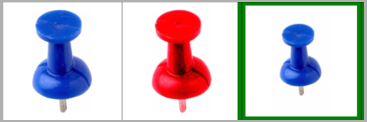
\includegraphics[width=\textwidth]{pics/size-sufficient.png}
\caption{Size sufficient.}
\label{fig:sizesufficient}
\end{subfigure}
\begin{subfigure}{.5\textwidth}
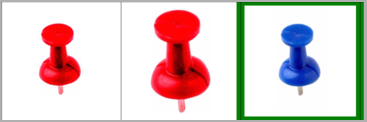
\includegraphics[width=\textwidth]{pics/color-sufficient.png}
\caption{Color sufficient.}
\label{fig:colorsufficient}
\end{subfigure}
\caption{Example contexts where (a) size only or (b) color only is sufficient for unique reference. A green border marks the intended referent.}
\label{fig:pin}
\end{figure}



\subsubsection{Asymmetry in redundant use of color and size adjectives}
\label{sec:asymmetry}

 In \figref{fig:sizesufficient}, singling out the object highlighted by the green border requires only mentioning its size (\emph{the small pin}). But it is now well-documented that speakers routinely include redundant color adjectives (\emph{the small blue pin}) which are not necessary for uniquely singling out the intended referent in these kinds of contexts \cite{Pechmann1989, Belke2002, gatt2011}. However, the same is not true for size: in contexts like \figref{fig:colorsufficient}, where color is sufficient for unique reference (\emph{the blue pin}), speakers overmodify much more rarely. Though there is quite a bit of variation in proportions of overmodification, this asymmetry in the propensity for overmodifying with color but not size has been documented repeatedly \cite{Pechmann1989, sedivy2003a,gatt2011, rubiofernandez2016,Westerbeek2015,Koolen2013}. 
 

Explanations for this asymmetry have varied. \citeA{Pechmann1989} was the first to take the asymmetry as evidence for speakers following an incremental strategy of object naming: speakers initially start to articulate an adjective denoting a feature that listeners can quickly and easily recognize (i.e., color) before they have fully inspected the display and extracted the sufficient dimension. However, this would predict that speakers routinely should produce expressions like \emph{the blue small pin}, which violate the preference for size adjectives to occur before color adjectives in English \cite{bloomfield1933, sproat1991}. While Pechmann did observe such violations in his dataset, most cases of overmodification did not constitute such violations, and he himself concluded that incrementality cannot (on its own) account for the asymmetry in speakers' propensity for overmodifying with color vs.~size. 


Another explanation for the asymmetry is that speakers try to produce modifiers that denote features that are reasonably easy for the listener to perceive, so that, even when a feature is not fully distinguishing in context, it at least serves to restrict the number of objects that could plausibly be considered the target. Indeed, there has been some support for the idea that overmodification can be beneficial to listeners by facilitating target identification \cite{Arts2011, rubiofernandez2016, Paraboni2007}. We return to this idea in \sectionref{sec:models} and the General Discussion.

%\jd{try to find a quote from someone who says it's all just a matter of cost?}

There have been various attempts to capture the color-size asymmetry in computational natural language generation models. The earliest contenders for models of definite referring expressions like the Full Brevity algorithm \cite{Dale1989} or the Greedy algorithm \cite{Dale1989} focused only on discriminatory value -- that is, an utterance's informativeness -- in generating referring expressions. This is equivalent to the very simple interpretation of Grice laid out above, and consequently these models demonstrated the same inability to capture the color-size asymmetry: they only produced the minimally specified expressions. Subsequently, the Incremental algorithm \cite{dale1995} incorporated a preference order on features, with color ranked higher than size. The order is traversed and each encountered feature included in the expression if it serves to exclude at least one further distractor. This results in the production of overinformative color but not size adjectives. However, the resulting asymmetry is much greater than that evident in human speakers, and is deterministic rather than exhibiting the probabilistic production patterns that human speakers exhibit. More recently, the PRO model \cite{GattEtAl2013} has sought to integrate the observation that speakers seem to have a preference for including color terms with the observation that a preference does not imply the deterministic inclusion of said color term. The model is specifically designed to capture the color-size asymmetry: in a first step, the uniquely distinguishing property (if there is one) is first selected deterministically. In a second step, an additional property is added probabilistically, depending on both a salience parameter associated with the additional property and a parameter capturing speakers' eagerness to overmodify. If both properties are uniquely distinguishing, a property is selected probabilistically depending on its associated salience parameter. The second step proceeds as before.

However, while the PRO model -- the most state-of-the-art computational model of human production of modified referring expressions -- can capture the color-size asymmetry in and of itself, it is neither flexible enough to be extended straightforwardly to other modifiers beyond color and size, nor can it straightforwardly be extended to capture the more subtle systematicity with which the preference to overmodify with color changes based on various features of context. 

\subsubsection{Scene variation}
\label{sec:scenevariation}

So far we have portrayed speakers' propensity to overmodify with color as a fixed quantity (though varying by experiment). However, this propensity is highly dependent on features of the distractor objects in the context. In particular, as the variation present in the scene increases, so does the probability of overmodifying  \cite{Davies2013, Koolen2013}. How exactly scene variation is quantified differs across experiments. One very clear demonstration of the scene variation effect was given by \citeA{Koolen2013}, who quantified scene variation as the number of feature dimensions along which objects in a scene vary. Over the course of three experiments, they compared a low-variation condition in which objects never differed in color with a high-variation condition in which objects differed in type, color, orientation, and size. They consistently found higher rates of overmodification with color in the high-variation (28-27\%) than in the low-variation (4-10\%) conditions. Similarly, \citeA{Davies2013} found that listeners judge overmodified referring expressions in low-variation scenes of four objects as less natural than in high-variation scenes of 4 potentially compositional `objects-on-objects' (e.g., a button on a sock). And finally, \citeA{gatt2017}, while not reporting differences in overmodification behavior, did find that when size and color are jointly disambiguating, speech onset times for non-redundant \emph{color-and-size} utterances increased as the number of distractors in the display increased.

The effect of scene variation on propensity to overmodify has typically been explained as the result of the demands imposed on visual search: in low-variation scenes, it is easier to discern the discriminating dimensions than in high-variation scenes, where it may be easier to simply start naming features of the target that are salient \cite{Koolen2013}. 


Above, we have considered three different ways of quantifying scene variation: the number of dimensions along which objects differ, whether objects are `simple' or `compositional', and the number of distractors present in a scene. A model of referring expression generation should ideally capture all of these types of variation in a unified way. 



\subsubsection{Feature typicality}
\label{sec:colortypicalityintro}

Modifier type and amount of scene variation are not the only factors determining overmodification. Overmodification with color has been shown to be systematically related to the typicality of the color for the object. Building on work by \citeA{sedivy2003a}, \citeA{Westerbeek2015} (and more recently, \citeA{rubiofernandez2016}) have shown that the more typical a color is for an object, the less likely it is to be mentioned when not necessary for unique reference. For example, speakers never refer to a yellow banana in the absence of other bananas as \emph{the yellow banana} (see \figref{fig:typical}), but they sometimes refer to a brown banana as \emph{the brown banana}, and they almost always refer to a blue banana as \emph{the blue banana} (see \figref{fig:atypical}). Similar typicality effects have been shown for other (non-color) properties. For example, \citeA{Mitchell2013} showed that speakers are more likely to include an atypical than a typical property (either shape or material) when referring to everyday objects like boxes when mentioning at least one property was necessary for unique reference. 

\begin{figure}
\begin{subfigure}{.5\textwidth}
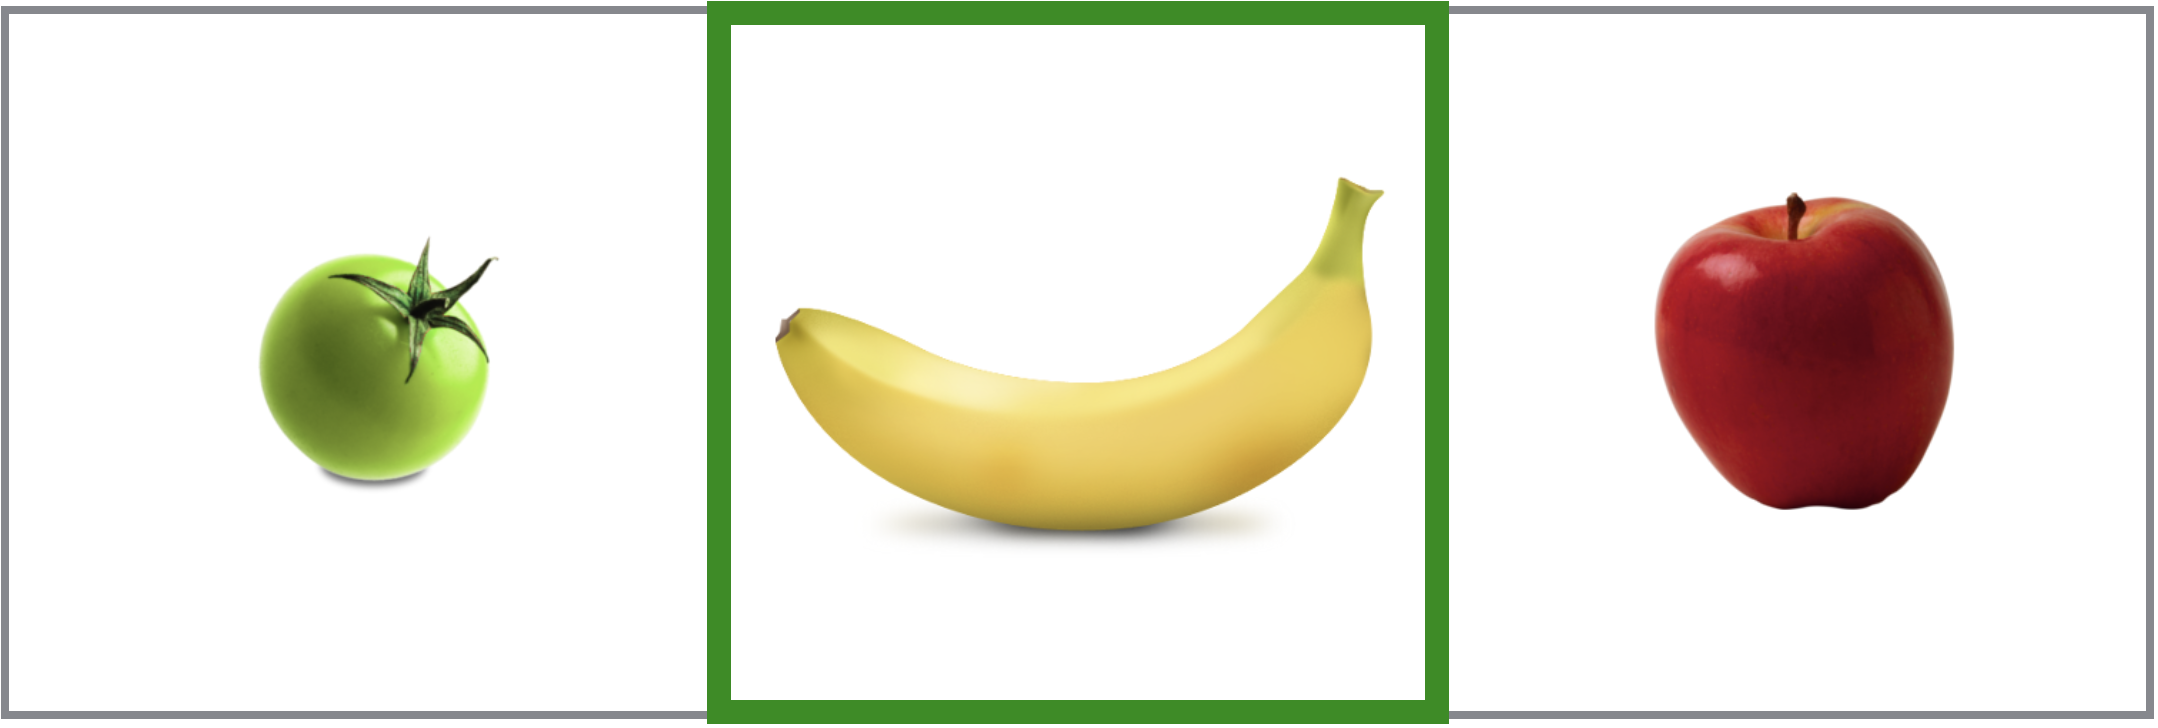
\includegraphics[width=\textwidth]{pics/banana-typical.png}
\caption{Typical color, type sufficient.}
\label{fig:typical}
\end{subfigure}
\begin{subfigure}{.5\textwidth}
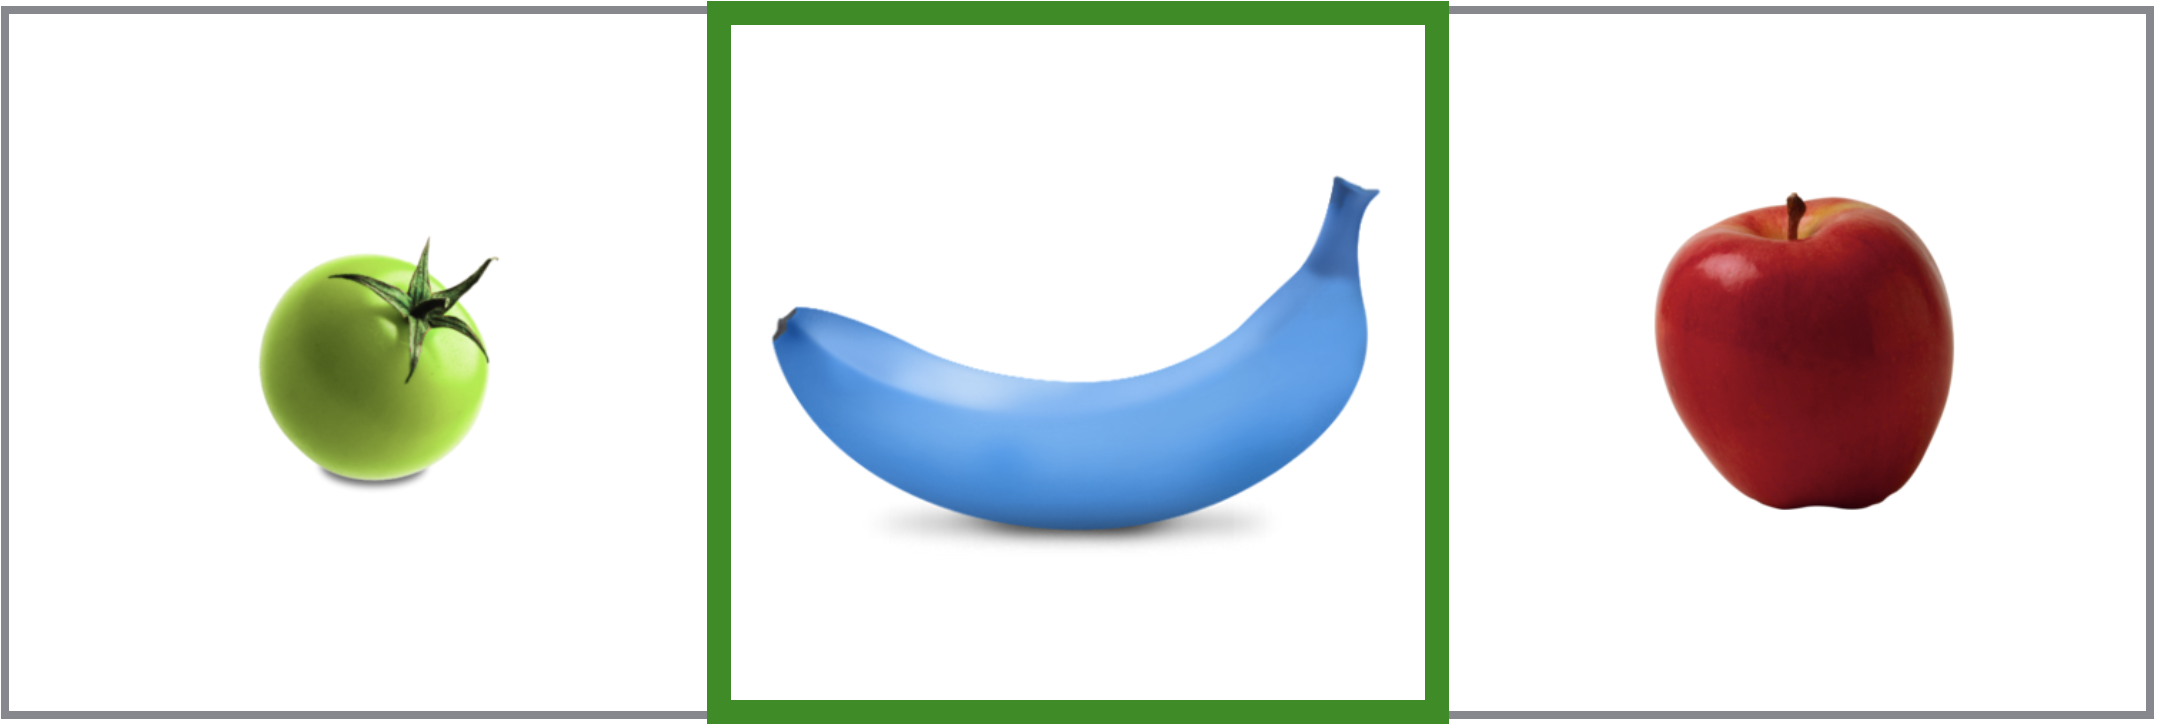
\includegraphics[width=\textwidth]{pics/banana-atypical.png}
\caption{Atypical color, type sufficient.}
\label{fig:atypical}
\end{subfigure}
\caption{Example contexts where type (\emph{banana}) is sufficient for unique reference and color is (a) typical or (b) atypical. A green border marks the intended referent.}
\label{fig:pin}
\end{figure}

Whether speakers are more likely to mention atypical properties over typical properties because they are more salient to \emph{them} or because they are trying to make reference resolution easier for the listener, for whom presumably these properties are also salient, is an open question \cite{Westerbeek2015}. Some support for the audience design account comes from a study by \citeA{Huettig2011}, who found that listeners, after hearing a noun with a diagnostic color (e.g., \emph{frog}), are more likely to fixate objects of that diagnostic color (green), indicating that typical object features are rapidly activated and aid visual search. Similarly, \citeA{Arts2011} showed that overspecified expressions result in faster referent identification.  Nevertheless, the benefit for listeners and the salience for speakers might simply be a happy coincidence and speakers might not, in fact, be designing their utterances for their addressees. We will remain agnostic about the underlying reason for typicality effects for the time being and will return to this issue in the General Discussion. 


\subsection{Nominal referring expressions}
\label{sec:nominalintro}

A problem related to the issue of how many additional features to include in a modified referring expression, but which has received much less attention in the language production literature, is that of deciding at which taxonomic level to refer to an object in a simple nominal expression. That is, even in the absence of adjectives, a referring expression can be more or less informative: \emph{the dalmatian} communicates more information about the object in question than \emph{the dog} (being a dalmatian entails being a dog), which in turn is globally more informative than \emph{the animal}. Thus, this choice can be considered analogous to the choice of adding more modifiers -- in both cases, the speaker has a choice of being more or less specific about the intended referent. However, the choice of reference level in simple nominal referring expressions is also interestingly different from that of adding modifiers in that there is no additional word-level cost associated with being more specific -- the choice is between different one-word utterances, not between utterances that differ in word length. 

Nevertheless, cognitive cost affects the choice of reference level: in particular, speakers prefer more frequent words over less frequent ones \cite{oldfield1965response}, and they prefer shorter ones over longer ones \cite{degen2013cost, rohde2012}. This may go part of the way towards explaining the well-documented effect from the concepts and categorization literature that speakers prefer to refer at the \emph{basic level} \cite{Rosch1976, Tanaka1991}. That is, in the absence of other constraints, even when a superordinate level term would be sufficient for establishing reference (as in \figref{fig:supersufficient}), speakers prefer to say \emph{the dog} rather than \emph{the animal}. 

Contextual informativeness is another factor that has been shown to affect speakers' nominal production choices \cite<e.g.,>{brennan1996}. For instance, in a context like \figref{fig:subnecessary}, speakers should use the subordinate level term \emph{dalmatian} to refer to the target marked with a green border, because a higher-level term (\emph{dog}, \emph{animal}) would be contextually underinformative.  However, there are nevertheless cases of contexts where either the superordinate \emph{animal} or the basic level \emph{dog} term would be sufficient for unique reference, as in  \figref{fig:supersufficient}, in which speakers nevertheless prefer to use the subordinate level term \emph{the dalmatian}. This is the case when the object is a particularly good instance of the subordinate level term or a particularly bad instance of the basic level term, compared to the other objects in the context. For example, penguins, which are rated as particularly atypical birds, are often referred to at the subordinate level \emph{penguin} rather than at the basic level \emph{bird}, despite the general preference for the basic level \cite{Jolicoeur1984}.


\begin{figure}
\begin{subfigure}{.5\textwidth}
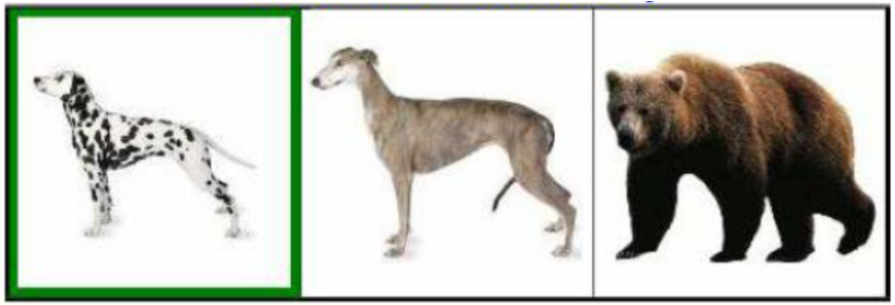
\includegraphics[width=\textwidth]{pics/dog-subnecessary}
\caption{Subordinate level term necessary.}
\label{fig:subnecessary}
\end{subfigure}
\begin{subfigure}{.5\textwidth}
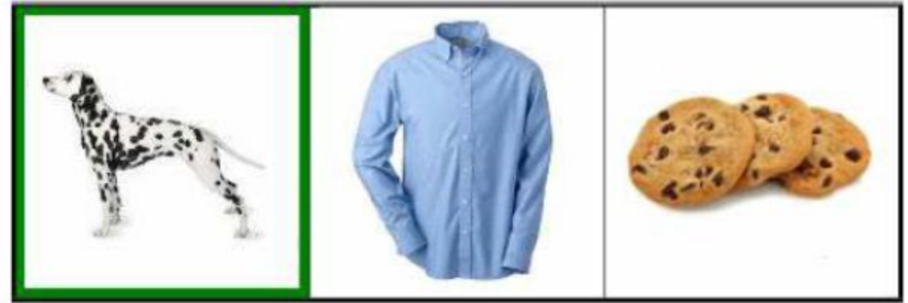
\includegraphics[width=\textwidth]{pics/dog-supersufficient}
\caption{Superordinate level term sufficient.}
\label{fig:supersufficient}
\end{subfigure}
\caption{Example contexts in which different levels of reference are necessary for establishing unique reference to the target marked with a green border. (a) subordinate (\emph{dalmatian}) necessary; (b) superordinate (\emph{animal}) sufficient, but basic  (\emph{dog}) or subordinate (\emph{dalmatian}) possible.}
\label{fig:dogexamples}
\end{figure}

\subsection{Summary}
\label{sec:introsummary}

In sum, the production of modified and simple nominal referring expressions is governed by many factors, including an utterance's informativeness, its cost relative to alternative utterances, and the typicality of an object or its features. 
Critically, these factors are all in play at once, potentially interacting in rich and complex ways.
In the next section, we provide an explicit computational account of these different factors and how they interact, with a focus on cases where speakers appear to be overinformative -- either by adding more modifiers or by referring at a more specific level than necessary for establishing unique reference. A summary of the effects we will focus on in the remainder of the paper is provided in \tableref{tab:effects}.

\begin{table}
\caption{List of effects a theory of referring expression production should account for and paper section(s) in which they are treated.}
\begin{tabular}{l l l } %p{5.5cm} }
\toprule
Section & Effect & Description \\ %& Reported by \\
\midrule
2 \& 3 & Color/size asymmetry & More redundant use of color than size \tablefootnote{Reported by many \cite<e.g.,>{Pechmann1989, Engelhardt2006, gatt2011, rubiofernandez2016}}\\ %&  \citeA{Pechmann1989, Engelhardt2006, gatt2011} \red{others}\\
%Number of distractors & More redundant use of color with increasing number of distractors & ?? \red{deutsch} \\
2 \& 3 & Scene variation & More redundant use of color with increasing scene variation \tablefootnote{Multiple replications reported \cite<e.g.,>{Davies2013, Koolen2013}}\\ %& \citeA{davies2009, Koolen2013}\\
\midrule
4 & Color typicality & More redundant use of color with decreasing color typicality \tablefootnote{Multiple replications reported \cite<e.g.>{sedivy2003a, Westerbeek2015, rubiofernandez2016}}\\ %& \citeA{sedivy2003aa, Westerbeek2015, rubiofernandez2016}\\
\midrule
5 & Basic level preference & Preference for basic level term when superordinate  sufficient \tablefootnote{Originally reported by \citeA{Rosch1976}, dozens of replications.}\\ %& \citeA{Rosch1976}\\
5 & Subordinate level use & Unnecessary use of subordinate level term  \tablefootnote{Reported by \citeA{Jolicoeur1984}}\\ %& \citeA{Jolicoeur1984}\\
\bottomrule
\end{tabular}
\label{tab:effects}
\end{table}


To date, there is no theory to account for all of these different phenomena; and no model has attempted to unify overinformativeness in the domain of modified and nominal referring expressions. We touched on some of the explanations that have been proposed for these phenomena. We also highlighted where computational models have been proposed for individual phenomena, and how they fall short. In the next section, we present the Rational Speech Act modeling framework, which we then use to capture these disparate phenomena in one model.


\section{Modeling speakers' choice of referring expression}
\label{sec:models}

Here we propose a computational model of referring expression production that accounts for the phenomena introduced above. The model is formulated within the Rational Speech Act (RSA) framework \cite{frank2012, goodman2016}.\footnote{All RSA models and Bayesian Data Analyses reported in this paper were implemented in the probabilistic programming language WebPPL \cite{GoodmanStuhlmuller14_DIPPL} and can be viewed at XXX.} It provides a principled explanation for the phenomena reviewed in the previous section and  holds promise for being generalizable to many further production phenomena related to overinformativeness, which we discuss in \sectionref{sec:gd}. We proceed by first presenting the general framework in \sectionref{sec:basicrsa}, and show why the most basic model, as formulated by \citeNP{frank2012}, does not produce the phenomena outlined above due to its strong focus on speakers maximizing the informativeness of expressions under a deterministic semantics. In \sectionref{sec:modifiedmodel} we introduce the crucial innovation: relaxing the assumption of a deterministic semantics. We show that the model can qualitatively account both for speakers' asymmetric propensity to overmodify with color rather than with size and (in \sectionref{sec:modelkoolen}) for speakers' propensity to overmodify more with increasing scene variation. 

%In \sectionref{sec:rsaevaluationbasicscene} we report an interactive  reference game experiment which functions as a quantitative test of the model. In \sectionref{sec:colortypicality} we explore how the model captures color typicality effects. In \sectionref{sec:nominal} we apply the model to the choice of simple nominal referring expressions. 

\subsection{Basic RSA}
\label{sec:basicrsa}

As has been pointed out by \citeA{GattEtAl2013}, the basic Rational Speech Act model as formulated by \citeA{frank2012} does not generate overinformative referring expressions for two reasons: first, it trivially cannot do so because it is limited to one-word utterances \cite<see also>{Baumann2014}. 
\ndg{why does everyone say this? the model was formulated for utterances, it was only applied to one word utterances...}\jd{because it's an easy strawman -- we can take this out, but we do need a hook}
But even when allowing two-word (or $n$-word) utterances, the speaker's utility function does not allow for producing redundant referring expressions as long as additional words contribute non-negative costs to the overall utterance cost. To see this, and as a basis for the innovation introduced in \sectionref{sec:modifiedmodel} it is useful to reiterate the basic form of the model.

The production component of RSA aims to soft-maximize the utility of utterances, where utility is defined in terms of the contextual informativeness of an utterance, given each utterance's literal semantics. Formally, this is treated as a pragmatic speaker $S_1$ reasoning about a literal listener $L_0$, who can be described by the following formula:

\begin{equation}
\label{eq:listener}
P_{L_0}(o | u) \propto \mathcal{L}(u,o).
%P_{L_0}(o | u) \propto \denote{u}(o).
%P_{L_0}(o | u) \propto \mathcal{U}(o|\{u \textrm{ is true of } o\}).
\end{equation}

%\begin{equation*}
%P_{L_0}(o | u) \propto \left\{
% \begin{array}{rl}
%  1 & \text{if } \denote{u}(o) = \text{true}\\
%   0 & \text{otherwise}
% \end{array} \right.
%\end{equation*}

The literal listener $L_0$ observes an utterance $u$ from the set of  utterances $U$, consisting of single adjectives denoting features available in the context of a set of objects  $O$, and returns a distribution over objects $o \in O$. Here, $\mathcal{L}(u,o)$ is the lexicon that encodes deterministic lexical meanings such that: 

\begin{equation}
\mathcal{L}(u,o) = \left\{
 \begin{array}{rl}
  1 & \text{if } u \text{ is true of } o\\
   0 & \text{otherwise}.
 \end{array} \right.
\end{equation}

%\begin{equation*}
%\denote{u}:O \rightarrow \{\text{true, false}\} 
%\end{equation*}
 Thus, $P_{L_0}(o | u)$ returns a uniform distribution over all contextually available $o$ in the extension of $u$. For example, in the size-sufficient context shown in \figref{fig:sizesufficient}, $U = \{\textrm{\emph{big}}, \textrm{\emph{small}}, \textrm{\emph{blue}}, \textrm{\emph{red}}\}$ and $O = \{o_{\textrm{big\_blue}}, o_{\textrm{big\_red}}, o_{\textrm{small\_blue}}\}$. Upon observing \emph{blue}, the literal listener therefore assigns equal probability to  $o_{\textrm{big\_blue}}$ and $o_{\textrm{small\_blue}}$. Values of $P_{L_0}(o | u)$ for each $u$ are shown on the left in \tableref{tab:detliteral}.

\begin{table}
%\centering
\caption{Row-wise literal listener distributions $P_{L_0}(o | u)$ for each utterance $u$ in the size-sufficient context depicted in \figref{fig:sizesufficient}, allowing only simple one-word utterances (left) or one- and two-word utterances (middle, right) under a deterministic semantics (left, middle) or under a continuous semantics (right) with  $x_{\text{size}} = .8$, $x_{\text{color}} = .99$. Bolded numbers indicate crucial comparisons between literal listener probabilities in correctly selecting the intended referent $o_{\text{small\_blue}}$ in response to observing the sufficient \emph{small} and the redundant \emph{small blue} utterances.}
%\begin{tabular}{l r r r}
%\toprule
%& $o_{\textrm{big\_blue}}$ & $o_{\textrm{big\_red}}$ & $o_{\textrm{small\_blue}}$ \\
%\midrule
%\emph{big} & .5 & .5 & 0\\
%\emph{small} & 0 & 0 & 1\\
%\emph{blue} & .5 & 0 & .5\\
%\emph{red} & 0 & 1 & 0\\
%\bottomrule
%\end{tabular}
\small
\begin{tabular}{l r r r r r r r r r}
\toprule
& \multicolumn{3}{c}{deterministic (simple)} & \multicolumn{3}{c}{deterministic (complex)} & \multicolumn{3}{c}{non-deterministic}\\
& $o_{\textrm{big\_blue}}$ & $o_{\textrm{big\_red}}$ & $o_{\textrm{small\_blue}}$ & $o_{\textrm{big\_blue}}$ & $o_{\textrm{big\_red}}$ & $o_{\textrm{small\_blue}}$
& $o_{\textrm{big\_blue}}$ & $o_{\textrm{big\_red}}$ & $o_{\textrm{small\_blue}}$ \\
\midrule
\emph{big} & .5 & .5 & 0 & .5 & .5 & 0 & .44 & .44 & .11 \\
\emph{small} & 0 & 0 & 1 & 0 & 0 & \textbf{1} & .17 & .17 & \textbf{.67} \\
\emph{blue} & .5 & 0 & .5 & .5 & 0 & .5 & .50 & .01 & .50 \\
\emph{red} & 0 & 1 & 0 & 0 & 1 & 0 & .01 & .99 & .01 \\
\emph{big blue} & NA & NA & NA & 1 & 0 & 0 & .79 & .01 & .20 \\
\emph{big red} & NA & NA & NA & 0 & 1 & 0 & .01 & .99 & .00 \\
\emph{small blue} & NA & NA & NA & 0 & 0 & \textbf{1} & .20 & .00 & \textbf{.80} \\
\bottomrule
\end{tabular}
\label{tab:detliteral}
\end{table}

The pragmatic speaker in turn produces an utterance with probability proportional to the utility of that utterance:

\begin{equation}
P_{S_1}(u | o) \propto e^{U(u,o)}
%P_{S_1}(u | o) \propto e^{\alpha \ln P_{L_0}(o | u) - \beta_c c(u)}
\end{equation}

The speaker's utility $U(u,o)$ is a function of both the utterance's \emph{informativeness}  with respect to the literal listener $P_{L_0}(o | u)$ and the utterance's \emph{cost} $c(u)$:

\begin{equation}
U(u,o) = \beta_{i} \ln P_{L_0}(o | u) - \beta_c c(u)
\end{equation}

Two free parameters, $\beta_i$ and $\beta_c$ enter the computation, weighting the respective contributions of informativeness and utterance cost, respectively.\footnote{\citeA{frank2012} fixed $\beta_i = 1$ and did not include cost in their formulation, because they assumed equal costs for all utterances. Subsequent work has demonstrated the importance of taking into account utterance cost in modeling  interpretation phenomena like cost-based quantity implicatures \cite{degenfrankejaeger2013} and M-implicature \cite{bergen2016}. We include it here because of the importance that cost has played in explanations of overinformative referring expressions, where it typically surfaces as the idea that speakers have different overall preferences for mentioning color vs.~size modifiers \cite{dale1995, Koolen2011, GattEtAl2013}. At this point we remain agnostic about the factors that contribute to an utterance's cost $c(u)$. In later sections we allow cost to be a function of properties (e.g. color \& size) mentioned in the utterance, or of an utterance's empirical length and corpus frequency; our policy for these cases is to introduce free cost parameters for each linear component of the cost function.}  In order to understand the effect of $\beta_i$, it is useful to explore its effect when utterances are cost-free. In this case, as $\beta_i$ approaches infinity, the speaker increasingly only chooses utterances that maximize informativeness; if $\beta_i$ is 0, informativeness is disregarded and the speaker chooses randomly from the set of all available utterances; if $\beta_i$ is 1, the speaker probability-matches, i.e., chooses utterances proportional to their informativeness \cite<equivalent to Luce's choice rule,>{luce1959}. Applied to the example in \tableref{tab:detliteral}, if the speaker wants to refer to $o_{\textrm{small\_blue}}$ they have two semantically possible utterances, \emph{small} and \emph{blue}, where \emph{small} is twice as informative as \emph{blue}. They produce \emph{small} with probability 1 when $\beta_i \rightarrow \infty$, probability 2/3 when $\beta_i = 1$ and probability 1/4 when $\beta_i = 0$.\footnote{Note that instead of a $\beta_i$ parameter weighting informativeness \emph{inside} the utility function, other recent formulations have used an $\alpha$ parameter modulating the entire utility function, i.e. $P_{S_1}(u |o)\propto \exp{\alpha U(u,o)}$. These parameterizations are equivalent. In the present work, where informativeness and cost both play important roles, we chose the `flattened' linear combination with independent weights for simplicity.}

%She will produce \emph{small} with the following probabilities as $\alpha$ varies: $P_{S_1}(\textrm{\emph{small}} | o_{\textrm{small\_blue}} ; \alpha = \infty) = 1$, $P_{S_1}(\textrm{\emph{small}} | o_{\textrm{small\_blue}} ; \alpha = 1) = \frac{2}{3}$, $P_{S_1}(\textrm{\emph{small}} | o_{\textrm{small\_blue}} ; \alpha = 0) = \frac{1}{4}$. 

Conversely, disregarding informativeness and focusing only on cost, any asymmetry in costs will be exaggerated with increasing $\beta_c$, such that the speaker will choose the least costly utterance with higher and higher probability as $\beta_c$ increases.

As noted above, this model does not generate redundant referring expressions for multiple reasons. One of these is trivial: $U$ only contains one-word utterances. We can ameliorate this easily by allowing complex two-word utterances. We assume an intersective semantics for complex utterances $u_{\textrm{complex}}$ that consist of a two adjective sequence $u_{\textrm{size}} \in \{\textrm{\emph{big}}, \textrm{\emph{small}}\}$ and $u_{\textrm{color}} \in \{\textrm{\emph{blue}}, \textrm{\emph{red}}\}$, such that the meaning of a complex two-word utterance is defined as
%\begin{equation} 
%\mathcal{L}(u_{\text{complex}},o) = \text{min}(\mathcal{L}(u_{\text{size}},o), \mathcal{L}(u_{\text{color}},o)).
%\end{equation} 

\begin{equation} 
\label{eq:prodcomp}
\mathcal{L}(u_{\text{complex}},o) = \mathcal{L}(u_{\text{size}},o) \times \mathcal{L}(u_{\text{color}},o).
\end{equation} 

The resulting renormalized literal listener distributions for our example size-sufficient context in \figref{fig:sizesufficient} are shown in the middle columns in \tableref{tab:detliteral}. 

Unfortunately, simply including complex utterances in the set of alternatives does not solve the problem. Let's turn again to the case where the speaker wants to communicate the small blue object. There are now two  utterances, \emph{small} and \emph{small blue}, which are both more informative than \emph{blue} and equally informative as each other, for referring to the small blue object. Because they are equally contextually informative, the only way for the complex utterance to be chosen with greater probability than the simple utterance is if it was the \emph{cheaper} one. While this would achieve the desired mathematical effect, the cognitive plausibility of complex utterances being cheaper than simple utterances is highly dubious. Even if it wasn't dubious: as  mentioned previously,  proportions of overinformative referring expressions are variable across experiments. The only way to achieve that variability under the basic model is to assume that the costs of utterances vary from task to task. This also seems to us an implausible assumption. Thus we must look elsewhere to account for overinformativeness. We propose that the place to look is the computation of informativeness itself. 

\subsection{RSA with continuous semantics -- emergent color-size asymmetry}
\label{sec:modifiedmodel}

Here we introduce the crucial innovation: rather than assuming a deterministic truth-conditional semantics that returns true (1) or false (0) for any combination of expression and object, we relax to a continuous semantics that returns real values in the interval $[0,1]$. 
Formally, the only change is in the values that the lexicon can return:
\begin{equation}
\mathcal{L}(u,o) \in [0, 1] \subset \mathbb{R}
\end{equation}
That is, rather than assuming that an object is unambiguously big (or not) or unambiguously blue (or not), this continuous semantics captures that objects count as big or blue to  varying degrees \cite<similar to approaches in fuzzy logic and prototype theory,>{zadeh1965fuzzy, Rosch1973}. 

An alternative, but equivalent, interpretation of the continuous semantics is as a form of noise or non-determinism in an otherwise truth-functional semantics. \ndg{showing this is kind of subtle... seems like we should put a brief argument here?}

The semantic value of utterance-object combinations can vary in complex ways, to be determined by lexical and compositional semantic rules.
To see the basic effect of switching to a continuous semantics, and to see how far we can get in capturing overinformativeness patterns with this change, let us explore a simple semantic theory in which all colors are treated the same, all sizes are as well, and the two compose via a product rule.
That is, when a size adjective would be `true' of an object under a deterministic semantics, we take $\mathcal{L}(u,o) = x_{\text{size}}$, a constant; when it is `false' of the object, $\mathcal{L}(u,o) = 1 - x_{\text{size}}$. 
Similarly for color adjectives. 
This results in two free model parameters, $x_{\text{size}}$ and $x_{\text{color}}$, that can take on different values, capturing that size and color adjectives may apply more or less well/reliably to objects.
Together with the product composition rule, Eq.~\ref{eq:prodcomp}, this fully specifies a relaxed semantic function for our reference domain.

Now consider the RSA literal listener, Eq.~\ref{eq:listener}, who uses these relaxed semantic values.
Given an utterance, the listener simply normalizes over potential referents. 
As an example, the resulting renormalized literal listener distributions for the size-sufficient example context in \figref{fig:sizesufficient} are shown for values $x_{\text{size}} = .8$ and $x_{\text{color}} = .99$  on the right in \tableref{tab:detliteral}. Recall that in this context, the speaker intends for the listener to select the small blue pin. To see which would be the best utterance to produce for this purpose, we can compare the literal listener probabilities in the $o_{\text{small\_blue}}$ column. The two best utterances under both the deterministic and the continuous semantics are bolded in the table: under the deterministic semantics, the two best utterances are \emph{small} and \emph{small blue}, with no difference in listener probability. In contrast, under the continuous semantics \emph{small} has a smaller literal listener probability (.67) of retrieving the intended referent than the redundant \emph{small blue}. Consequently, the pragmatic speaker will be more likely to produce \emph{small blue} than \emph{small}, though the precise probabilities depend on the cost and informativeness parameters $\beta_c$ and $\beta_i$. 

Crucially, the reverse is not the case when color is the distinguishing dimension. Imagine the speaker in the same context wanted to communicate the big red pin. The two best utterances for this purpose are \emph{red} (.99) and \emph{big red} (.99). In contrast to the results for the small blue pin, these utterances do not differ in their capacity to direct the literal listener to the intended referent. The reason for this is that we defined color to be almost noiseless, with the result that the literal listener distributions in response to utterances containing color terms are more similar to those obtained via a deterministic semantics than the distributions obtained in response to utterances containing size terms. The reader is encouraged to verify this by comparing the row-wise distributions under the  deterministic and continuous semantics in \tableref{tab:detliteral}.


To gain a wider understanding of the effects of assuming continuous meanings in contexts like that depicted in \figref{fig:sizesufficient}, we visualize the results of varying  $x_{\text{size}}$ and $x_{\text{color}}$ in \figref{fig:basicasymmetry}. To orient the reader to the graph: the deterministic semantics of utterances is approximated where the  semantic values of both size and color utterances are close to 1 (.999, top right-most point in graph).  In this case, the simple sufficient (\emph{small pin}) and complex redundant utterance (\emph{small blue pin}) are equally likely around .5, because they are both equally informative and utterances are assumed to have 0 cost. All other utterances are highly unlikely. The interesting question is under which circumstances, if any,  the standard color-size asymmetry emerges. This is the yellow/orange/red space in the `small blue' facet, characterized by values of $x_{\text{size}}$ that are lower than $x_{\text{color}}$, with high values for $x_{\text{color}}$. That is, redundant utterances are more likely than sufficient utterances when the redundant dimension (in this case color) is less noisy than the sufficient dimension (in this case size) and overall is close to noiseless. 

\begin{figure}
\centering
%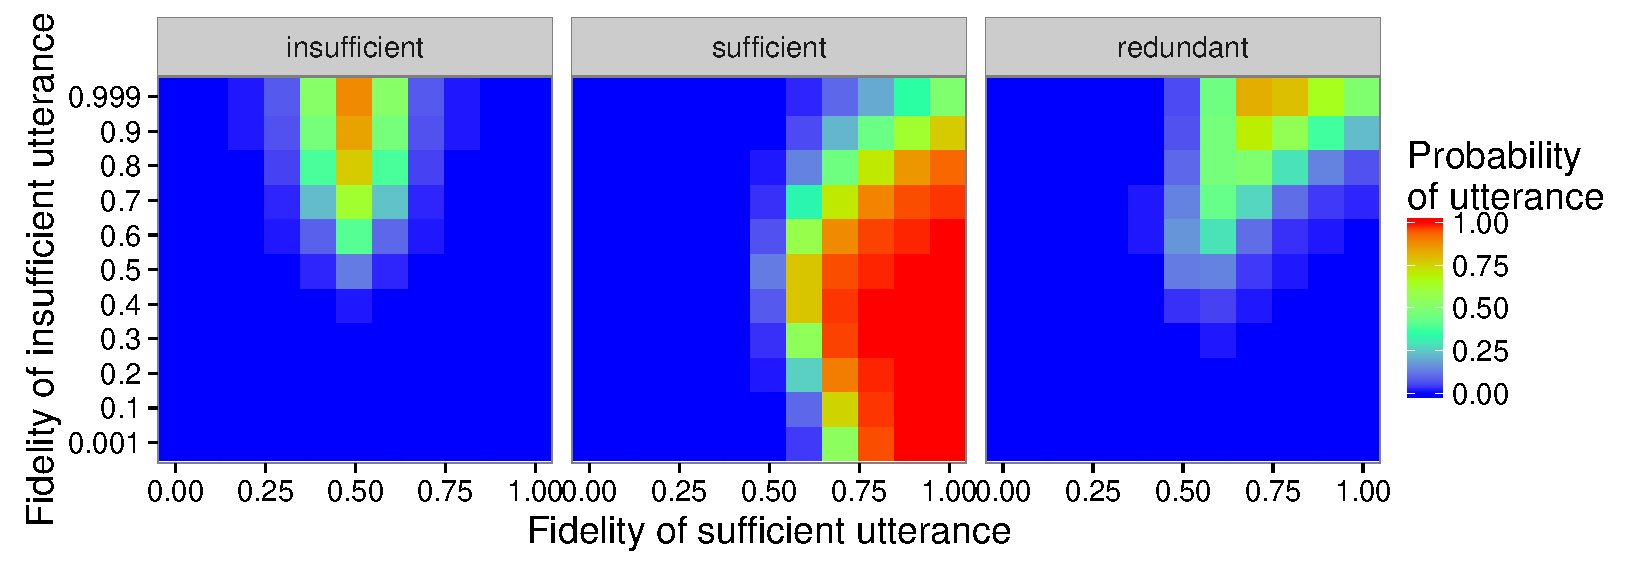
\includegraphics[width=\textwidth]{pics/modelexploration-fidelityeffect-unlogged-wide}
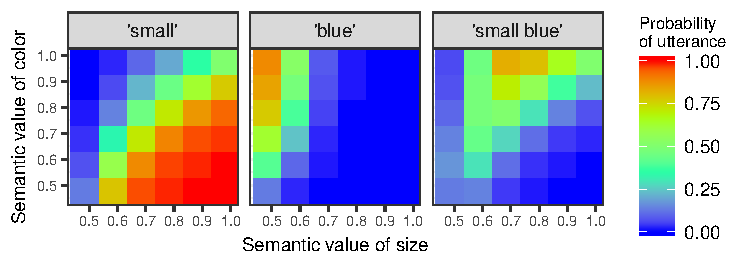
\includegraphics[width=.9\textwidth]{pics/modelexploration-fidelityeffect-paper}

\caption{Probability of producing sufficient \emph{small pin}, insufficient \emph{blue pin}, and redundant \emph{small blue pin} in contexts as depicted in \figref{fig:sizesufficient}, as a function of semantic value of color and size utterances (for $\beta_i = 30$ and $ \beta_c = 0$). For a visualization of model behavior under varying $\alpha$s, see \appref{app:modelexploration}.}
\label{fig:basicasymmetry}
\end{figure}

Thus, when size adjectives are noisier than color adjectives, the model produces overinformative referring expressions with color, but not with size -- precisely the pattern observed in the literature \cite{Pechmann1989, gatt2011}. Note also that no difference in adjective \emph{cost} is necessary for obtaining the overinformativeness asymmetry. However, assuming a greater cost for size than for color does further increase the observed asymmetry. We defer a discussion of costs to \sectionref{sec:exp1-scenevar}, where we infer the best parameter values for both the costs and the semantic values of size and color, given data from a reference game experiment.

We defer a complete discussion of the important potential psychological and linguistic interpretation of these continuous semantic values to the General Discussion in \sectionref{sec:gd}.
However, it is worth reflecting on why the size adjectives may be inherently noisier than color adjectives. Color adjectives are typically treated as  \emph{absolute adjectives} while size adjectives are inherently \emph{relative} \cite{kennedy2005}. That is, while both size and color adjectives are vague, size adjectives are arguably context-dependent in a way that color adjectives are not -- whether an object is big depends inherently on its comparison class; whether an object is red does not.\footnote{This is not entirely true, as has been repeatedly pointed out  \cite<e.g.,>{cohen1984models}: red hair has a very different color than red wine, which in turn has a different color from a red bell pepper. If presented out of context, only the last red is likely to be judged as red. %\ek{I found this: \cite{cohen1984models, halff1976context} 
For our purposes, it suffices that one can give a color judgment but not a size judgment for an object presented in isolation.} In addition, color as a property has been claimed to be inherently salient in a way that size is not \cite{Arts2011, GattEtAl2013}. Finally, we have shown in recent work that color adjectives are rated as less subjective than size adjectives \cite{scontras2017}. 
All of these suggest that size may be harder to pin down, and more likely to vary across people and contexts, than color.

To summarize, we have thus far shown that RSA with continuous adjective semantics can give rise to the well-documented color-size asymmetry in the production of overinformative referring expressions when color adjectives are closer to deterministic truth-functions than size adjectives. The crucial mechanism is this: when modifiers are relaxed, adding additional, stricter modifiers adds information. From this perspective, these redundant modifiers are not \emph{over}informative; they are rationally redundant, or sufficiently informative, given the needs of the listener. We spend the remainder of the paper demonstrating the far-reaching effects of assuming relaxed semantic values.

\subsection{RSA with continuous semantics -- scene variation}
\label{sec:modelkoolen}

As discussed in \sectionref{sec:intro}, increased scene variation has been shown to increase the probability of referring expressions that are overmodified with color. Here we simulate the experimental conditions reported by \citeA{Koolen2013} and explore continuous semantics RSA's predictions for these situations. \citeA{Koolen2013}  quantified scene variation as the number of feature dimensions along which pieces of furniture in a scene varied: type (e.g., chair, fan), size (big, small), and color (e.g., red, blue).\footnote{They also included orientation (left-facing, right-facing) as a dimension along which objects could vary in certain cases. We ignore this dimension here for the sake of simplicity.} Here, we  simulate the high and low variation conditions from their Experiments 1 and 2, reproduced in \figref{fig:koolencontexts}. 

In both conditions in both experiments, color was not necessary for establishing reference; that is, color mentions were always redundant. The two experiments differed in the dimension necessary for unique reference. In Exp.~1, only type was necessary (\emph{fan} and \emph{couch} in the low and high variation conditions in \figref{fig:koolencontexts}, respectively). In Exp.~2, size and type were necessary (\emph{big chair} and \emph{small chair} in \figref{fig:koolencontexts}, respectively). \citeA{Koolen2013} found lower rates of redundant color use in the low variation conditions (4\% and 9\%) than in the high variation conditions (24\% and 18\%).

We generated model predictions for precisely these four conditions. Note that by adding the type dimension as a distinguishing dimension, we must allow for an additional semantic value $x_{\text{type}}$, which encodes how noisy nouns are.

\begin{figure}
\begin{subfigure}{.5\textwidth}
%\includegraphics[width=.9\textwidth]{pics/Koolen2013-exp1}
%\includegraphics[width=.9\textwidth]{pics/Koolen2013-exp2}
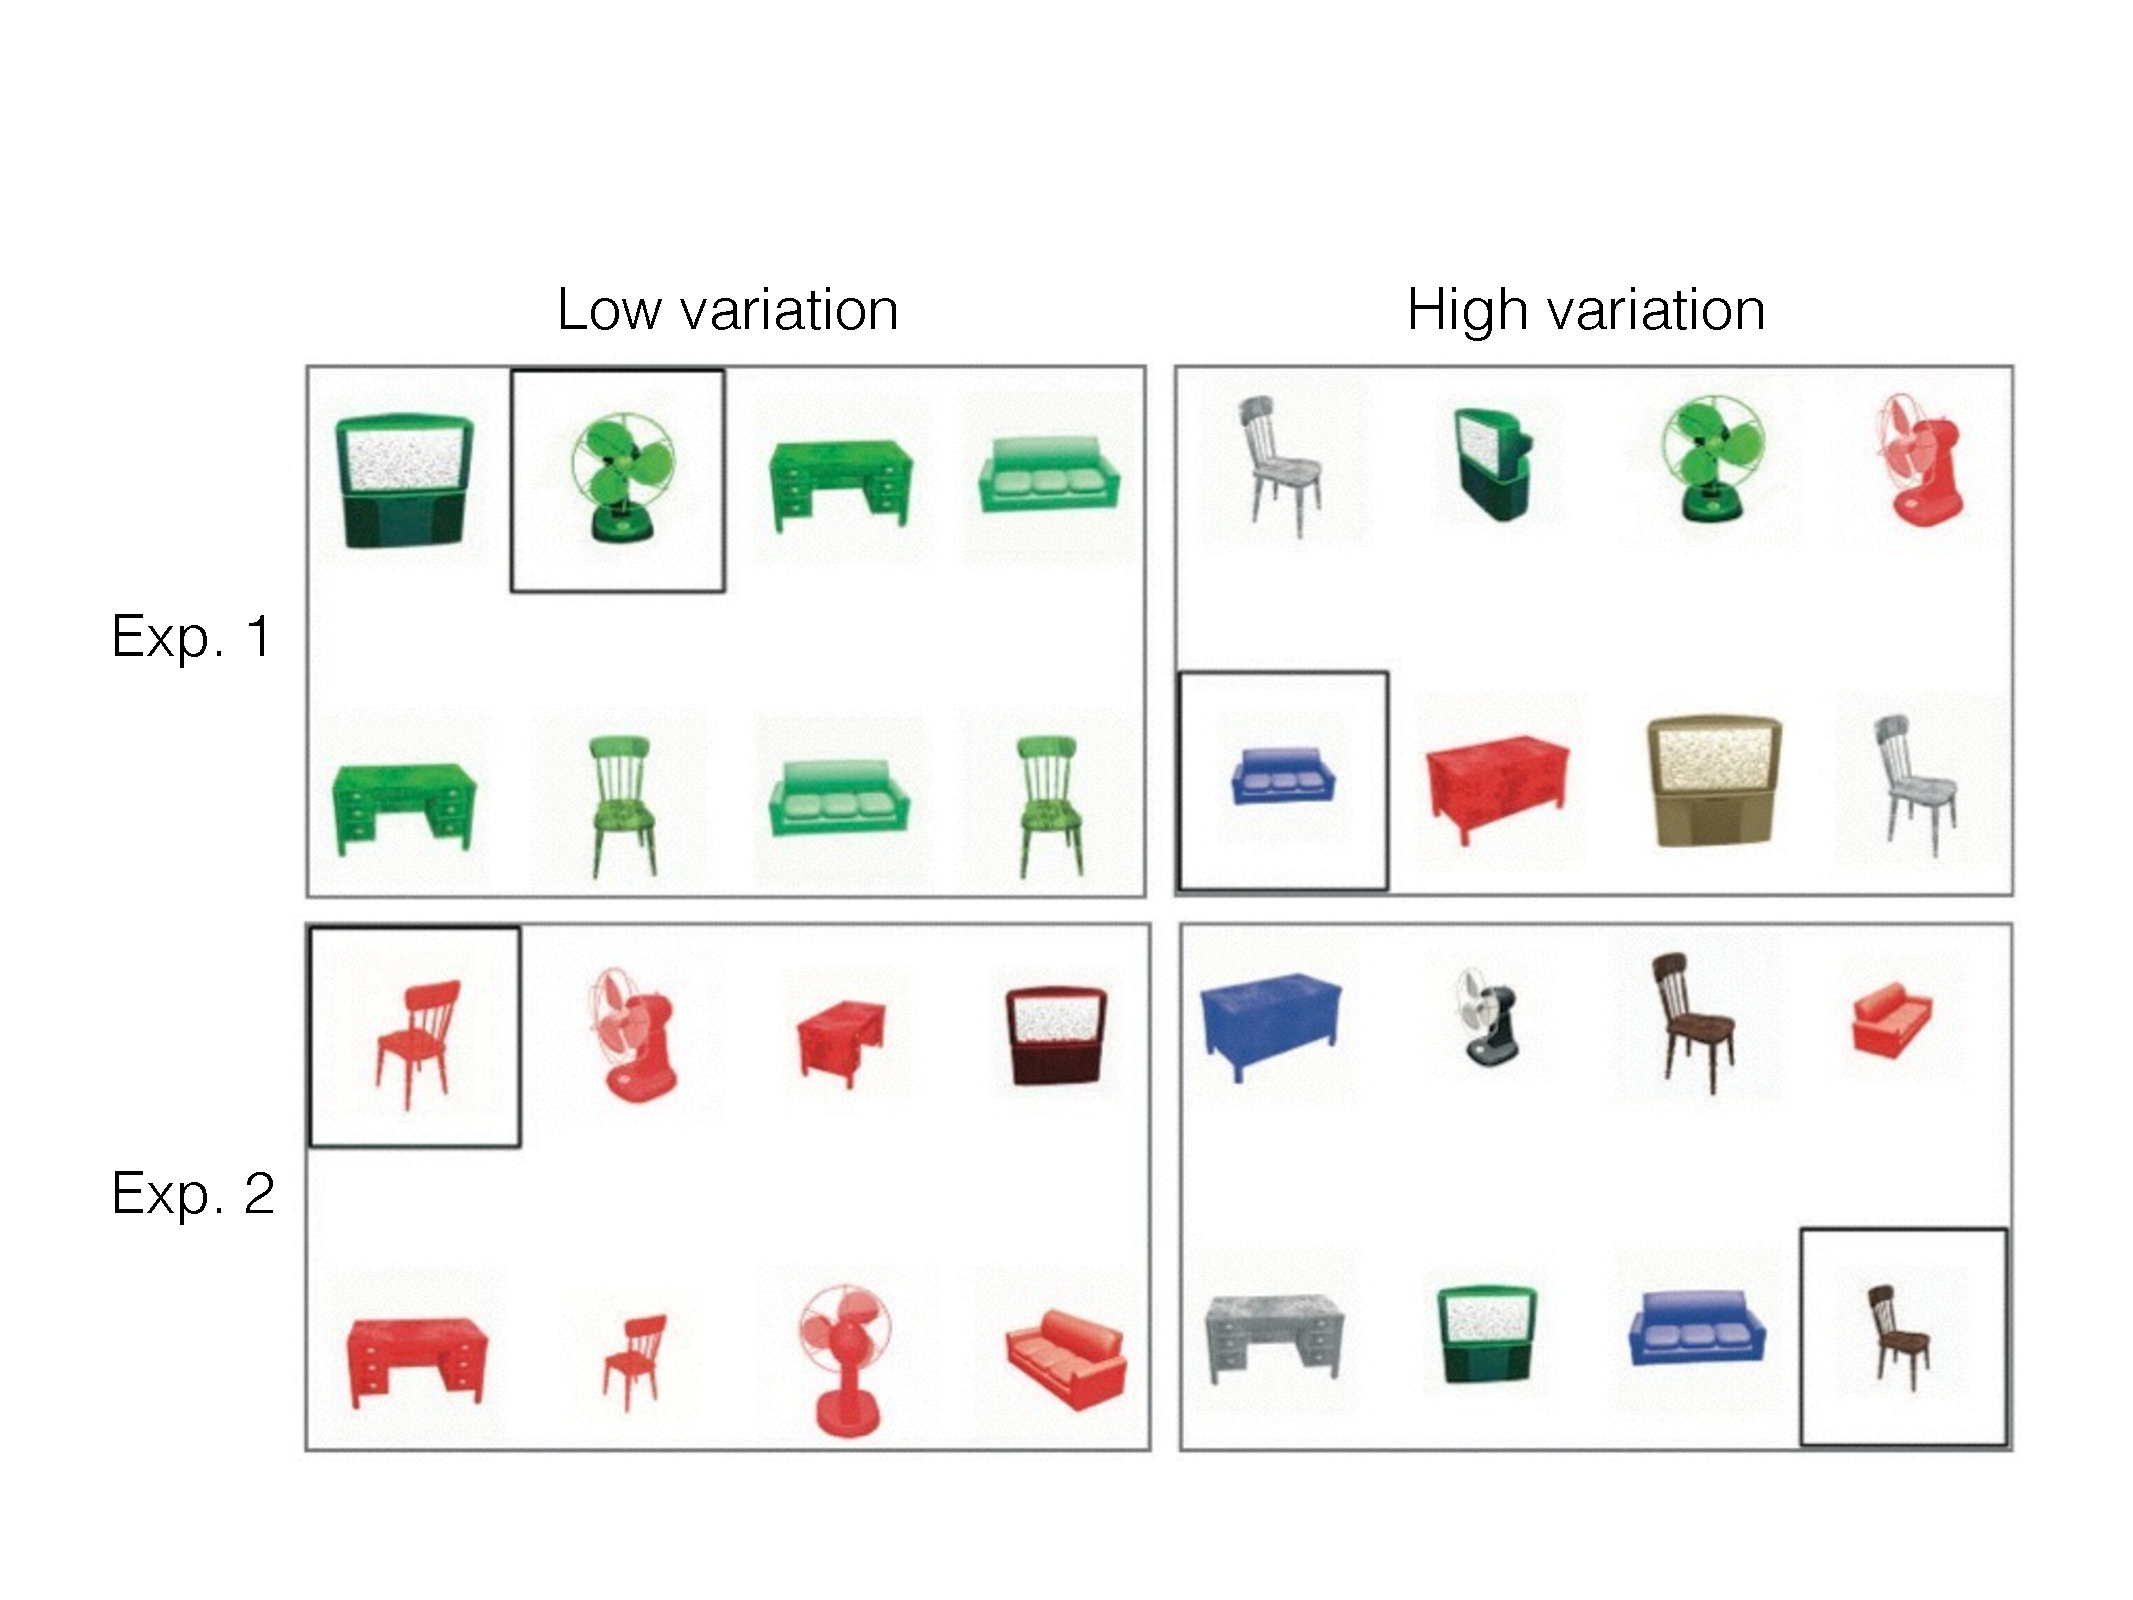
\includegraphics[width=\textwidth]{pics/koolen-conditions}
\caption{Contexts from Koolen et al.'s low variation (left column) and high variation (right column) conditions in Exp.~1 (top row) and Exp.~2 (bottom row).}
\label{fig:koolencontexts}
\end{subfigure}
\begin{subfigure}{.5\textwidth}
\centering
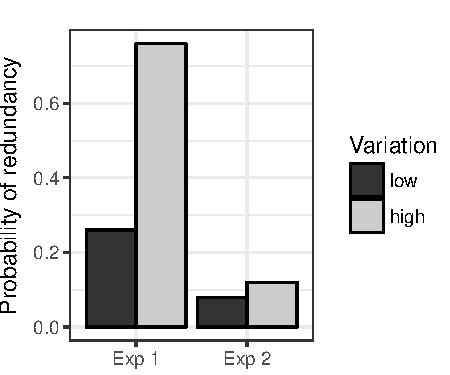
\includegraphics[width=.75\textwidth]{pics/koolen-effect}
\caption{Predicted probability of redundant color utterance in Koolen conditions for $\beta_i = 30$, $ \beta_c = c(u_{\textrm{size}}) = c(u_{\textrm{color}}) = 1$, $x_{\text{size}} = .8$, $x_{\text{color}} = .999$, $x_{\text{type}} = .9$.}
\label{fig:koolensimulationresults}
\end{subfigure}
\caption{Koolen et al.~contexts and RSA model predictions.}
\end{figure}

\citeA{Koolen2013} counted any mention of color as a redundant mention. In Exp.~1, this includes the simple redundant utterances like \emph{blue couch} as well as complex redundant utterances like \emph{small blue couch}. In Exp.~2, where size was necessary for unique reference, only the complex redundant utterance \emph{small brown chair} was truly redundant.  The results of simulating these conditions for $\beta_i = 30$, $ \beta_c = c(u_{\textrm{size}}) = c(u_{\textrm{color}}) = 1$, $x_{\text{size}} = .8$, $x_{\text{color}} = .999$, and $x_{\text{type}} = .9$ are shown in \figref{fig:koolensimulationresults}.%\footnote{See \appref{app:koolenexploration} for a visualization of model predictions under a fuller exploration of parameter combinations.}
\ndg{how were these values chosen? if they we fit to data, say so.}


\ndg{i don't believe we specified above that cost is the sum of word costs. i assume that's what we want here?}


For both experiments, the model retrieves the empirically observed qualitative effect of variation on the probability of redundant color mention: when variation is greater, redundant color mention is more likely. 
Indeed, the qualitative empirical scene variation effect is predicted by the model anytime the semantic values for size, type, and color are ordered as: $x_{\text{size}} \leq  x_{\text{type}} < x_{\text{color}}$. If $x_{\text{type}}$ is greater than $x_{\text{color}}$, the probability of redundantly mentioning color is close to zero and does not differ between variation conditions. This is because in those cases, color mention reduces, rather than adds, information about the target. 

\ndg{this stuff is pretty wishy washy...}
The absolute values predicted by the model ($\approx$ 8\% to $\approx$ 75\%) are different from the values observed by \citeA{Koolen2013}  ($\approx$ 4\% to $\approx$ 24\%).
Differences in exact values may stem from various sources. First, the best $\beta_i$ value to assume may differ from experiment to experiment. Second, semantic values may differ between experiments. Indeed, assuming a lower $x_{\text{color}}$  of .9 maintains the qualitative effects but lowers the highest probability of redundancy to .26 (which is much closer to the 24\% observed by Koolen et al). \ndg{so why didn't we use that value? how were the params set?}
Third, the values reported by \citeA{Koolen2013} were averaged over many different items -- here, we only reported model predictions for the example items they reported.


RSA with a continuous semantics thus captures the qualitative effects of color-size asymmetry and scene variation in production of redundant expressions. A quantitative test of the model will require larger data sets. 
In Sections 3, 4, and 5 we quantitatively evaluate continuous semantics RSA on datasets capturing the phenomena described in the Introduction (for a summary see \tableref{tab:effects}): modifier type and scene variation effects on modified referring expressions, typicality effects on color mention, and the choice of taxonomic level of reference in nominal choice, respectively.

\section{Modified referring expressions: size and color modifiers under different scene variation conditions}
\label{sec:rsaevaluationbasicscene}

Adequately assessing the explanatory value of RSA with non-deterministic truth functions requires evaluating how well it does at predicting the probability of various types of utterances occurring in large datasets of naturally produced referring expressions. To this end we proceed in two steps. First we report the results of a web-based interactive reference game in which we systematically manipulate scene variation (in a somewhat different way than \citeA{Koolen2013} did). We then perform Bayesian data analysis to generate model predictions, conditioning on the observed production data. This allows us to both a) assess  how likely the model is to generate the actually observed data -- i.e., to obtain a measure of model quality -- and b) infer the posterior probability of parameter values -- i.e., to understand whether the assumed asymmetries in the adjectives' semantic values and/or cost discussed in the previous section are warranted.


\subsection{Experiment 1: scene variation in modified referring expressions}
\label{sec:exp1-scenevar}

We saw in \sectionref{sec:modelkoolen} that continuous semantics RSA correctly predicts qualitative effects of scene variation on redundant adjective use. In particular, we saw that color is more likely to be used redundantly as the number of dimensions along which objects in a scene vary increases. However, we would like to a) go beyond a qualitative investigation of scene variation effects and also b) ask whether redundant size mention is also affected by scene variation. The notion of scene variation we employ is the proportion of distractor items that do not share the value of the insufficient feature with the target, that is, as the number of distractors $n_{\textrm{diff}}$ that differ in the value of the insufficient feature divided by the total number of distractors $n_{\textrm{total}}$:

\begin{equation*}
	\textrm{scene variation} = \frac{n_{\textrm{diff}}}{n_{\textrm{total}}}
\end{equation*}

To explain, let's turn again to \figref{fig:sizesufficient}. Here, the target item is the small blue pin and there are two distractor items: a big blue pin and a big red pin. Thus, for the purpose of establishing unique reference, size is the sufficient dimension and color the insufficient dimension. There is one distractor that differs from the target in color (the big red pin) and there are two distractors in total. That is, $\textrm{scenevar} = \frac{1}{2} = .5$. Scene variation is minimal when all distractors are of the same color as the target, in which case it is 0. Scene variation is maximal when all distractors except for one (in order for the dimension to remain insufficient for establishing reference) are of a different color than the target. That is, scene variation may take on values between 0 and $\frac{n_{\textrm{total} - 1}}{n_{\textrm{total}}}$, i.e, approaching but never reaching 1.\footnote{Some readers might find this unintuitive: shouldn't scene variation be maximal when there is an equal number of same and different colors? Or when the different colors are also all different from one another? As discussed in the Introduction, there are many ways of quantifying (different aspects of) scene variation. Here we explore just one such measure; it is an interesting question whether RSA accounts equally well for different ways of quantifying scene variation. Fortunately, it is very straightforward to implement such different measures by manipulating features of distractor items and exploring the model's behavior in these contexts.}

Using the same parameter values as in the previous two model explorations ($\beta_i = 30$, $ \beta_c = c(u_{\textrm{size}}) = c(u_{\textrm{color}}) = 1$, $x_{\text{size}} = .8$, $x_{\text{color}} = .999$), we generate model predictions for size-sufficient and color-sufficient contexts, varying scene variation by varying number of distractors (2, 3, or 4) and number of distractors that don't share the insufficient feature value. The resulting model predictions are shown in \figref{fig:numdistractors}: the probability of redundant adjective use increases with increasing scene variation when size is sufficient (and color redundant), but not when color is sufficient (and size redundant). This can be explained by noise distributions in the literal listener across contexts: in size-sufficient contexts, as the number of distractors of a different color than the target increases, using the relatively noiseless color term in addition to the more noisy size term reduces uncertainty about the target object more and more. However, the same is not true of the color-sufficient contexts: there is very little uncertainty about the target upon observing the minimal color utterance -- adding the size term only introduces more uncertainty about the target, regardless of the amount of scene variation. Note that this is highly dependent on the actual semantic value of color, with slightly lower semantic values for color, the model predicts small increases in redundant size use. This will be important for the interpretation of the empirical results. In general: increased scene variation is predicted to lead to a greater increase in redundant adjective use for less noisy adjectives.

\begin{figure}
\centering
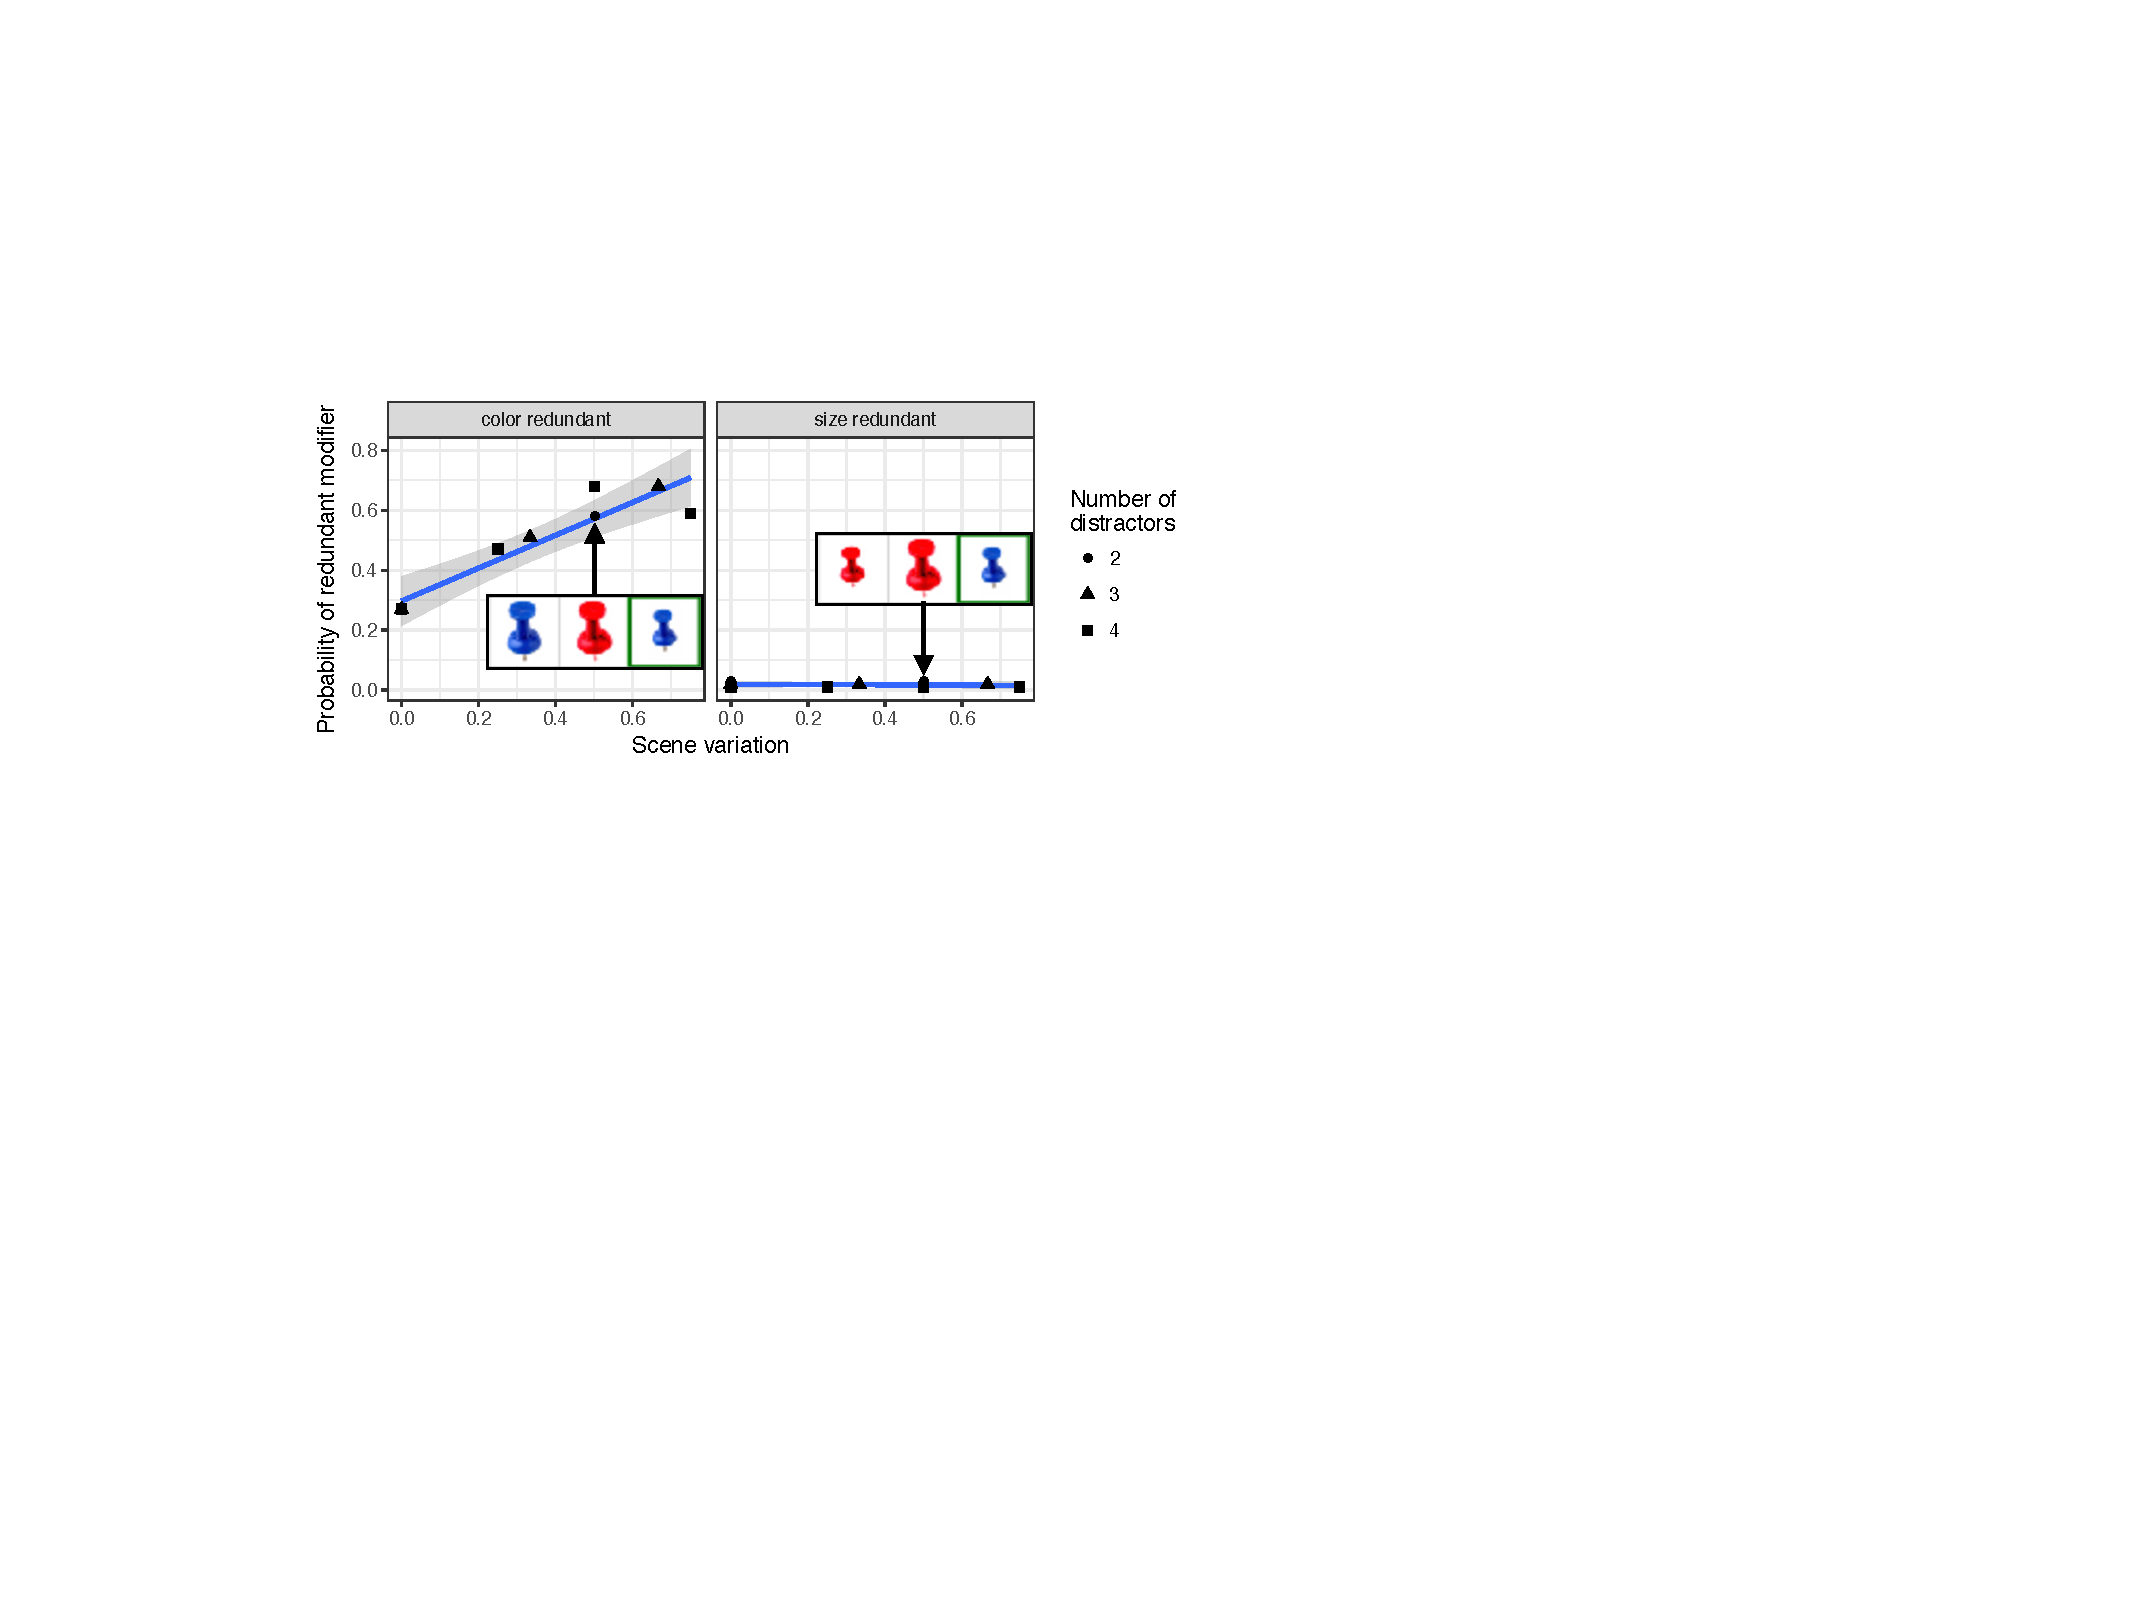
\includegraphics[width=.9\textwidth]{pics/scenevariation-annotation}
\caption{Probability of redundant utterance (\emph{small blue pin}) as a function of scene variation when size is sufficient (and color redundant, left) and when color is sufficient (and size redundant, right), for $\beta_i = 30$, $ \beta_c = c(u_{\textrm{size}}) = c(u_{\textrm{color}}) = 1$, $x_{\text{size}} = .8$, $x_{\text{color}} = .999$. Linear smoothers overlaid.}
\label{fig:numdistractors}
\end{figure}


To test continuous semantics RSA predictions, we conducted an interactive web-based written production study within a reference game setting. %\footnote{See \appref{app:replication}  for a validation of the general paradigm, in which we qualitatively replicate the findings of \citeA{gatt2011} with a different set of stimuli.} 
Speakers and listeners were shown arrays of objects that varied in color and size. Speakers were asked to produce a referring expression to allow the listener to identify a target object. We manipulated the number of distractor objects in the grid, as well as the variation in color and size among distractor objects.


\subsubsection{Method}

\paragraph{Participants}

We recruited 58 pairs of participants (116 participants total) over Amazon's Mechanical Turk who were each paid \$1.75 for their participation. Data from another 7 pairs who prematurely dropped out of the experiment and who could therefore not be compensated for their work, were also included. Here and in all other experiments reported in this paper, participants' IP address was limited to US addresses and only participants with a past work approval rate of at least 95\% were accepted. 

\paragraph{Procedure}

Participants were paired up through a real-time multi-player interface \cite{Hawkins15_RealTimeWebExperiments}. For each pair, one participant was assigned the speaker role and one the listener role. They  initially received written instructions that informed participants that one of them would be the Speaker and the other the Listener. They were further told that they would see some number of objects on each round and that the speaker's task is to communicate one of those objects, marked by a green border, to the listener. They were explicitly told that using locative modifiers (like \emph{left} or \emph{right}) would be useless because the order of objects on their partner's screen would be different than on their own screen. Before continuing to the experiment, participants were required to correctly answer a series of questions about the experimental procedure. These questions are listed in \appref{app:numdistractors}.

On each trial participants saw an array of objects. The array contained the same objects for both speaker and listener, but the order of objects was randomized and was typically different for speaker and listener. In the speaker's display, one of the objects -- henceforth the \emph{target} -- was highlighted with a green border. See \figref{fig:speakerlistenerperspective} for an example of the listener's and speaker's view on a particular trial.

\begin{figure}
\begin{subfigure}{.5\textwidth}
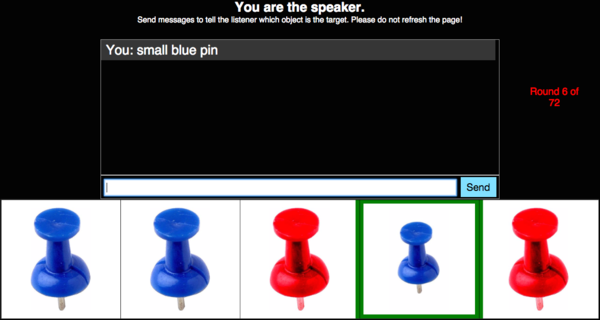
\includegraphics[width=\textwidth]{pics/speaker-perspective-small.png}
\caption{Speaker's perspective.}
\label{fig:speakerpersp}
\end{subfigure}
\begin{subfigure}{.5\textwidth}
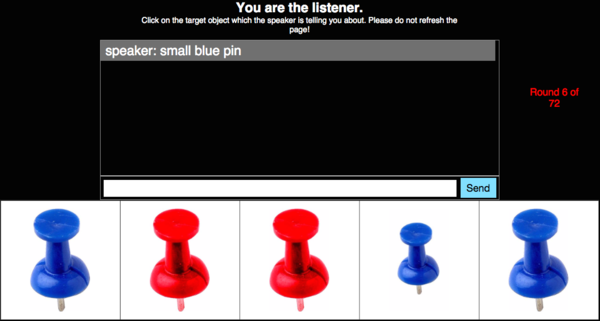
\includegraphics[width=\textwidth]{pics/listener-perspective-small.png}
\caption{Listener's perspective.}
\label{fig:listenerpersp}
\end{subfigure}
\caption{Example displays from the  (a) speaker's and the (b) listener's perspective on a \emph{size-sufficient 4-2} trial.}
\label{fig:speakerlistenerperspective}
\end{figure}

The speaker produced a referring expression to communicate the target to the listener by typing into an unrestricted chat window. After pressing Enter or clicking the `Send' button, the speaker's message was shown to the listener. The listener then clicked on the object they thought was the target, given the speaker's message.  Once the listener clicked on an object, a red border appeared around that object in both the listener and the speaker's display for 1 second before advancing to the next trial. That is, both participants received feedback about the speaker's intended referent and the listener's inference.

Both speakers and listeners could write in the chat window, allowing listeners to request clarification if necessary. Listeners could only click on an object and advance to the next trial once the speaker sent a message. 


\paragraph{Materials}

Participants proceeded through 72 trials. Of these, half were critical trials of interest and half were filler trials. On critical trials, we varied the feature that was sufficient to mention for uniquely establishing reference, the total number of objects in the array, and  the number of objects that shared the insufficient feature with the target. 

Objects varied in color and size. On 18 trials, color was sufficient for establishing reference. On the other 18 trials, size was sufficient. \figref{fig:speakerlistenerperspective} shows an example of a size-sufficient trial. We further varied the amount of variation in the scene by varying the number of distractor objects in each array (2, 3, or  4) and the number of distractors that did share the redundant feature value with the target. That is, when size was sufficient, we varied the number of distractors that shared the same color as the target. This number had to be at least one, since otherwise the redundant property would have been sufficient for uniquely establishing reference, i.e.~mentioning it would not have been redundant. Each total number of distractors was crossed with each possible number of distractors that shared the redundant property, leading to the following nine conditions: \emph{2-1, 2-2, 3-1, 3-2, 3-3, 4-1, 4-2, 4-3,} and \emph{4-4}, where the first number indicates the total number and the second number the shared number of distractors. Each condition occurred twice with each sufficient dimension. Objects never differed in type within one array (e.g., all objects are pins in \figref{fig:speakerlistenerperspective} but always differed in type across trials. Each object type could occur in two different sizes and two different colors. We deliberately chose photo-realistic objects of intuitively fairly typical colors. The 36 different object types and the colors they could occur with are listed in \appref{app:itemtypes}. 


Fillers were target trials from Exp.~2, a replication of \citeA{GrafEtAl2016}. Each filler item contained a three-object grid. None of the filler objects occurred on target trials. Objects stood in various taxonomic relations to each other and required neither size nor color mention for unique reference. See \sectionref{sec:nominal} for a description of these materials.

\subsubsection{Data pre-processing and exclusion}

We collected data from 2177 critical trials. Because we did not restrict participants' utterances in any way, they produced many different kinds of referring expressions. Testing the model's predictions required, for each trial, classifying the produced utterance as an instance of a \emph{color}-only mention, a \emph{size}-only mention, or a \emph{color-and-size} mention (or excluding the trial if no classification was possible). To this end we conducted the following semi-automatic data pre-processing. 

An R script first automatically checked whether the speaker's utterance contained a precoded color (i.e. \emph{black, blue, brown, gold, green, orange, pink, purple, red, silver, violet, white, yellow}) or size (i.e. \emph{big, bigger, biggest, huge, large, larger, largest, little, small, smaller, smallest, tiny}) term. In this way, 95.7 \% of cases were classified as mentioning size and/or color. However, this did not capture that sometimes, participants produced meaning-equivalent modifications of color/size terms for instance by adding suffixes (e.g., \emph{bluish}), using abbreviations (e.g., \emph{lg} for \emph{large} or \emph{purp} for \emph{purple}), or using non-precoded color labels (e.g., \emph{lime} or \emph{lavender}). Expressions containing a typo (e.g., \emph{pruple} instead of \emph{purple}) could also not be classified automatically. In the next step, one of the authors (CG) therefore manually checked the automatic coding to include these kinds of modifications in the analysis. This covered another 1.9\% of trials. Most of the time, participants converged on a convention of producing only the target's size and/or color, e.g., \emph{purple} or \emph{big blue}, but not an article (e.g., \emph{the}) or the noun corresponding to the object's type  (e.g., \emph{comb}). Articles were omitted in 88.6 \% of cases and nouns were omitted in 71.6 \% of cases. We did not analyze this any further.

There were 50 cases (2.3\%) in which the speaker made reference to the distinguishing dimension in an abstract way, e.g.~\emph{different color}, \emph{unique one}, \emph{ripest}, \emph{very girly}, or \emph{guitar closest to viewer}. While interesting as utterance choices,\footnote{Certain participants seemed to have deliberately used this as a strategy even though simply mentioning the distinguishing property would have been shorter in most cases. In all, only 12 participants produced these kinds of utterances: one 18 times, one 8 times, one 6 times, two 3 times, one 2 times, and the remaining six only once each.} these cases were excluded from the analysis. There were 3 cases that were nonsensical, e.g. \emph{bigger off a shade}, which were also excluded. In 6 cases only the insufficient dimension was mentioned -- these were excluded from the analysis reported in the next section, where we are only interested in minimal or redundant utterances, not underinformative ones, but were included in the Bayesian data analysis reported in \sectionref{sec:modifiermodeleval}. Finally, we excluded six trials where the speaker did not produce any utterances, and 33 trials on which the listener selected the wrong referent, leading to the elimination of 1.5\% of trials. After the exclusion, 2076 cases classified as one of \emph{color}, \emph{size}, or \emph{color-and-size} entered the analysis. After the exclusion, 2076 cases classified as one of \emph{color}, \emph{size}, or \emph{color-and-size} entered the analysis.

\subsubsection{Results}
\label{sec:modelempiricalresults}
% The analysis R script is in writing/2016/theory/rscripts/analysis_modifiers.R

Proportions of redundant \emph{color-and-size} and minimal \emph{color} or \emph{size} utterances are shown in \figref{fig:exp1results} alongside model predictions (to be explained further in \sectionref{sec:modifiermodeleval}). There are three main questions of interest: first, do we replicate the color/size asymmetry in probability of redundant adjective use? Second, do we replicate the previously established effect of increased redundant color use with increasing scene variation? Third, is there an effect of scene variation on redundant size use and if so, is it smaller compared to that on color use, as is predicted under asymmetric semantic values for color and size adjectives?

\begin{figure}
\centering
%\includegraphics[width=\textwidth]{../../../models/1a_bda_basic/results_bda/graphs/scenevariation-fixed-reducedconditions}
%old location: \includegraphics[width=.7\textwidth]{../../../models/old/1a_bda_basic/results_bda/graphs/scenevariation-fixed-reducedconditions-unlogged}
%\includegraphics[width=\textwidth]{pics/scenevariation-fixed-reducedconditions-unlogged}
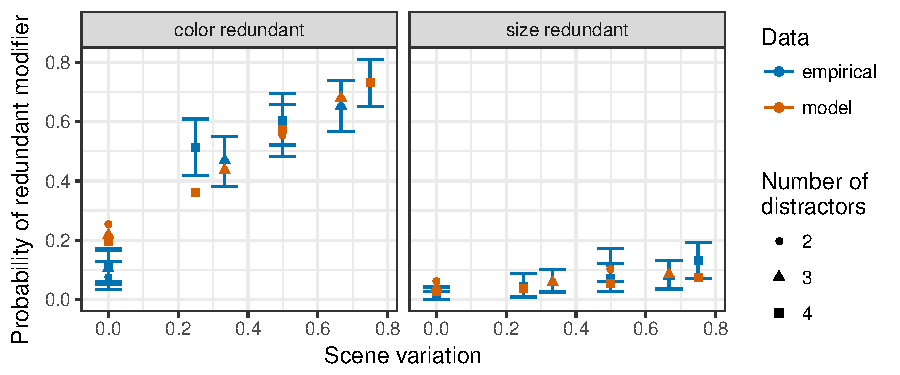
\includegraphics[width=.9\textwidth]{pics/exp1-empirical-predictives}
\caption{Empirical utterance proportions  (red)  alongside point-wise maximum a posteriori (MAP) estimates of the RSA model's posterior predictives for utterance probability (blue) as a function of scene variation. Rows indicate the sufficient dimension, columns the produced utterance. Here and in all following plots, error bars indicate 95\% bootstrapped confidence intervals.}
\label{fig:exp1results}
\end{figure}

We addressed all of these questions in one fell swoop by conducting a mixed effects logistic regression analysis predicting redundant over minimal adjective use from fixed effects of sufficient property (color vs.~size), scene variation (proportion of distractors that does not share the insufficient property value with the target), and the interaction between the two.\footnote{All mixed effects analyses reported in this paper were conducted with the \verb+lme4+ package \cite{lme4} in R \cite{R}.} The model included the maximal random effects structure that allowed the model to converge: by-speaker and by-item random intercepts.\footnote{In order to address convergence issues with \verb+lmer+ when specifying the full random effects structure -- i.e., by-speaker and by-item random intercepts and slopes for all fixed effects and their interactions -- we ran a Bayesian binomial mixed effects model with weakly informative priors using the \verb+brms+ package \cite{brms} that included the same fixed effects structure as the lmer model and the full random effects structure. The results were qualitatively identical, yielding  evidence for main effects of redundant feature (posterior mean $\beta$ = 5.91, $95\%$ CI = $[$4.15,8.10$]$, $p(\beta > 0)$ = .98), scene variation (posterior mean $\beta$ = 6.18, $95\%$ CI = $[$4.30,8.24$]$, $p(\beta > 0)$ = 1), and their interaction (posterior mean $\beta$ = 3.31, $95\%$ CI = $[$-0.54,7.23$]$, $p(\beta > 0)$ = .96).}

We observed a main effect of sufficient property, such that speakers were more likely to redundantly use color than size adjectives ($\beta = 3.54$, $SE = .22$, $p < .0001$), replicating the much-documented color-size asymmetry. We further observed a main effect of scene variation, such that redundant adjective use increased with increasing scene variation ($\beta = 4.62$, $SE = .38$, $p < .0001$). Finally, we also observed a significant interaction between sufficient property and scene variation ($\beta = 2.26$, $SE = .74$, $p < .003$). Simple effects analysis revealed that the interaction was driven by the scene variation effect being smaller in the \emph{color-sufficient} condition ($\beta = 3.49$, $SE = .65$, $p < .0001$) than in the \emph{size-sufficient} condition ($\beta = 5.75$, $SE = .38$, $p < .0001$), as predicted if size modifiers are noisier than color modifiers.


\subsection{Model evaluation}
\label{sec:modifiermodeleval}

% Extra info: 10000 samples, burn 3000, uniform drift, acceptance rate .4

In order to evaluate RSA with non-deterministic truth functions, we asked how well it captures the empirical data. To this end we conducted a Bayesian data analysis.  This allowed us to  simultaneously generate model predictions and infer likely parameter values, by conditioning on the observed production data (coded into \emph{size}, \emph{color}, and \emph{size-and-color} utterances as described above) and integrating over the five free parameters. To allow for differential costs for size and color, we introduce separate cost weights ($\beta_{c(\textrm{size})}, \beta_{c(\textrm{color})}$) applying to size and color mentions, respectively, in addition to semantic values for color and size ($x_{\textrm{color}}$, $x_{\textrm{size}}$) and an informativeness parameter $\beta_i$. We assumed uniform priors for each parameter: $x_{\textrm{color}}, x_{\textrm{size}} \sim \mathcal{U}(0,1)$,  $\beta_{c(\textrm{size})}, \beta_{c(\textrm{color})} \sim \mathcal{U}(0,40)$, $\beta_i  \sim \mathcal{U}(0,40)$.
Inference for the cognitive model was exact. We used Markov Chain Monte Carlo (MCMC) with a burn-in of 10000 and lag of 10 to draw 2000 samples from the joint posteriors on the five free parameters.

% JD: throwing out the scatterplot because it doesn't add anything
%\begin{figure}
%\centering
%%old location: \includegraphics[width=.7\textwidth]{../../../models/old/1a_bda_basic/results_bda/graphs/predictives-collapsed-fixed-reducedconditions-unlogged}
%\includegraphics[width=.7\textwidth]{pics/predictives-collapsed-fixed-reducedconditions-unlogged}
%\caption{Scatterplot of point-wise maximum a posteriori (MAP) estimates of the RSA model's posterior predictives against empirical proportions ($r=$.85). \jd{update this plot once bda run}}
%\label{fig:modelexp1scatter}
%\end{figure}

Point-wise maximum a posteriori (MAP) estimates of the model's posterior predictives for each combination of utterance, sufficient dimension, number of distractors, and number of different distractors (collapsing across different items) are compared to empirical data in \figref{fig:exp1results}. At this level, the model achieves a correlation of $r = .99$. Looking at results additionally on the by-item level yields a correlation of $r = .85$. The model thus does a very good job of capturing the quantitative patterns in the data. %The only clear flaw is that the model predicts greater redundant adjective use than empirically observed when there is no scene variation at all. \jd{Though this is a pretty minor thing. Noah, can you add a sentence on why, given that you've thought about this for the negation case as well? Or should we just leave it out?}.



Posteriors over parameters are shown in \figref{fig:modifierparamposteriors}. Crucially, the semantic value of color is inferred to be higher than that of size -- there is no overlap between the 95\% highest density intervals (HDIs) for the two parameters. That is, size modifiers are inferred to be noisier than color modifiers. The  high inferred $\beta_i$ (MAP $\beta_i$ = 31.4, HDI = [30.7,34.5]) suggests that this difference in semantic value contributes substantially to the observed color-size asymmetries in redundant adjective use and that speakers are maximizing quite strongly. As for cost, there is a lot of overlap in the inferred weights of size and color modifiers, which are both skewed very close to zero, suggesting that a cost difference (or indeed any cost at all) is neither necessary  to obtain the color-size asymmetry and the scene variation effects, nor justified by the data. Recall further that we already showed in \sectionref{sec:modifiedmodel}  that the color-size asymmetry in redundant adjective use requires an asymmetry in semantic value and cannot be reduced to cost differences. An asymmetry in cost only serves to further enhance the asymmetry brought about by the  asymmetry in semantic value, but cannot carry the redundant use asymmetry on its own.


\begin{figure}
\centering
%\includegraphics[width=\textwidth]{../../../models/1a_bda_basic/results_bda/graphs/parameterposteriors-fixed-reducedconditions}
% old location \includegraphics[width=\textwidth]{../../../models/old/1a_bda_basic/results_bda/graphs/parameterposteriors-fixed-reducedconditions-unlogged}
%\includegraphics[width=\textwidth]{pics/parameterposteriors-fixed-reducedconditions-unlogged}
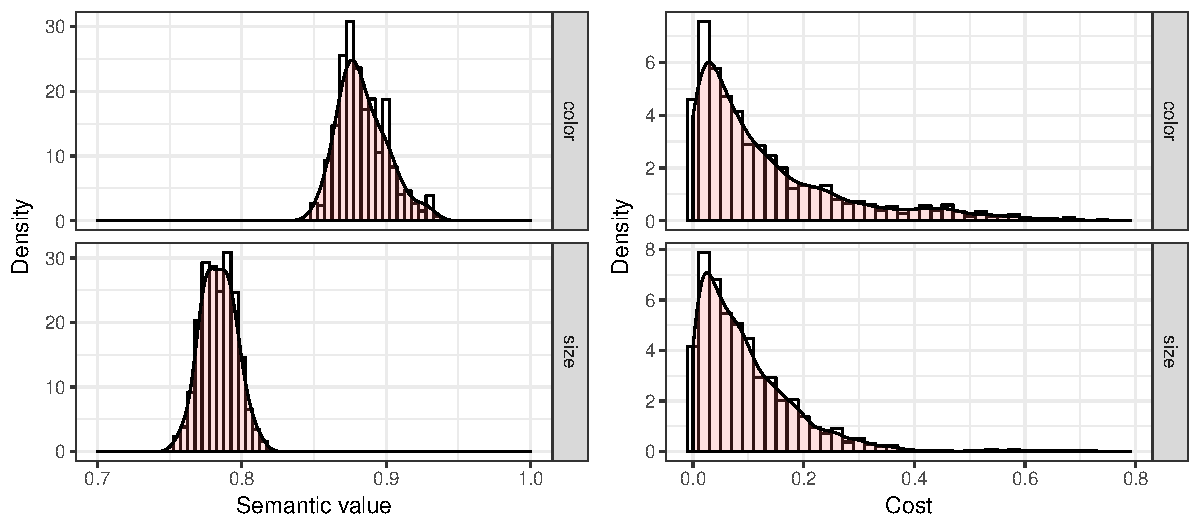
\includegraphics[width=\textwidth]{pics/exp1-paramposteriors}
\caption{Posterior model parameter distributions for semantic value (left column) and cost (right column), separately for color (top row) and size (bottom row). Maximum a posteriori (MAP)  $x_{\textrm{size}}$ = 0.79, 95\% highest density interval (HDI) = [0.76,0.80]; MAP $x_{\textrm{color}}$ = 0.88, HDI = [0.85,0.92]; MAP $\beta_{c(\textrm{size})}$ = .02, HDI = [0, 0.26]; MAP $\beta_{c(\textrm{color})}$ = 0.03, HDI = [0,0.45].}
\label{fig:modifierparamposteriors}
\end{figure}

\subsection{Discussion}
\label{sec:modifierdiscussion}

In this section, we reported the results of a dataset of freely collected referring expressions that replicated the well-documented color-size asymmetry in redundant adjective, the effect of scene variation on redundant color use, and showed a novel effect of scene variation on redundant size use. We also showed that continuous semantics RSA provides an excellent fit to these data. In particular, the crucial element in obtaining the color-size asymmetry in overmodification is that size adjectives be noisier than  color adjectives, captured in RSA via a lower semantic value for size compared to color. The effect is that color adjectives are more informative than size adjectives when controlling for the number of distractors each would rule out under a deterministic semantics. Asymmetries in the cost of the adjectives  only serve to further enhance the modification asymmetry resulting from the asymmetry in semantic value. In addition, we showed that asymmetric effects of scene variation on overmodification straightforwardly fall out of continuous semantics RSA: scene variation leads to a greater increase in overmodification with less noisy than with more noisy modifiers because the less noisy modifiers (colors) on average provide more information about the target.

Some readers may find themselves wondering about the status of these semantic values: are we claiming that color modifiers have inherently higher semantic values than size modifiers? Is the difference constant? What if the color modifier is a less well known one like \emph{mauve}? The way we have set the model up thus far, there would indeed be no difference in semantic value between \emph{red} and \emph{mauve}. Moreover, the model is not equipped to handle potential object-level idiosyncracies such as the typicality effects discussed in \sectionref{sec:colortypicalityintro}. We defer a fuller discussion of the status of the semantic value term to the General Discussion and turn first to continuous semantics RSA's potential for capturing these typicality effects.

\jd{will have to discuss here already and then just summarize in GD}

\section{Modified referring expressions: color typicality}
\label{sec:colortypicality}


In \sectionref{sec:rsaevaluationbasicscene} we showed that continuous semantics RSA successfully captures both the basic asymmetry in overmodification with color vs.~size as well as effects of scene variation on overmodification. In \sectionref{sec:colortypicalityintro} we discussed a further characteristic of speakers' overmodification behavior: speakers are more likely to redundantly produce modifiers that denote atypical rather than typical object features, i.e., they are more likely to refer to a blue banana as a \emph{blue banana} rather than as a \emph{banana}, and they are more likely to refer to a yellow banana as a \emph{banana} than as a \emph{yellow banana} \cite{sedivy2003a, Westerbeek2015}. Continuous semantics RSA as we have set it up thus far does not capture this asymmetry: it knows that a particular modifier is a color modifier with a particular semantic value; it does not know anything about the typicality of the denoted properties for the referent. 

We would like to warn and disillusion the reader upfront: we will not solve the problem of how to get overmodification behavior from the typicality of features compositionally. This is a problem for all theories of modification \cite{kamp1995}. However, we would like to offer a proof of concept showing that, if the non-determinism in the RSA semantics is not at the adjective type (color, size) level, but instead at the level of combinations of referring expressions and objects, the model produces precisely the sorts of typicality effects reported in the literature. 

Let us elaborate. Where before we took a semantic value to be a number between 0 and 1 indicating how likely a type of modifier (size, color) was to correctly apply to an object, we now treat it as indicating how good an instance of a particular referring expression the object in question is. For example, take the banana case: assume the three contexts in \figref{fig:bananaexamples}. The target object in each is the banana, which varies in how typical its color is. The banana is the only object of its type, making type mention (\emph{banana}) sufficient for unique reference and color redundant. Additionally, each context contains a distractor of the same color as the target, further making color redundant, as well as a distractor of a different color. Assume further the hypothetical semantic values shown in \tableref{tab:colorobjectfidelities}. These values should be read as follows: a yellow banana is a very good or typical instance of a \emph{banana} -- \emph{banana} applied to yellow bananas has a high semantic value of .9. In contrast, brown bananas are less typical instances of \emph{banana}s (.35), and blue bananas are highly atypical \emph{banana}s (.1) but still better than objects of an other non-banana type (.015). Going along the diagonal, we assume for each remaining utterance that its semantic value is very high (.99) when applied to an object in its (deterministic truth-conditional) extension and very low otherwise (.015).

\begin{figure}[bt!]
	\begin{subfigure}{.33\textwidth}
		\centering
		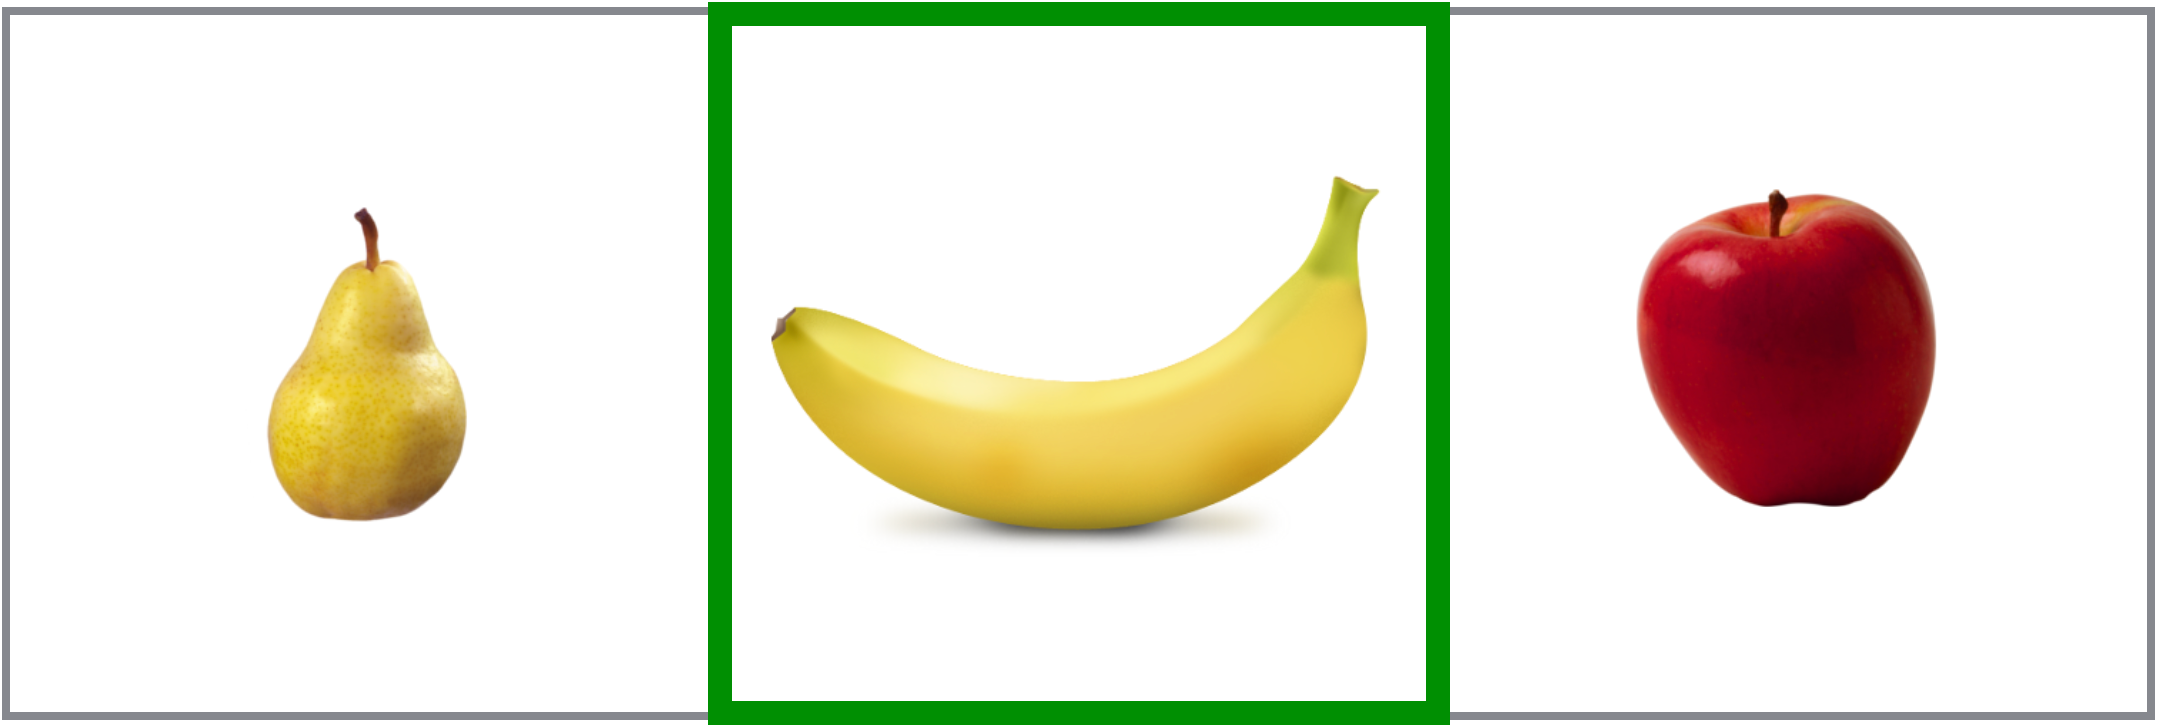
\includegraphics[width=\textwidth]{pics/banana-exampleyellow.png}
		\caption{Typical color.}
		\label{fig:bananayellow}
	\end{subfigure}
	\begin{subfigure}{.33\textwidth}
		\centering
		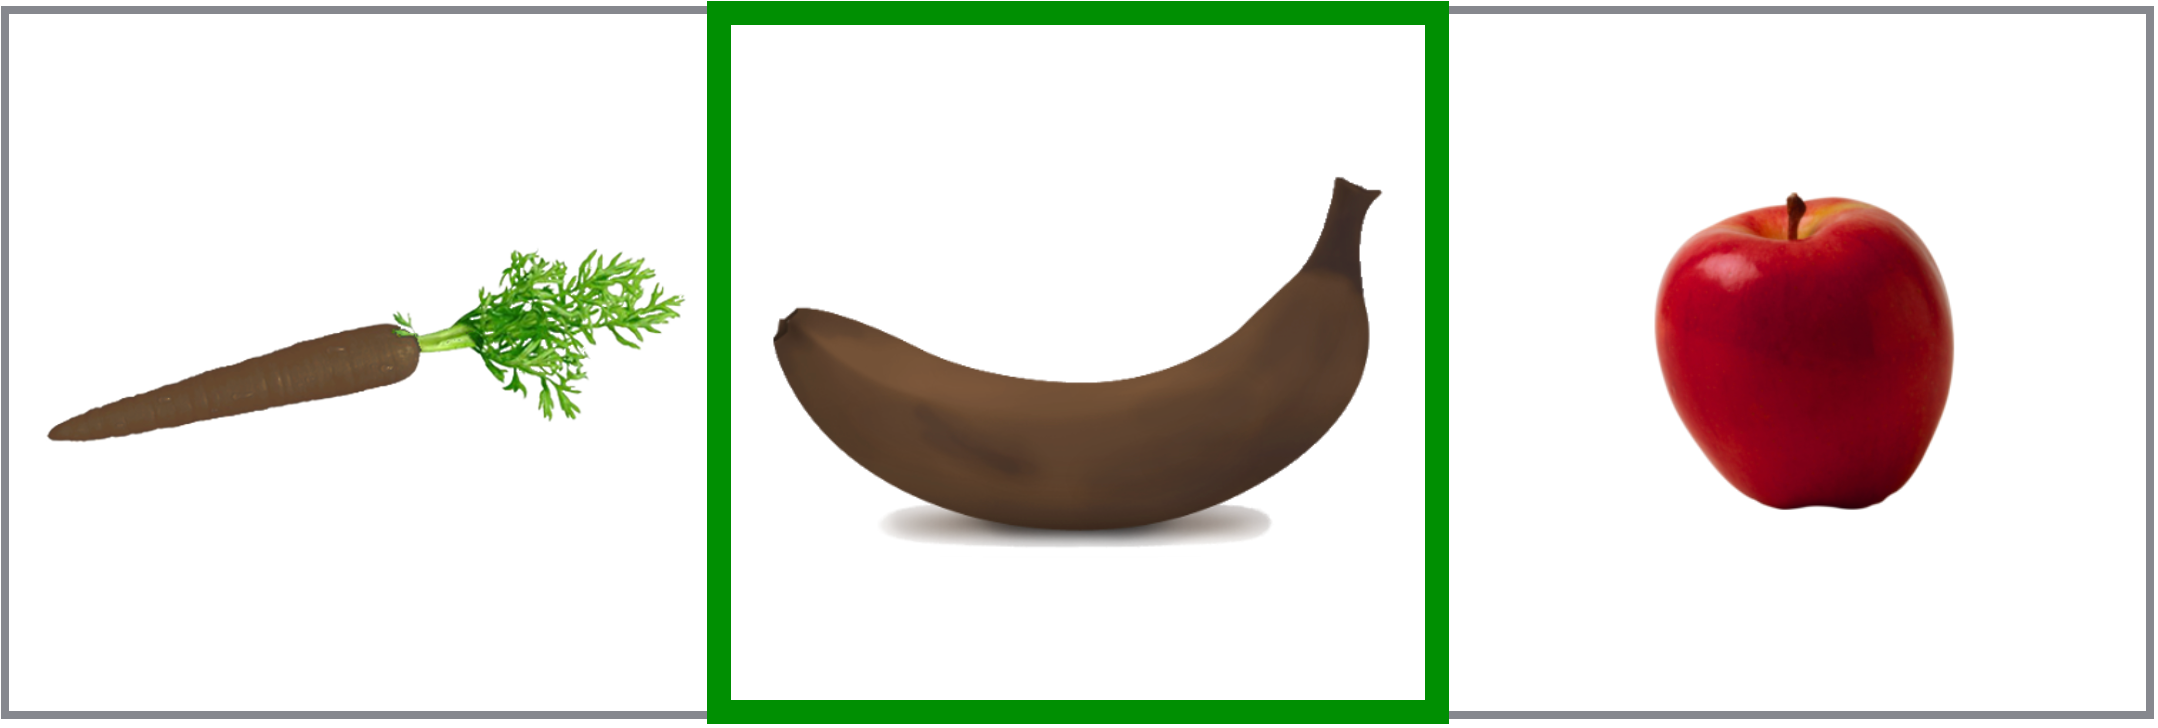
\includegraphics[width=\textwidth]{pics/banana-examplebrown.png}
		\centering
		\caption{Mid-typical color.}
		\label{fig:bananabrown}
	\end{subfigure}
	\begin{subfigure}{.33\textwidth}
		\centering
		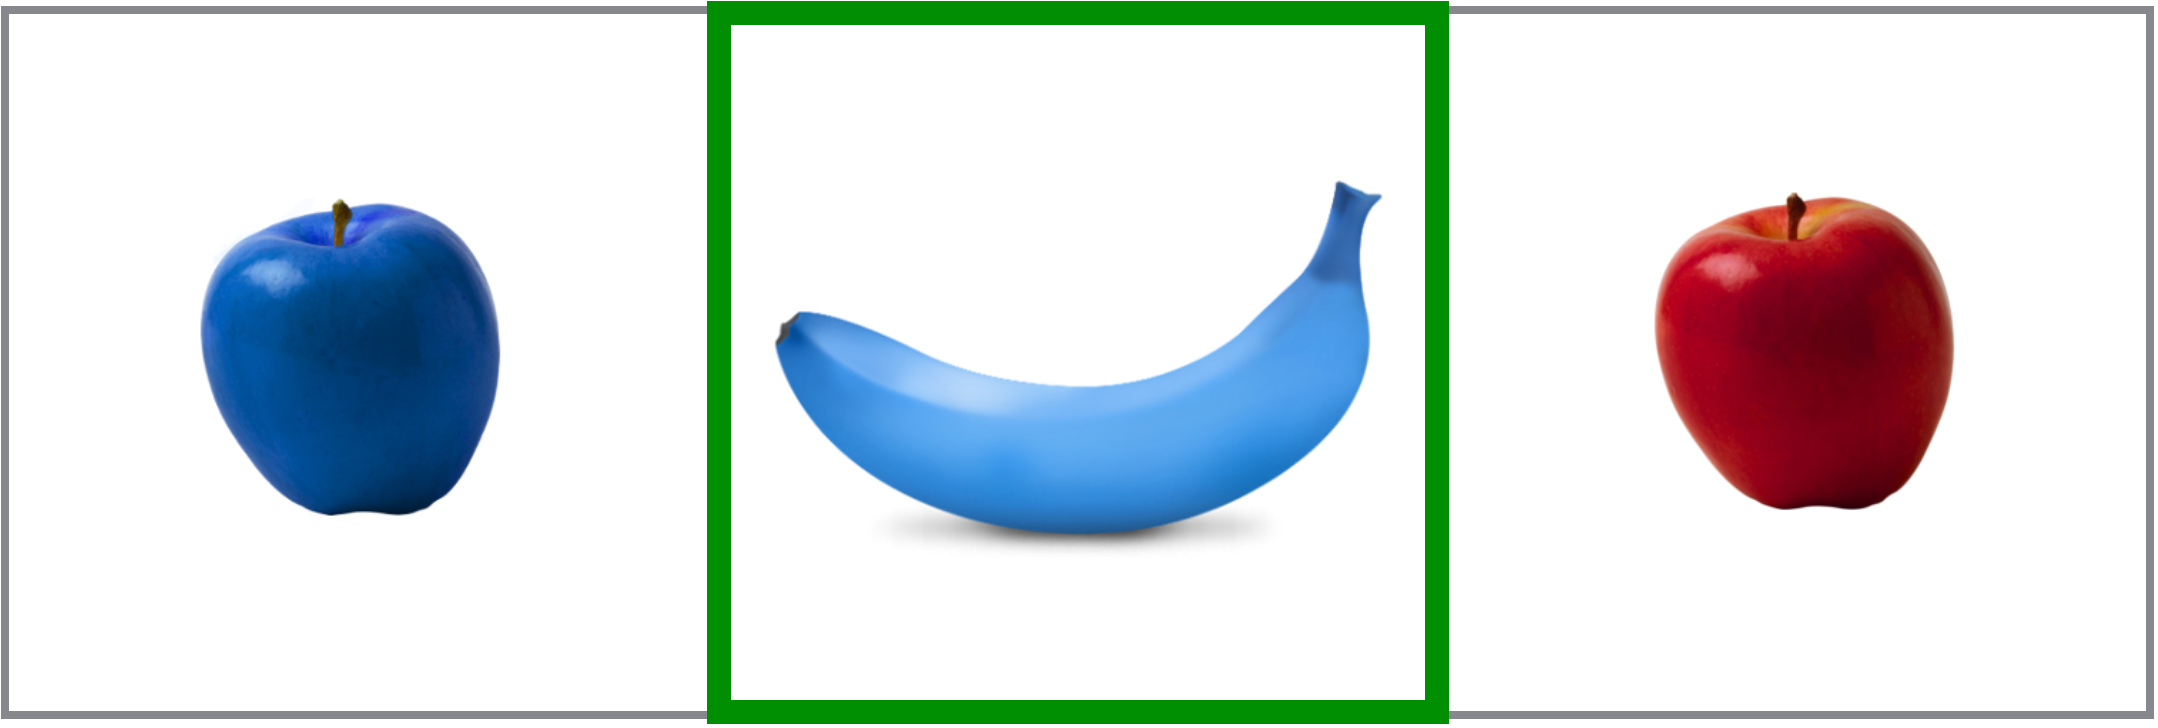
\includegraphics[width=\textwidth]{pics/banana-exampleblue.png}
		\caption{Atypical color.}
		\label{fig:bananablue}
	\end{subfigure}
	\caption{Three hypothetical contexts where color is redundant for referring to the target banana. Banana varies in typicality from left to right. Each context contains one distractor of the same color as the target, and one of a different color.}
	\label{fig:bananaexamples}
\end{figure}

\begin{table}
\centering
\caption{Hypothetical semantic values for utterances (rows) as applied to objects (columns).}
\begin{tabular}{l l l l l}
\toprule
 & yellow banana & brown banana & blue banana & other\\
\midrule
\emph{banana} & .9 & .35 & .1 & .015 \\
\midrule
\emph{yellow banana} & .99 & .015 & .015 & .015 \\
\emph{brown banana} & .015 & .99 & .015 & .015 \\
\emph{blue banana} & .015 & .015 & .99 & .015 \\
\midrule
other & .015 & .015 & .015 & .99 \\
\bottomrule
\end{tabular}
\label{tab:colorobjectfidelities}
\end{table}

Inputting these contexts and semantic values into the RSA model used thus far, with $\beta_i$ = 12 and $\beta_c$ = 5 (that is, both informativeness and utterance cost receive a substantial weight), the resulting speaker probabilities for the (minimal) \emph{banana} are .99, .37, and .05, to refer to the yellow banana, the brown banana, and the blue banana, respectively. In contrast, the resulting speaker probabilities for the redundant \emph{yellow banana}, \emph{brown banana}, and \emph{blue banana} are .01, .63, and .95, respectively. That is, redundant color mention increases with decreasing semantic value of the simple \emph{banana} utterance.

So far we have shown that continuous semantics RSA can capture typicality effects in principle if we assume that semantic values do not operate at the adjective type level but instead captures the typicality of an object for the (minimal and redundant) referring expressions. If an object is more typical for the redundant expression than for the minimal expression, then the bigger the difference in typicality, the greater the relative informativeness of the redundant expression, and the greater the probability of it being produced. 

This example is somewhat oversimplified. In practice, speakers sometimes mention an object's color without mentioning the noun. In the contexts presented in \figref{fig:bananaexamples} this does not make much sense because there is always a competitor of the same color present. In contrast, in the contexts in \figref{fig:condInf} and \figref{fig:condOverinf}, color alone disambiguates the target. This suggests that we should consider among the set of utterance alternatives not just the simple type mentions (e.g., \emph{banana}) and color-and-type mentions (e.g., \emph{yellow banana}), but also simple color mentions (e.g., \emph{yellow}). The dynamics of the model proceed as before.

We can now ask whether taking into account this more fine-grained notion of a continuous semantics affects the probability of redundantly mentioning color. Because the stimuli for Exp.~1 were specifically designed to be realistic objects with low color-diagnosticity, they do not include objects with low typicality values or large degrees of variation in typicality. This makes the dataset from Exp.~1 not well-suited for investigating typicality effects.\footnote{We did elicit typicality norms for the items in Exp.~1 and replicated the previously documented typicality effects on the four items that did exhibit variation in typicality. See \appref{sec:exp1typicality} for details.} We therefore conducted a separate production experiment in the same paradigm but with two broad changes: first, objects' color varied in typicality; and second, we did not manipulate object size, focusing only on color mention. This allows us to ask three questions: first, do we replicate the typicality effects reported in the literature -- that is, are less color-typical objects more likely to lead to redundant color use than more color-typical objects? Second, does RSA with empirically elicited typicality values as proxy for a continuous semantics capture speakers' behavior? Third, does the semantic value depend only on typicality, or is there still a role for modifier type level noise  of the kind we investigated in the previous section? In addition, we can investigate the extent to which utterance cost, which we found not to play a role in the previous section, affects the choice of referring expression.

%Additionally, the proposed RSA model allows us to ask questions that have not been addressed previously. In particular, it allows us to test for complex interactions of contextual informativeness of color and type, by manipulating both whether there is a distractor of the same type present and whether there is a distractor of the same color present. 


\subsection{Experiment 2: color typicality effects}
\label{sec:modifiertypicalityeffects}



\subsubsection{Method}

\paragraph{Participants}
We recruited 61 pairs of participants (122 participants total) over Amazon's Mechanical Turk who were each paid \$1.80 for their participation. 


\paragraph{Procedure}

The procedure was identical to that of Exp.~1. See \figref{fig:mturk} for an example speaker and listener perspective.


\begin{figure}[bt!]
	\centering
	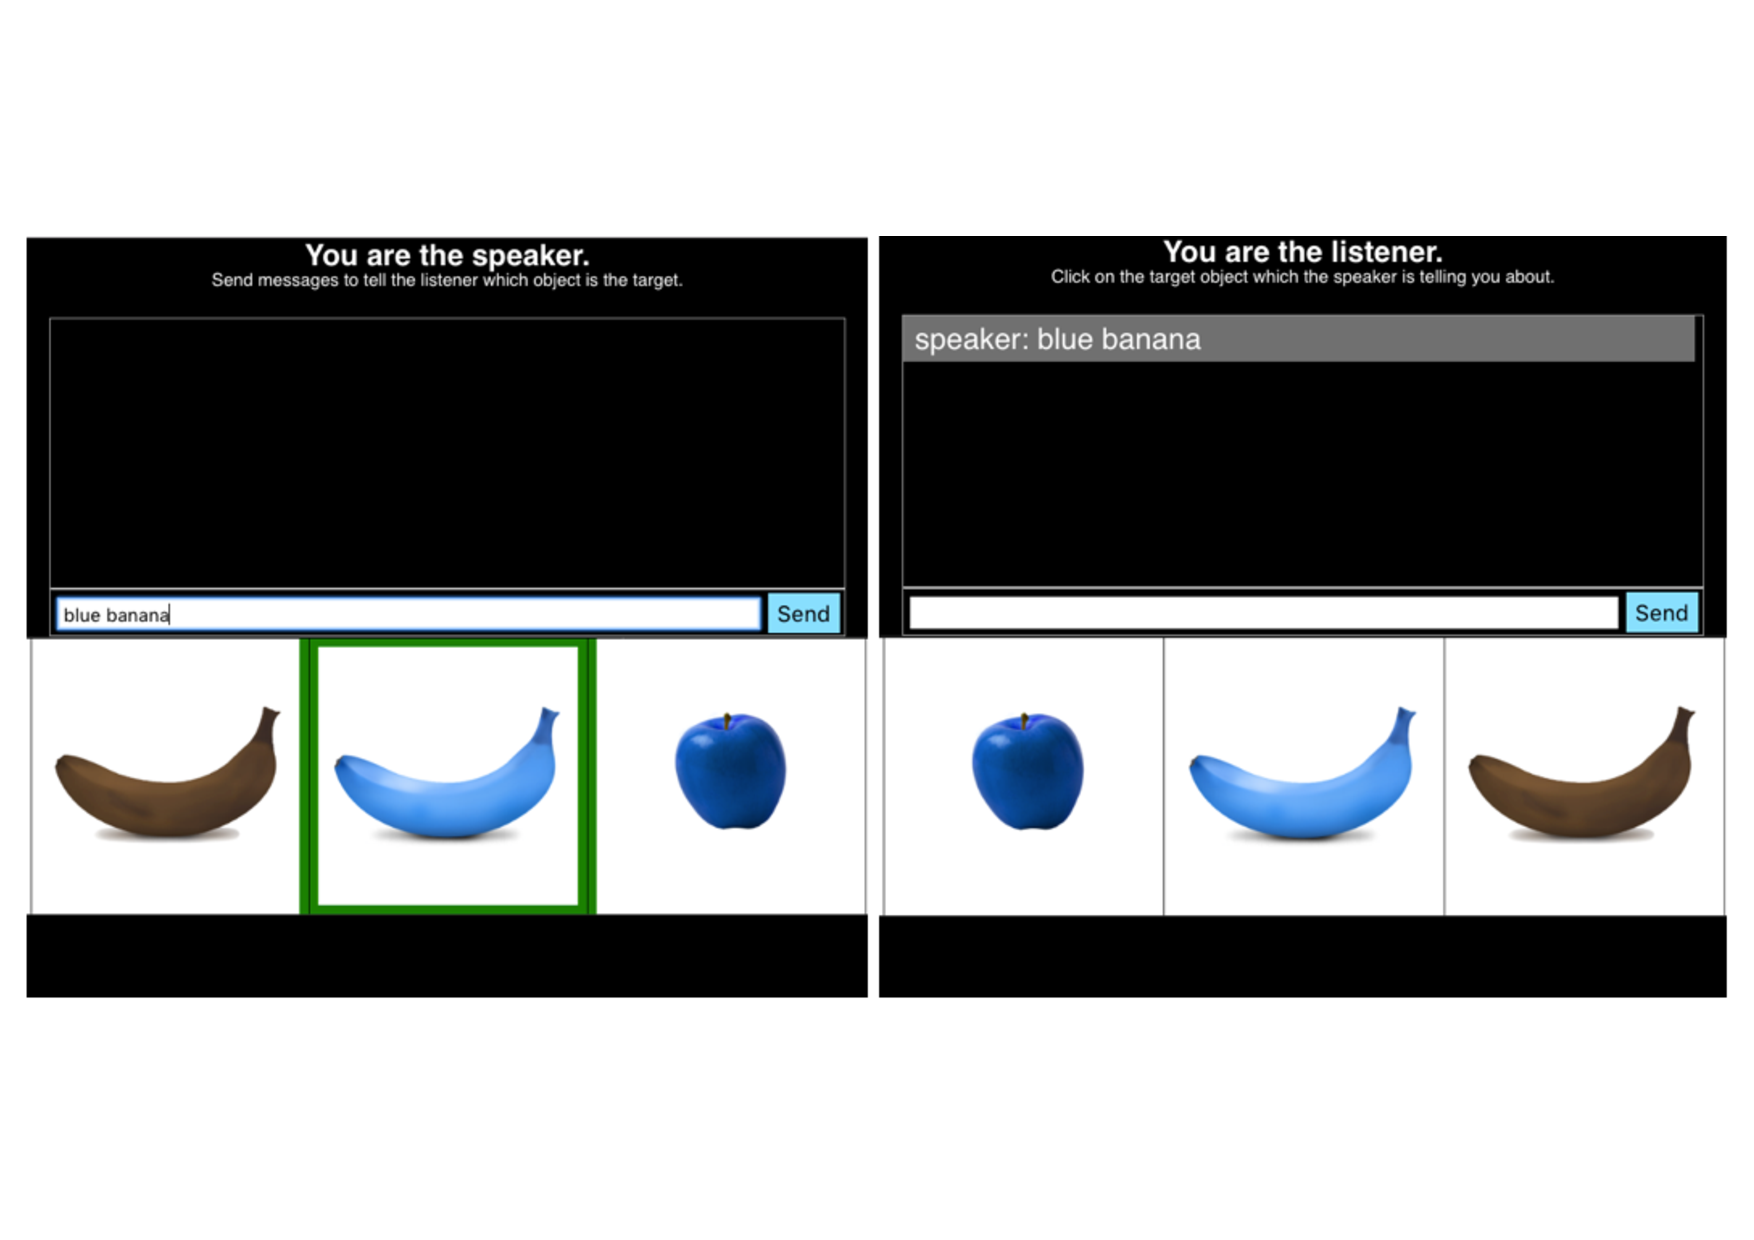
\includegraphics[width=1\textwidth]{pics/design_0}
	\caption{Example displays from the speaker's (left) and listener's (right) perspective in an informative-cc (i.e., presence of another object of the same type and one with the same color) condition.
	}
	\label{fig:mturk}
\end{figure}

\paragraph{Materials}

Each participant completed 42 trials. In this experiment, there were no filler trials, since pilot studies with and without fillers delivered very similar results. Each array presented to the participants consisted of three objects that could differ in type and color. One of the three objects functioned as a target and the other two as its distractors.

The stimuli were selected from seven color-diagnostic food items (apple, avocado, banana, carrot, pear, pepper, tomato), which all occurred in a typical, mid-typical and atypical color for that object. For example, the banana appeared in the colors yellow (typical), brown (midtypical), and blue (atypical). 
All items were presented as targets and as distractors. Pepper additionally occurred in a fourth color, which only functioned as a distractor due to the need for a green color competitor (as explained in the following paragraph). 

We refer to the different context conditions  as ``informative'', ``informative-cc'', ``overinformative'', and ``overinformative-cc'' (see \figref{fig:conditions}). A context was ``overinformative'' (\figref{fig:condOverinf}) when mentioning the type of the item, e.g., banana, was sufficient for unambiguously identifying the target.  In this condition, the target never had a color competitor. This means that mentioning color alone (without a noun) was also unambiguously identifying. In contrast, in the overinformative condition with a color competitor (``overinformative-cc'', \figref{fig:condOverinfcc}), color alone was not sufficient. In the informative conditions, color and type mention were necessary for unambiguous reference. Again, one context type did (\figref{fig:condInf}) and one did not (\figref{fig:condOverinfcc}) include a color competitor among its distractors.

\begin{figure}[bt!]
	% following line responsible for centered subfigure captions -- maybe don't do it
	% \captionsetup[subfigure]{justification=centering}
	\begin{subfigure}{.5\textwidth}
		\centering
		
\includegraphics[width=.8\textwidth]{pics/cond_inf.png}
		\caption{informative (without color competitor)}
		\label{fig:condInf}
	\end{subfigure}
	\begin{subfigure}{.5\textwidth}
		\centering
		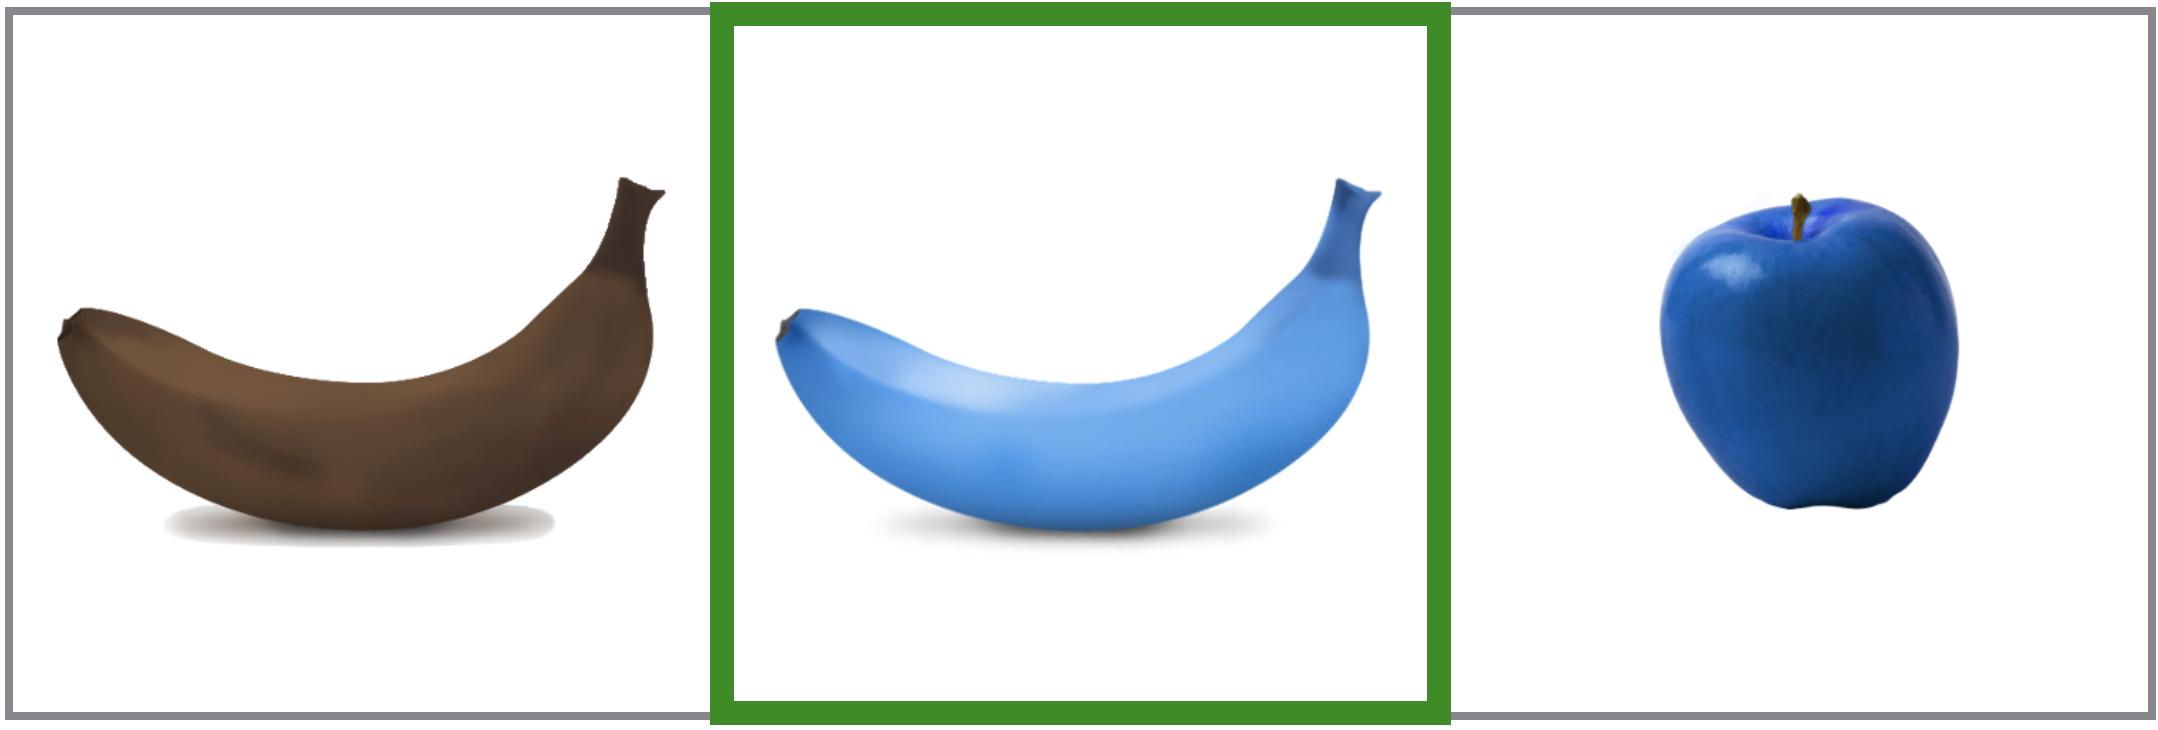
\includegraphics[width=.8\textwidth]{pics/cond_infcc.png}
		\centering
		\caption{informative-cc (with color competitor)}
		\label{fig:condInfcc}
	\end{subfigure}
	\begin{subfigure}{.5\textwidth}
		\centering
		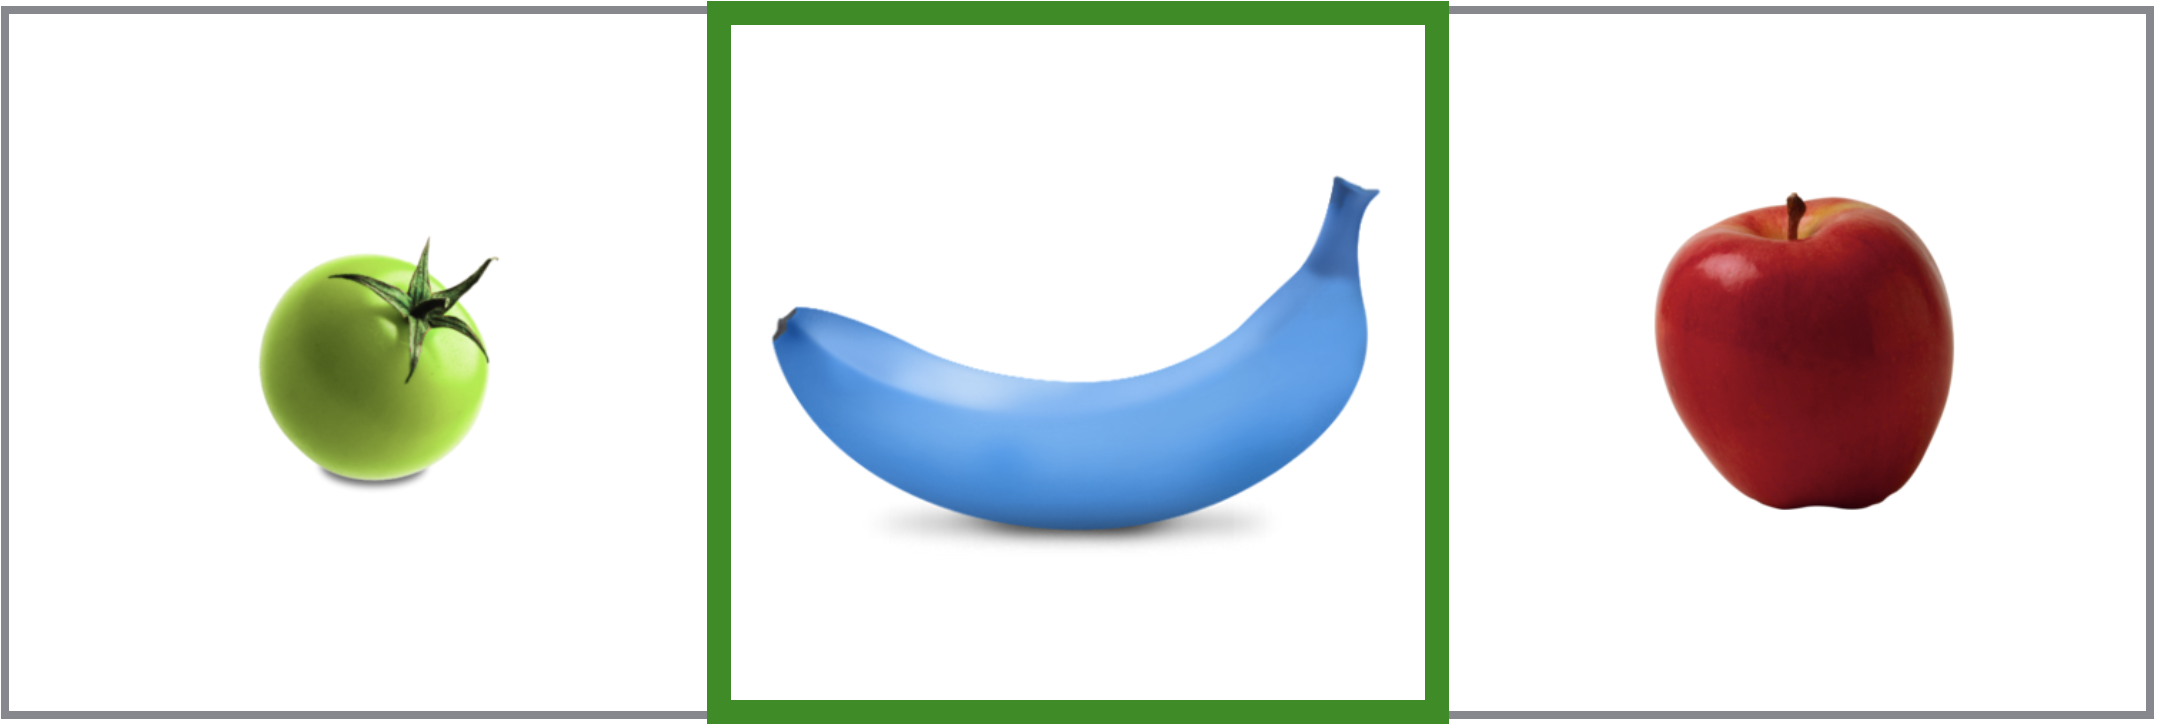
\includegraphics[width=.8\textwidth]{pics/cond_overinf.png}
		\caption{overinformative (without color competitor)}
		\label{fig:condOverinf}
	\end{subfigure}
	\begin{subfigure}{.5\textwidth}
		\centering
		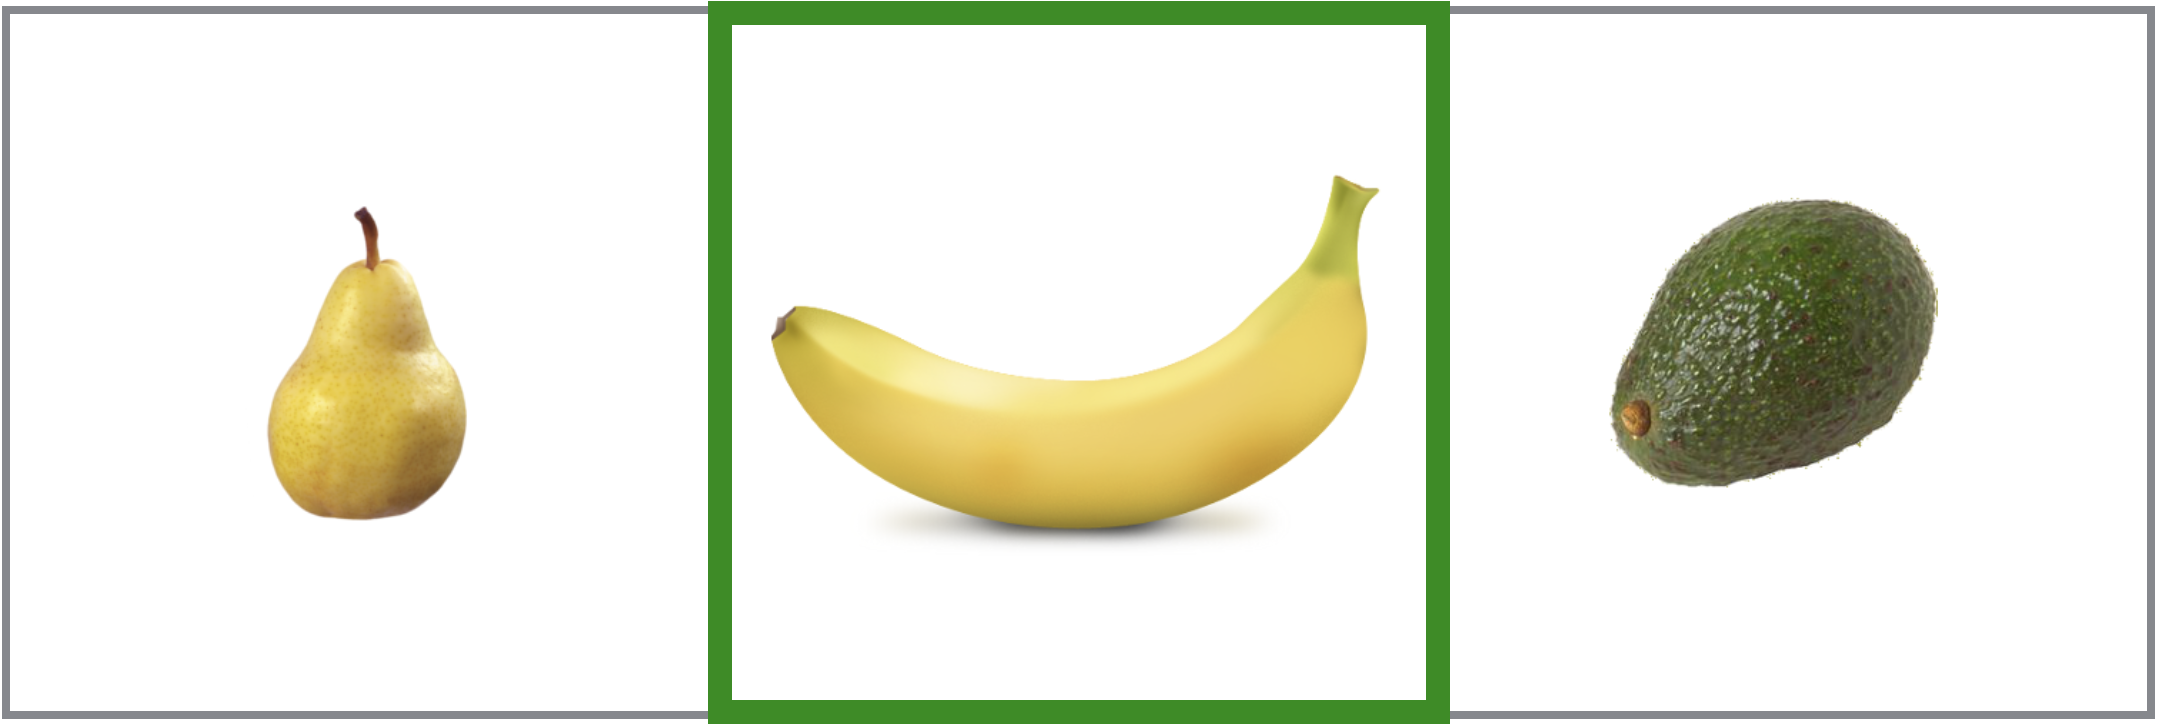
\includegraphics[width=.8\textwidth]{pics/cond_overinfcc.png}
		\centering
		\caption{overinformative-cc (with color competitor)}
		\label{fig:condOverinfcc}
	\end{subfigure}
	\caption{Examples of the four different context conditions in Exp.~2. They differed in the presence of an object of the same type (informative vs.~overinformative) and in the presence of another object of the same color as the target (with color competitor vs.~without color competitor). The green border marks the intended referent.}
	\label{fig:conditions}
\end{figure}

Each participant saw 42 different contexts. Each of the 21 items (color-type combinations) was the target exactly twice, but the context in which they occurred was drawn randomly from the four possible conditions mentioned above. In total, there were 84 different possible configurations (seven target food items, each of them in three colors, where each could occur in four contexts). Trial order was randomized.


\subsubsection{Data pre-processing and exclusion}

Two participant-pairs were excluded because they did not finish the experiment and therefore could not receive payment. Trials on which the speaker did not produce any utterances were also excluded, resulting in the exclusion of two additional participant-pairs.
Finally, there were 10 speakers who consistently used roundabout descriptions instead of direct referring expressions (e.g., \emph{monkeys love\dots} to refer to banana). These pairs were also excluded.

We analyzed data from 1974 trials. Just as in Exp.~1, participants communicated freely, which led to a vast amount of different referring expressions. To test the model's predictions, the utterance produced for each trial was classified as belonging to one of the following categories: \textit{type-only} (``banana''), \textit{color-and-type} (``yellow banana''), and \textit{color-only} (``yellow'') utterances. Referring expressions that included categories (``yellow fruit''), descriptions (``has green stem''), color-circumscriptions (``funky carrot''), and negations (``yellow but not banana'') were regarded as \textit{other} and excluded. To this end we conducted the following semi-automatic data pre-processing.
%Only five utterances (0.003\%) were assigned to the category "other".\\

The referring expressions were analyzed similarly to Exp.~1. First, 32 trials (1.6\%) were excluded because the listener selected the wrong referent. 109 trials (5.6\%) were excluded because the referring expressions included one of the exceptional cases described above (e.g., using negations). 
An R script then automatically checked the remaining 1833 utterances for whether they contained a precoded color term (i.e. \emph{green, purple, white, black, brown, yellow, orange, blue, pink, red, grey}) or type (i.e. \emph{apple, banana, carrot, tomato, pear, pepper, avocado}). This way, 96.5\% of the remaining cases were classified as mentioning type and/or color. 

However, this did not capture that sometimes, participants produced meaning-equivalent modifications of color/type terms for instance by adding suffixes (e.g., \emph{pinkish}), using abbreviations (e.g., \emph{yel} for \emph{yellow}), or using non-precoded color and type labels (e.g., \emph{lavender} or \emph{jalapeno}). In addition, expressions that contained a typo (e.g., \emph{blakc} instead of \emph{black}) could also not be classified automatically. One of the authors (EK) therefore manually hand-coded these cases.
% Most of the time, participants converged on a convention of producing only the target's size and/or color, e.g., \emph{purple} or \emph{big blue}, but not an article (e.g., \emph{the}) or the noun corresponding to the object's type  (e.g., \emph{comb}). Articles were omitted in 93.1 \% of cases and nouns were omitted in 71.5 \% of cases. We did not analyze this any further.

There were 6 cases (0.3\%) that could not be categorized. Those were mostly greetings (e.g.,\emph{Hi}), other comments (e.g., \emph{I have instructions to follow sometimes}) and not certainly identifiable utterances (e.g., \emph{re}). These were excluded. After exclusion, 1827 cases classified as one of \emph{color}, \emph{type}, or \emph{color-and-type} entered the analysis.


\subsubsection{Typicality norming}
\label{sec:typicalitynormingcolor}

In order to test for typicality effects on the production data and to evaluate RSA's performance, we collected empirical typicality values for each utterance/object pair (as proxy for values of the sort listed in \tableref{tab:colorobjectfidelities}) across three separate studies. The first study collected typicalities for \emph{color-and-type}/object pairs (e.g., \emph{yellow banana} as applied to a yellow banana, a blue banana, an orange pear, etc., see \figref{fig:colorobj}). The second study collected typicalities for \emph{type-only}/object pairs (e.g., \emph{banana} as applied to a yellow banana, a blue banana, an orange pear, etc., \figref{fig:obj}). The third study collected typicalities for \emph{color}/color pairs (e.g., \emph{yellow} as applied to a color patch of the average yellow from the yellow banana stimulus or to a color patch of the average orange from the orange pear stimulus, and so on, for all other colors, \figref{fig:colorpatch}). 

On each trial, participants saw one of the stimuli used in the production experiment in isolation and were asked: ``How typical is this object for a \emph{utterance}'', where \emph{utterance} was replaced by an utterance of interest. In the color typicality study, they were asked ``How typical is this color for the color \emph{color}?'', where \emph{color} was replaced by one of the relevant color terms. They then adjusted a continuous sliding scale with endpoints labeled ``very atypical'' and ``very typical'' to indicate their response. An overview of the differences between the three typicality norming studies is shown in Table~\ref{tab:normingoverview}. 

\begin{figure}[bt!]
	\subcaptionbox{color-and-type norming. \label{fig:colorobj}} {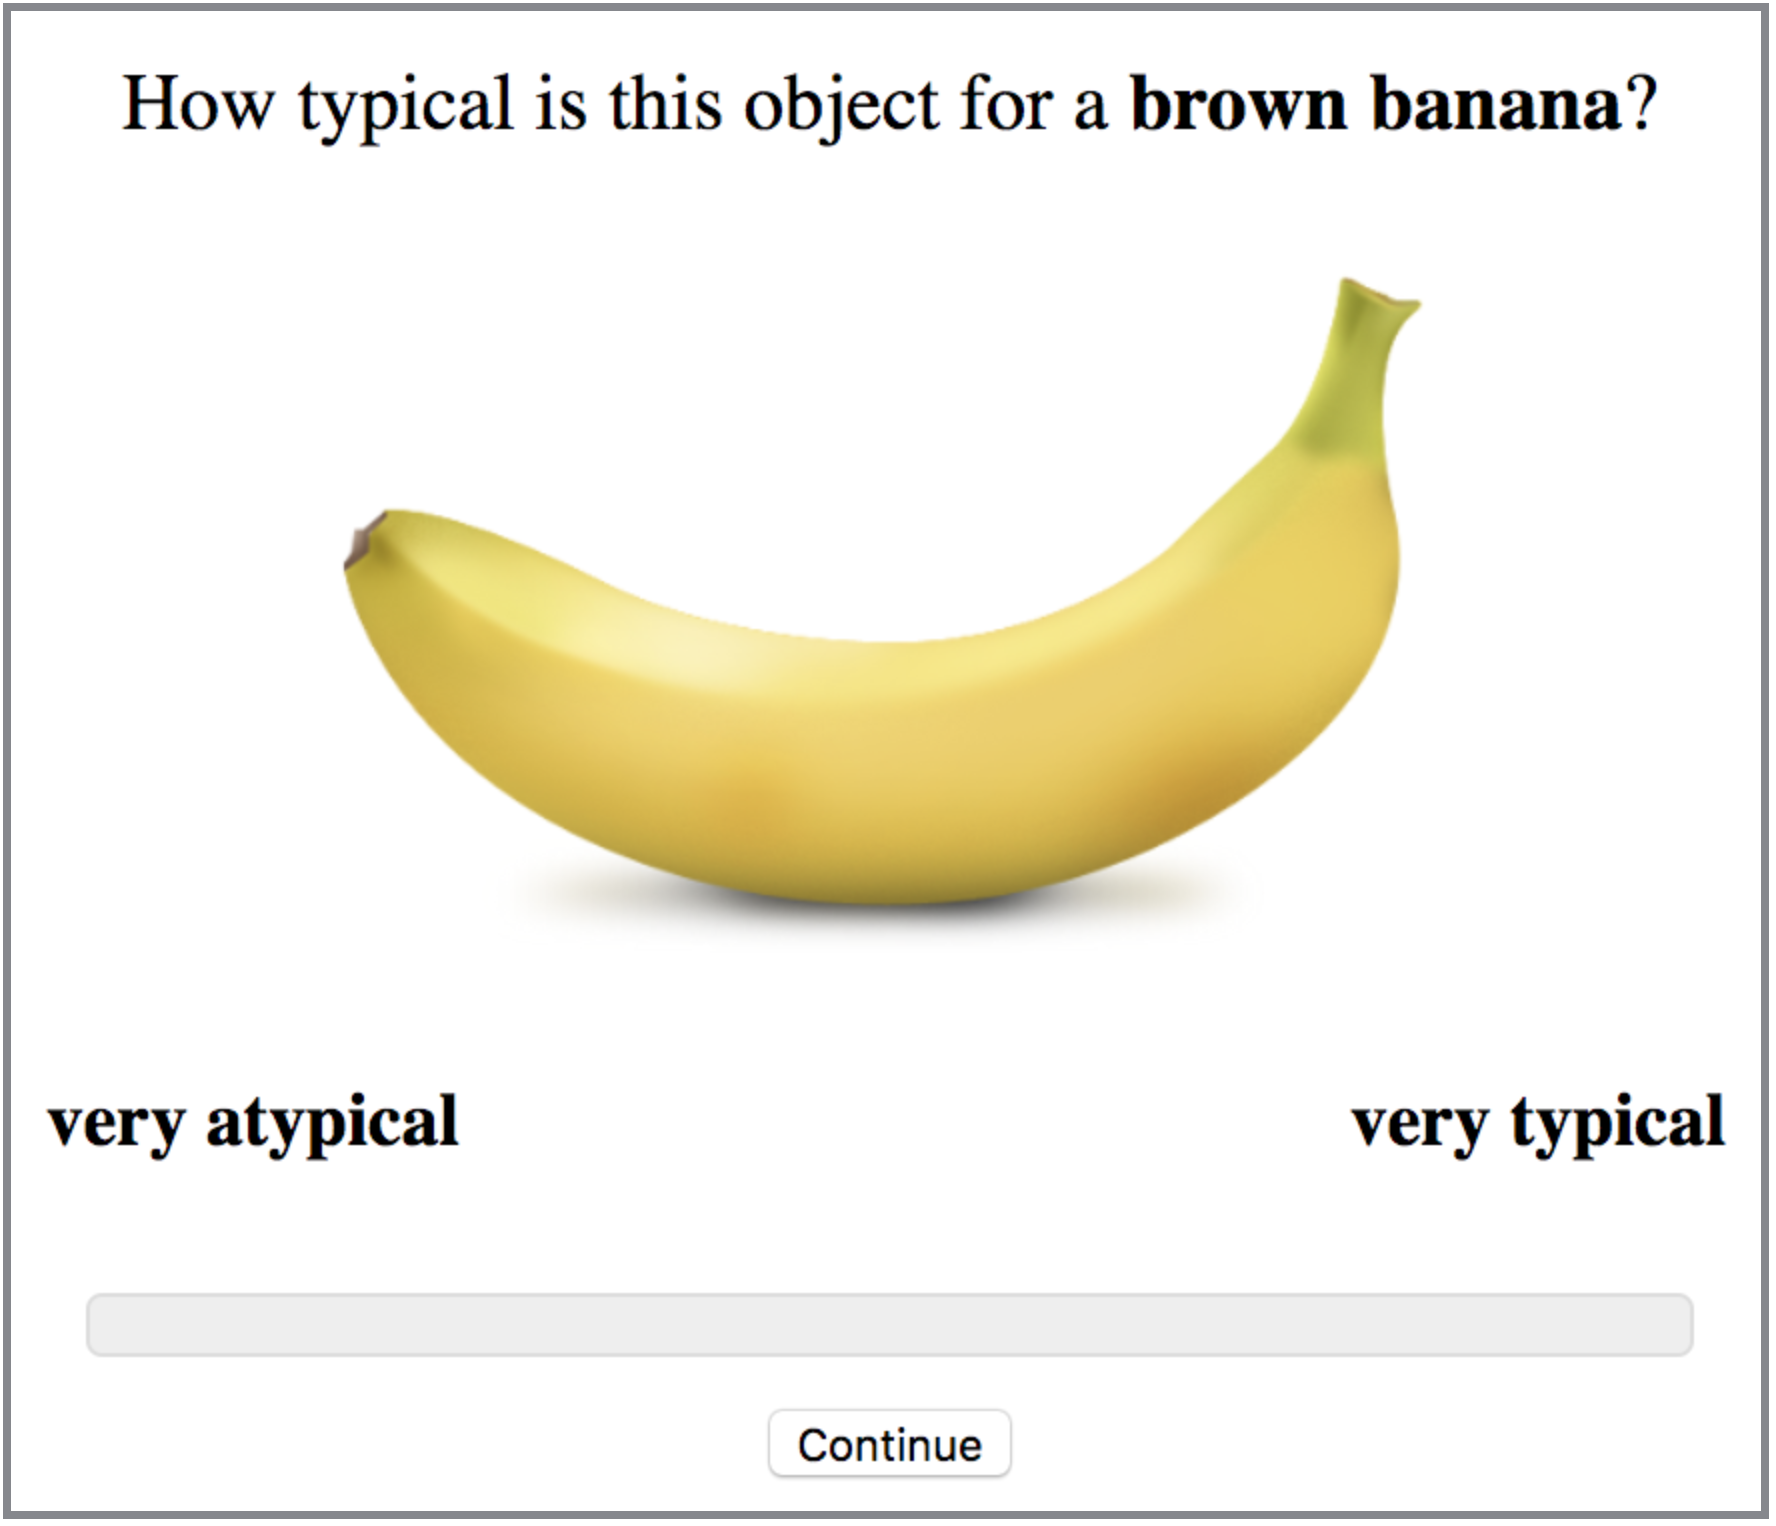
\includegraphics[width=2.1in]{pics/typnorm_colorobj}} \hfill
	\subcaptionbox{type-only norming. \label{fig:obj}} 
	{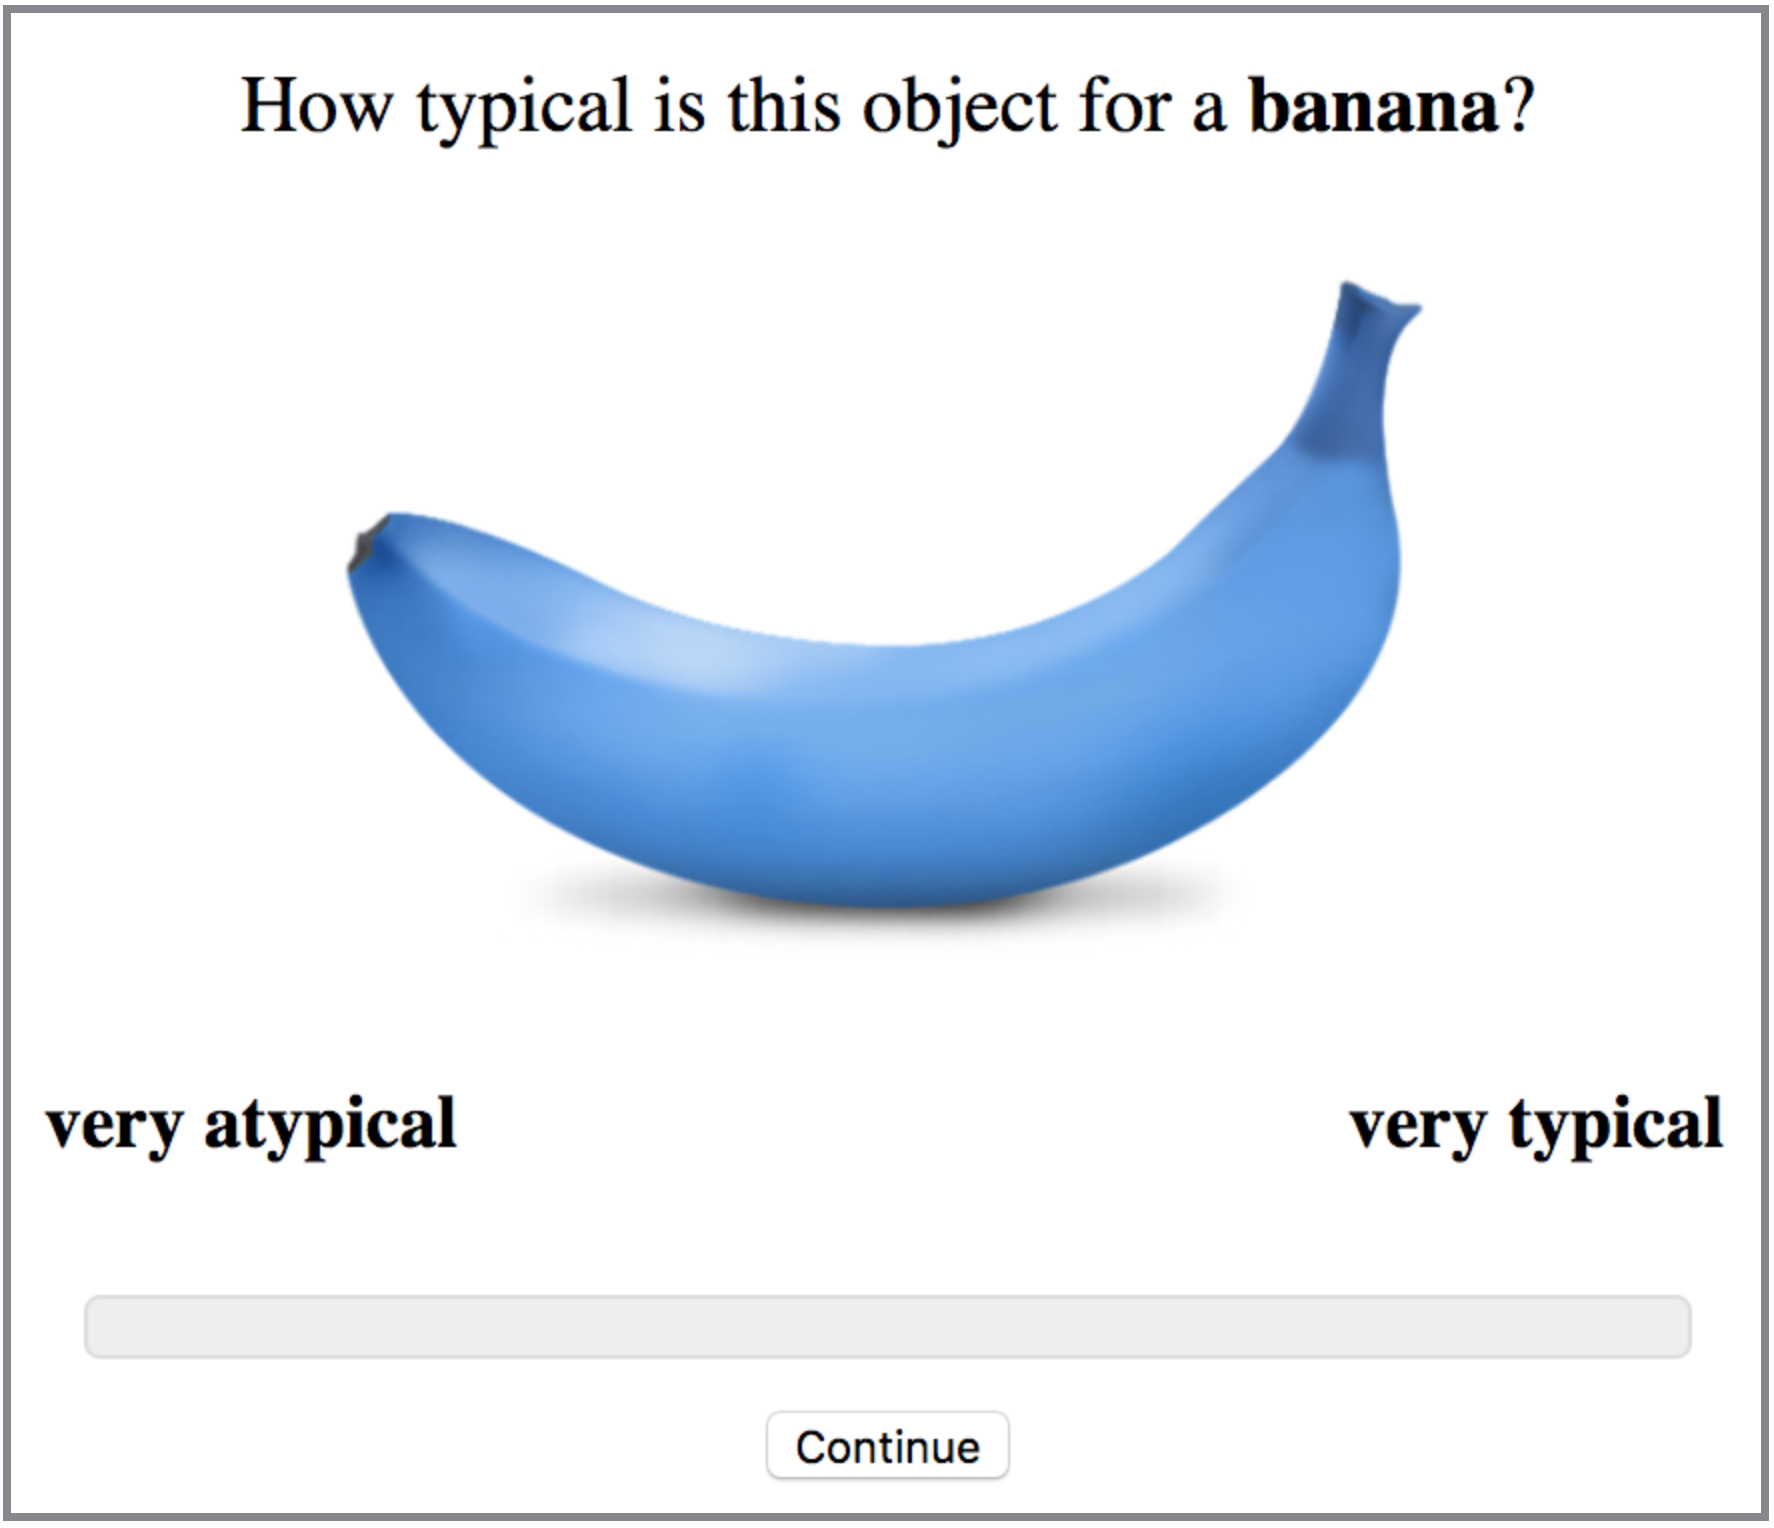
\includegraphics[width=2in]{pics/typnorm_obj}} \hfill
	\subcaptionbox{color-only norming. \label{fig:colorpatch}} {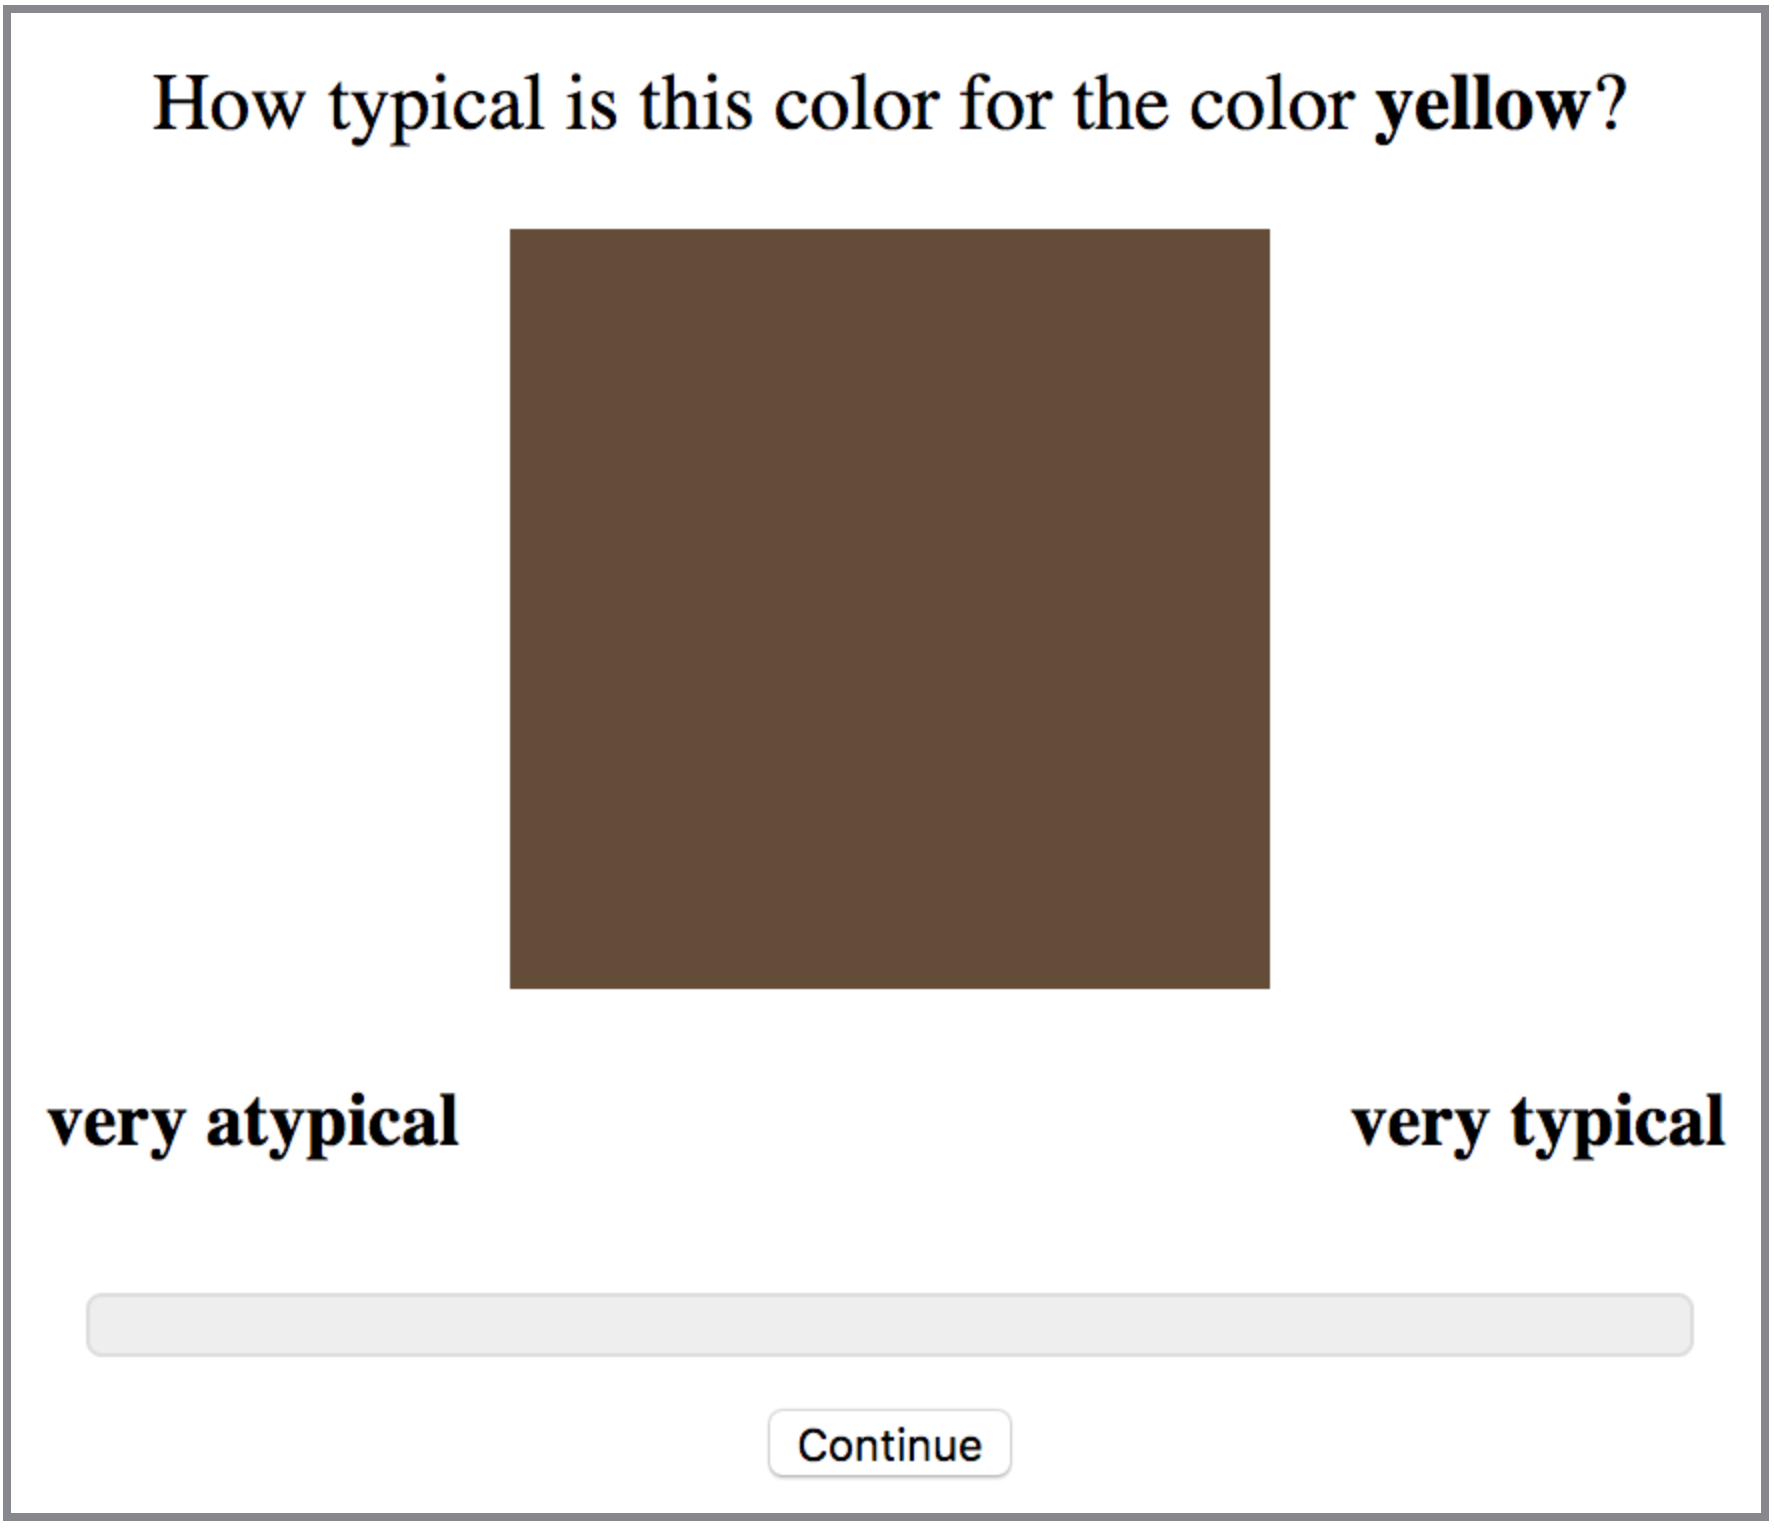
\includegraphics[width=2in]{pics/typnorm_colorpatch}}%
	\caption{Example stimuli exemplifying the three different typicality norming studies.}
	\label{fig:typ_norm}
\end{figure}

\begin{table}[bt!]
	\begin{tabular}{l l l l l l l}
		\toprule
		Utterances & Example & Images & Participants & Trials & Items & Excluded Participants\\
		\midrule
		Adj Noun & \emph{yellow banana} & object & 174 & 110 & 484 & 14\\ 
		Noun & \emph{banana} & object & 75 & 90 & 154 (198) & 1\\
		Adj & \emph{yellow} & color patch & 110 & 90 & 176 (198) & None\\
		\bottomrule
	\end{tabular}
	\vspace{2mm}
	\caption{Overview of the typicality norming studies for Exp.~2. Items column contains the number of unique utterance-object pairs that we elicited responses for. The value in parentheses represents the number of items including utterances \textit{fruit}, \textit{vegetable}, \textit{cup} and \textit{pink}, which were not analyzed further.}
	\label{tab:normingoverview}
\end{table}

\begin{table}[bt!]
	\caption{Mean typicalities for banana items. Combinations where deterministic semantics would return TRUE are marked in boldface.}
\centering
	\begin{tabular}{r r r r r}
		\toprule
		%Utterance & Item & Typicality\\
		& \multicolumn{3}{c}{Banana items} & Other \\
		Utterance & yellow & brown  & blue & \\ 
		\midrule
		\emph{banana} & \textbf{.98} & \textbf{.66} & \textbf{.42} & .05  \\
		\midrule
		\emph{yellow banana} & \textbf{.97} & .30 & .15 & .05 \\
		\emph{brown banana} & .22 & \textbf{.91} & .15 & .04\\
		\emph{blue banana} & .16 & .15 & \textbf{.92} & .06\\
		\bottomrule
	\end{tabular}
	\vspace{5mm}
	\label{tab:bananatypicalities}
\end{table}

Slider values were coded as falling between 0 (`very atypical') and 1 (`very typical'). 
For each utterance-object combination, we computed mean typicality ratings. The means for the banana items are shown in \tableref{tab:bananatypicalities}. The values are very similar to those hypothesized for the purpose of the example in \tableref{tab:colorobjectfidelities}. The means for all items are visualized in \figref{fig:exp2colortypicalitymeans}.

\begin{figure}
	\centering
	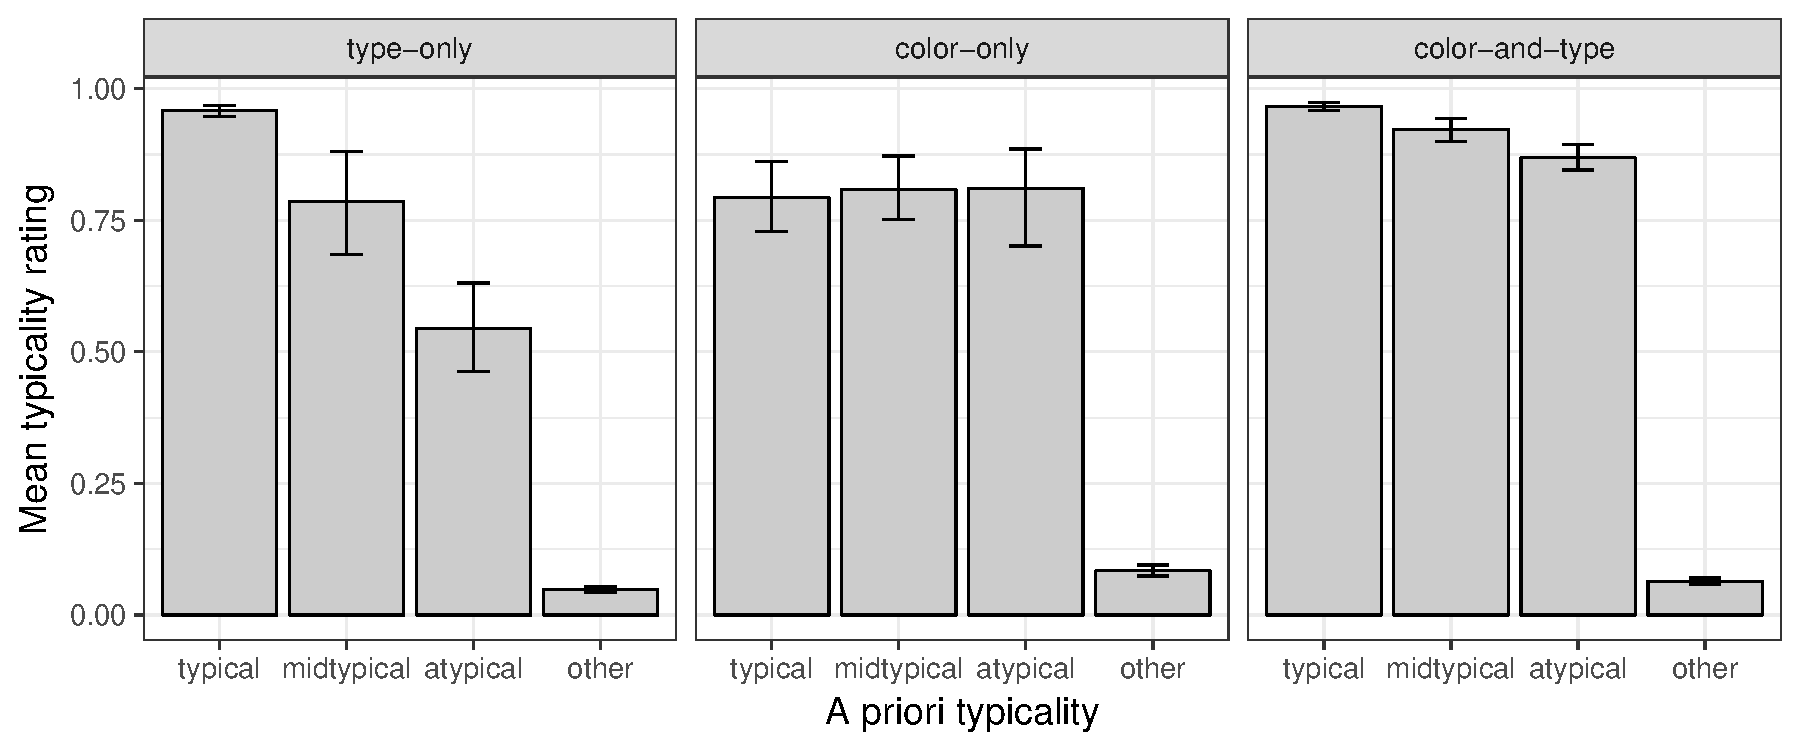
\includegraphics[width=\textwidth]{pics/exp2colortypicalitymeans.pdf}
	\caption{Mean typicality ratings for the three norming studies (type-only, color-only, color-and-type). The results are categorized according to the objects' a priori typicality as determined by the experimenters (yellow banana = typical, brown banana = midtypical, blue banana = atypical). The category \emph{other} comprises all utterance-object combinations where a Boolean semantics would return false. Error bars indicate bootstrapped 95\% confidence intervals.}
	\label{fig:exp2colortypicalitymeans}
\end{figure}

The typicality elicitation procedure we employed here is somewhat different from that employed by \citeA{Westerbeek2015}, who asked their participants ``How typical is this color for this object?'' We did this for conceptual reasons: the values that go into the semantics of the RSA model are most easily conceptualized as the typicality of an object as an instance of an utterance, rather than as the degree to which an object's color is representative of that object. While the typicality of a feature for an object type no doubt plays into how good of an instance of the utterance the object is, deriving our typicalities from the  statistical properties of the distributions of features in objects is beyond the scope of this paper. We expect, however, that the simple \textsc{Type}-object typicalities most closely approximates the Westerbeek question because the employed objects are color-diagnostic -- asking whether a blue or a yellow banana is a typical \textit{banana} is similar to asking whether or not the bananas' most salient property -- their color -- is typical.\footnote{See also \appref{sec:exp1typicality} for an independent comparison of our question and the Westerbeek question as applied to typicality norms for the items in Exp.~1. In general, the \textsc{Type}-object values are highly correlated with the Westerbeek question values.} 

Mean typicality values obtained in the norming studies are used in the analyses and visualizations in the following.

\subsubsection{Results and discussion}

Proportions of type-only (\emph{banana}), color-and-type (\emph{yellow banana}), color-only (\emph{yellow}), and other (\emph{funky carrot}) utterances are shown in \figref{fig:exp2empirical} as a function of the described item's mean type-only (\emph{banana}) typicality. Visually inspecting just the explicitly marked \emph{yellow banana}, \emph{brown banana}, and \emph{blue banana} cases suggests a large typicality effect in the overinformative conditions as well as a smaller typicality effect in the informative conditions, such that color is less likely to be produced with increasing typicality of the object. 

\begin{figure}
\centering
	\begin{subfigure}{.85\textwidth}
		\centering
		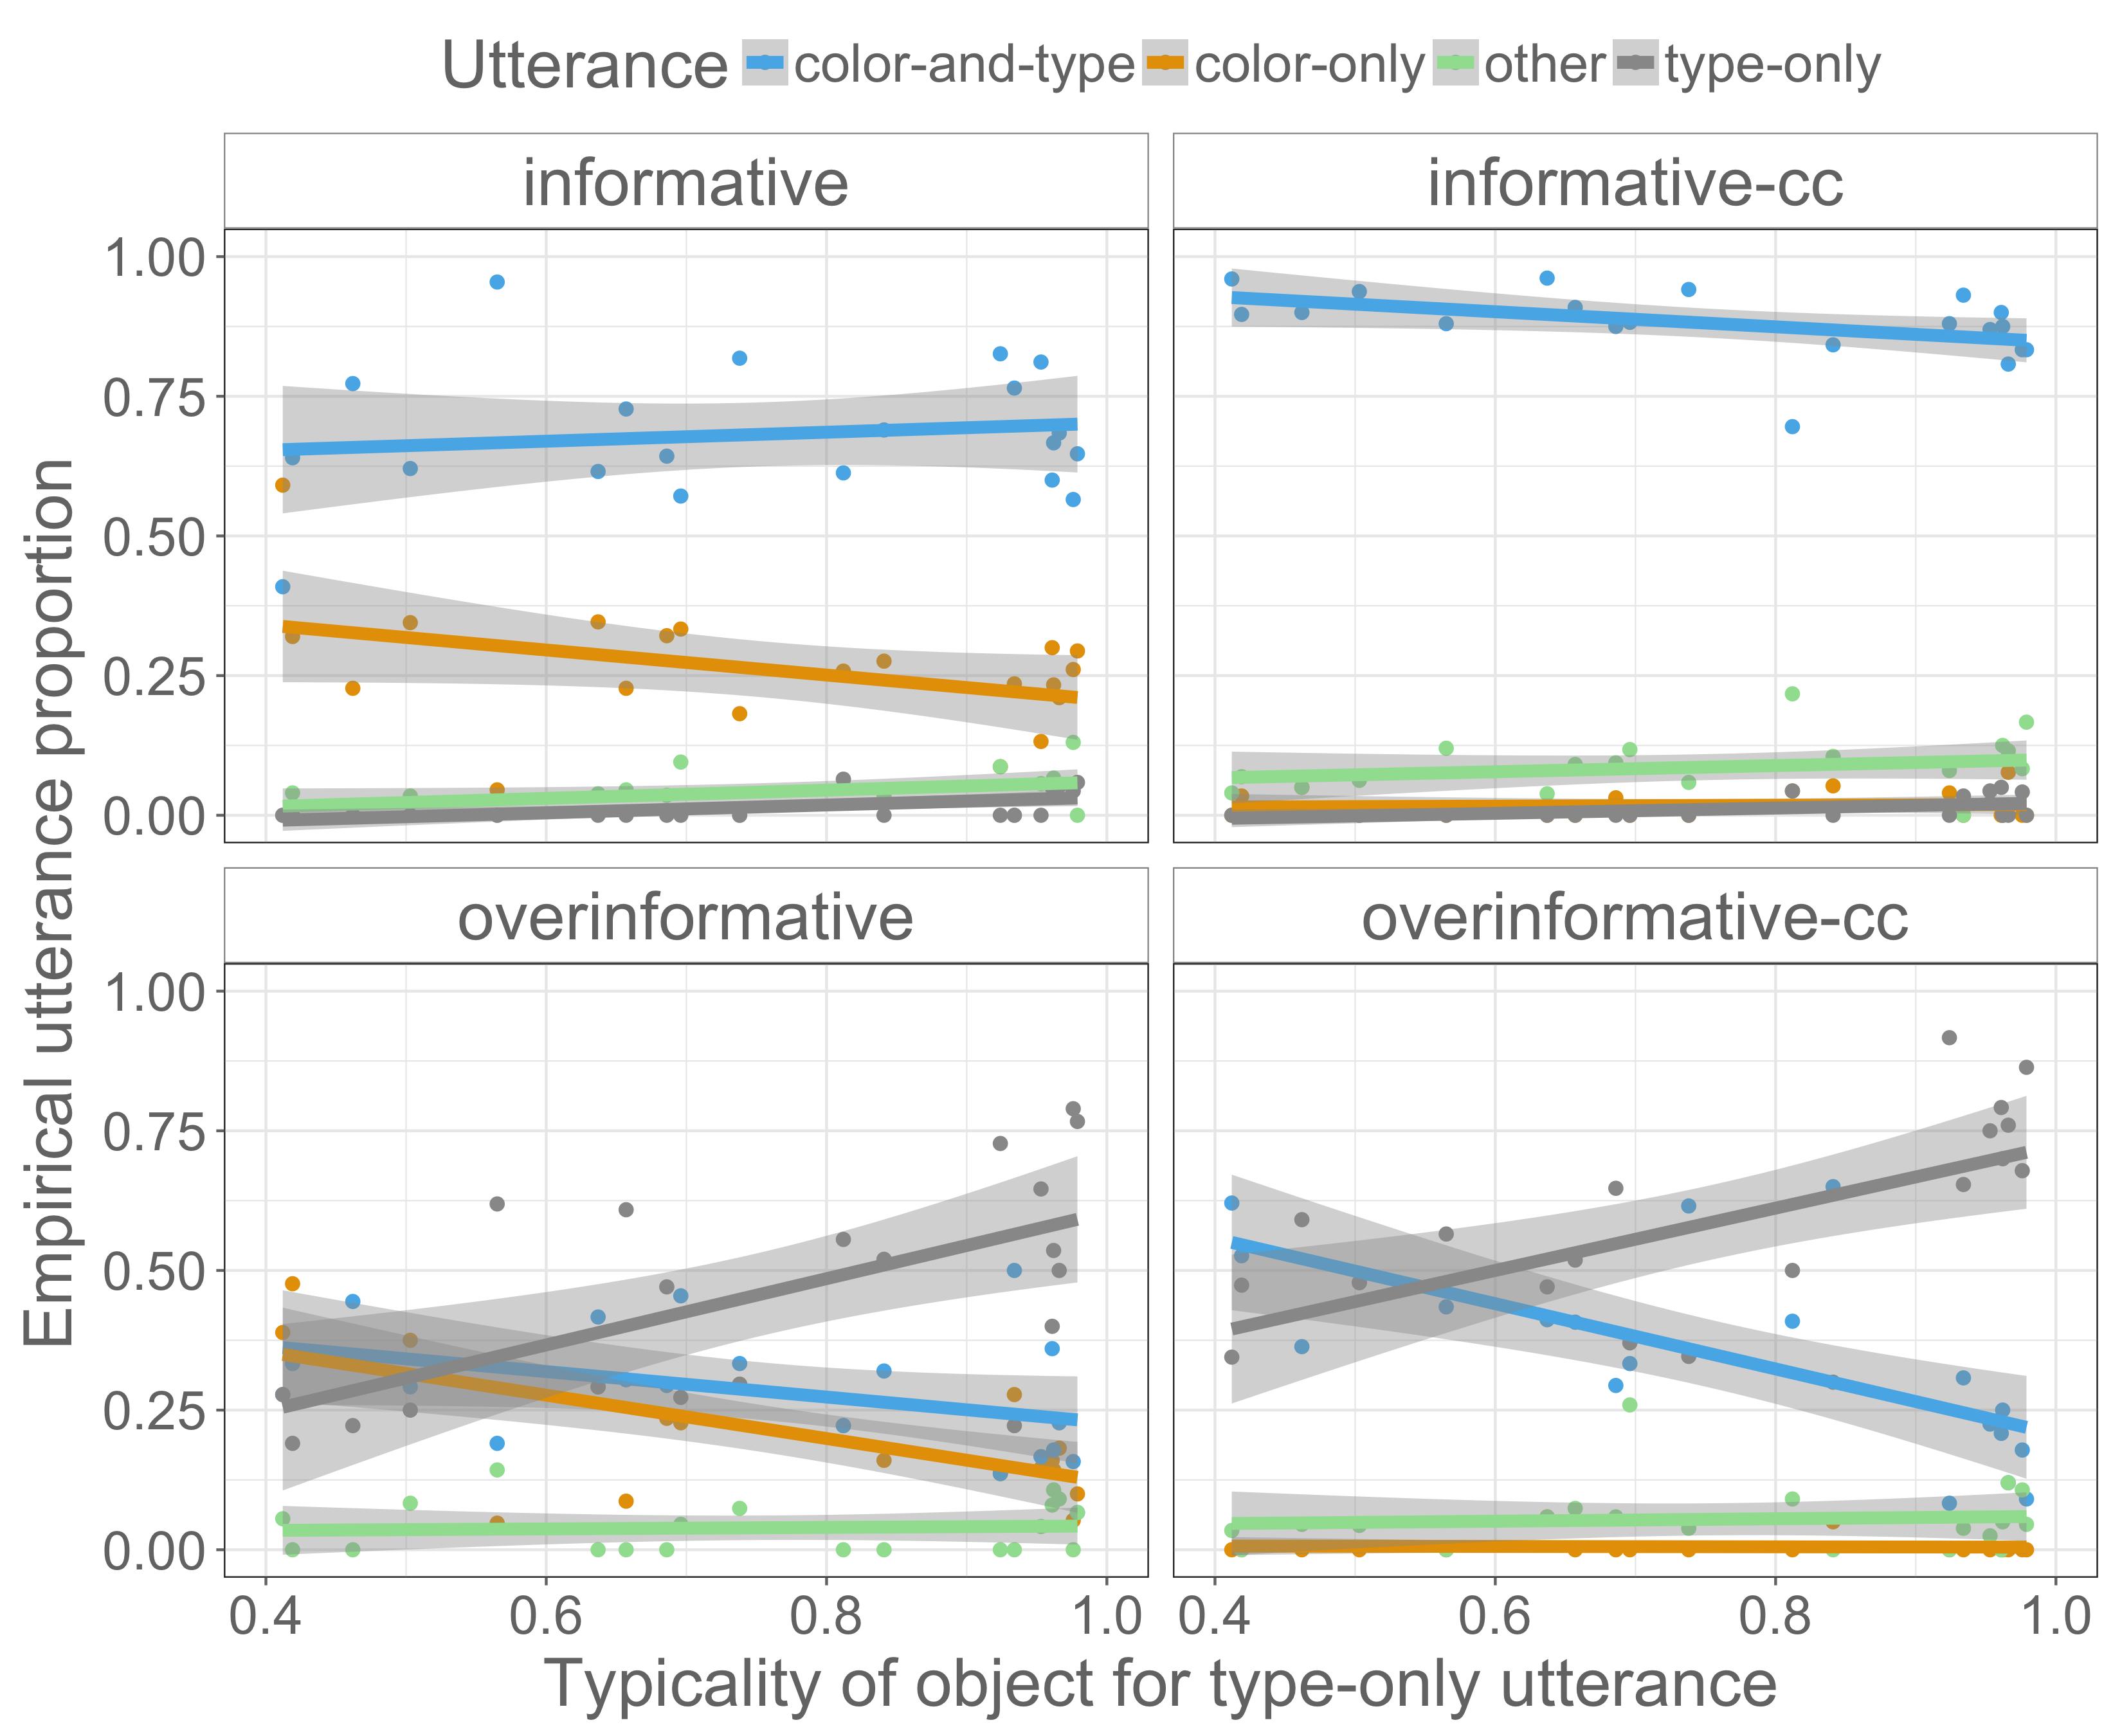
\includegraphics[width=.8\textwidth]{pics/empiricalProportions_typ.png}
		\caption{Empirical utterance proportions}
		\label{fig:exp2empirical}
	\end{subfigure}
	
	\begin{subfigure}{.85\textwidth}
		\centering
		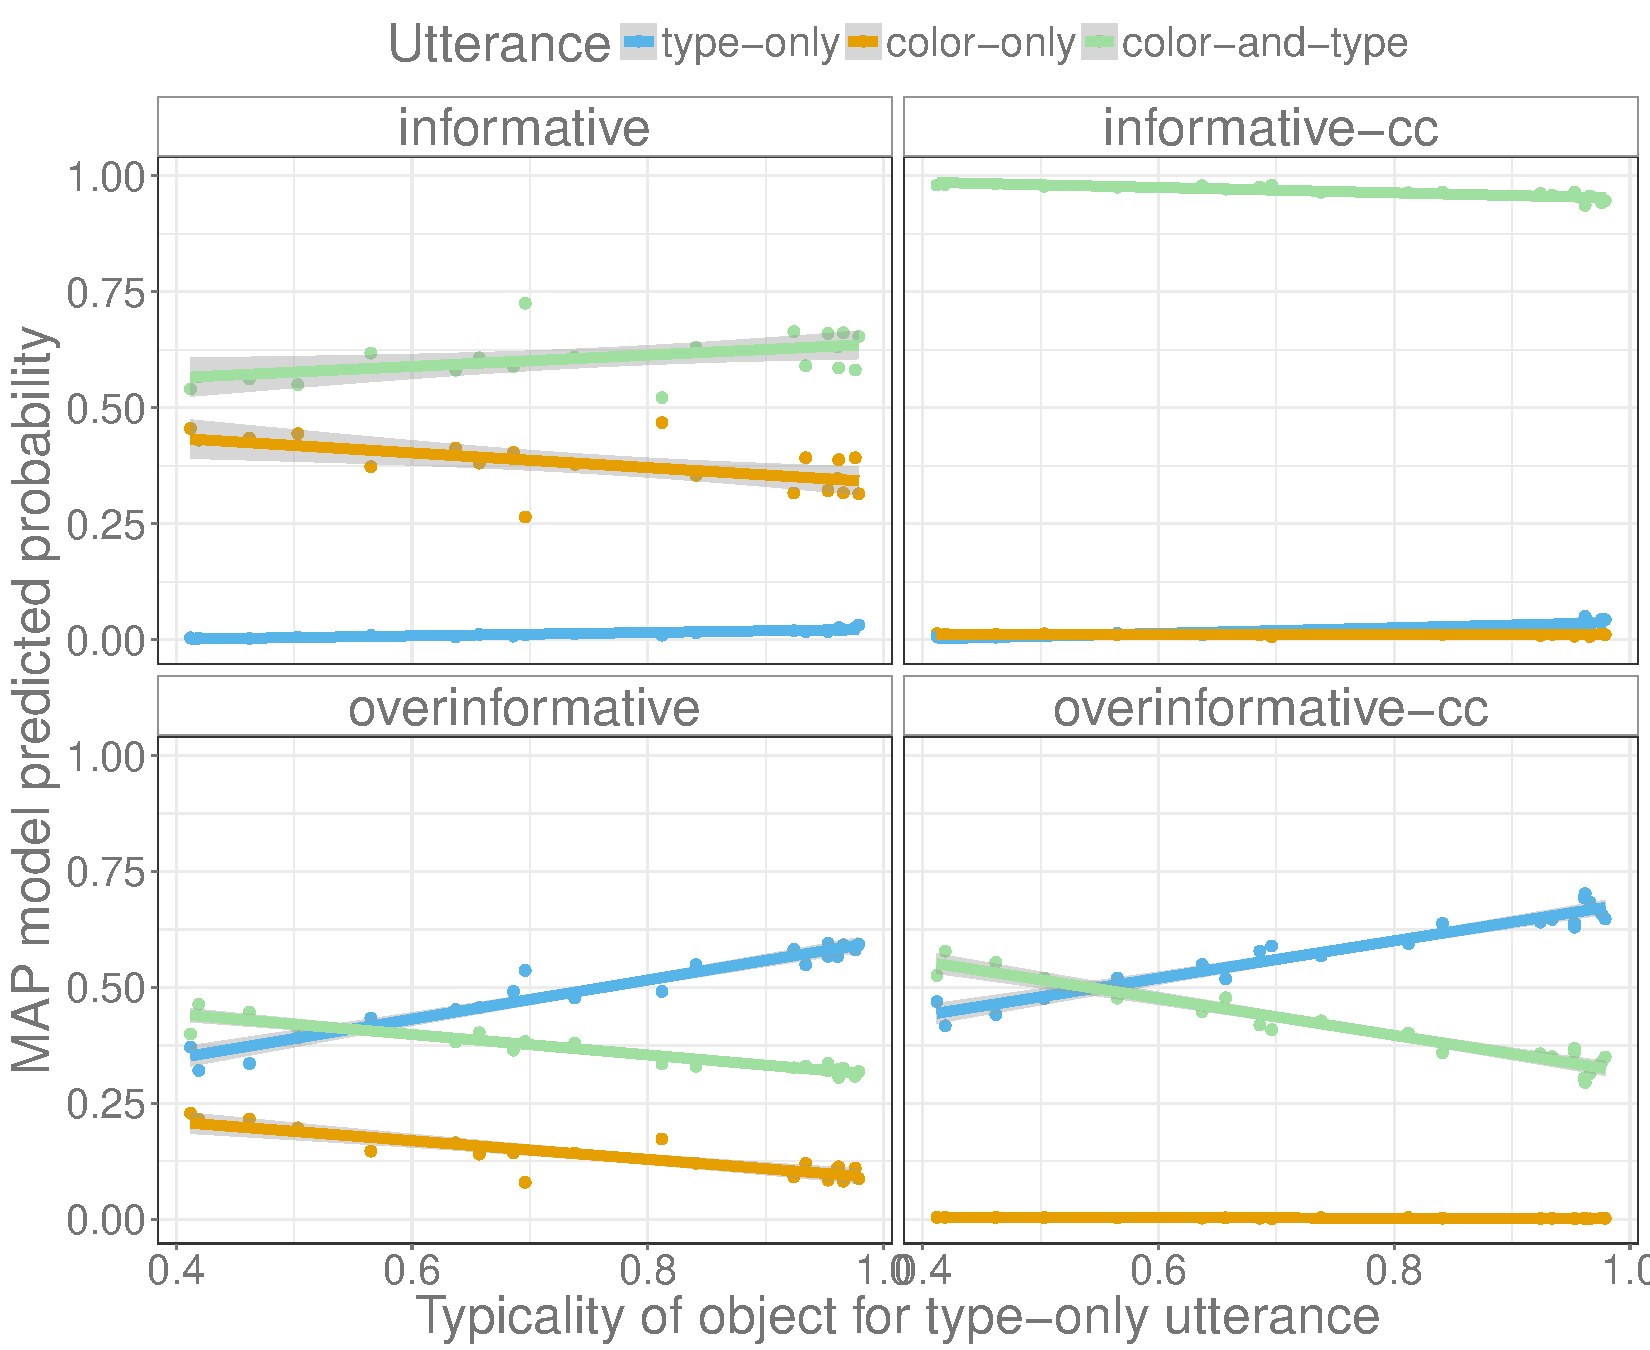
\includegraphics[width=.77\textwidth]{pics/exp2-none-fixedplusempirical-predictives}
		\caption{MAP model predicted utterance probabilities}
		\label{fig:exp2model}
	\end{subfigure}
%\caption{MAP model predicted utterance probabilities for each target as a function of mean object typicality for the type-only utterance (e.g., \emph{banana}). Color indicates utterance type: color-only (\emph{yellow}), type-only (\emph{banana}), color-and-type (\emph{yellow banana}). Facets indicate conditions.}
\caption{(a) Empirical utterance proportions in Exp.~2 and (b) MAP model predicted utterance probabilities for each target as a function of mean object typicality for the type-only utterance (e.g., \emph{banana}). Color indicates utterance type: type-only (\emph{banana}), color-only (\emph{yellow}), color-and-type (\emph{yellow banana}), and other (\emph{funky carrot}). Facets indicate conditions. Modified utterance data points for the banana items are circled in the banana's respective color in (a).}
\label{fig:exp2results}
\end{figure}




The following questions are of interest. First, do we replicate the previously documented typicality effect on redundant color mention (as suggested by the visual inspection of the banana item)? Second, does typicality affect color mention even when color is informative (i.e., technically necessary for establishing unique reference)? Third, are speakers sensitive to the presence of color competitors in their use of color or are typicality effects immune to the nature of the distractor items?

To address these questions we conducted a mixed effects logistic regression predicting color use from fixed effects of typicality, informativeness, and color competitor presence. We used the typicality norms obtained in the \emph{type}/object typicality elicitation study reported above (see \figref{fig:obj}) as the continuous typicality predictor. The informativeness condition was coded as a binary variable (color informative vs.~color overinformative trial) as was color competitor presence (absent vs.~present). All predictors were centered before entering the analysis. The model included by-speaker and by-item random intercepts, which was the maximal random effects structure that allowed the model to converge.

There was a main effect of typicality, such that the more typical an object was for the type-only utterance, the lower the log odds of color mention ($\beta$ = -4.17, $SE$ = 0.45, $p <$ .0001), replicating previously documented typicality effects. Stepwise model comparison revealed that including interaction terms was not justified by the data, suggesting that speakers produce more typical colors less often even when the color is in principle necessary for establishing reference (i.e., in the informative conditions). This is notable: speakers sometimes call a yellow banana simply a \emph{banana} even when other bananas are present, presumably because they can rely on listeners drawing the inference that they must have meant the most typical banana. In contrast, blue bananas' color is always mentioned in the informative conditions.

There was also a main effect of informativeness, such that color mention was less likely when it was overinformative than when it was informative ($\beta$ = -5.56, $SE$ = 0.33, $p <$ .0001). Finally, there was a main effect of color competitor presence, such that color mention was more likely when a color competitor was absent  ($\beta$ = 0.71, $SE$ = 0.16, $p <$ .0001). This suggests that speakers are indeed sensitive to the contextual utility of color -- color typicality alone does not capture the full set of facts about color mention, as we already saw in \sectionref{sec:rsaevaluationbasicscene}.


\subsection{Model evaluation}
\label{sec:colorypicalitymodel}


We evaluated the continuous semantics RSA model on the obtained production data from Exp.~2. In particular, we were interested in using model comparison to address the following issues. 

First, we already discussed that at least for the banana item, the empirically elicited typicalities, when interpreted as semantic values, capture qualitative  patterns in the data that the simple modifier type noise asymmetry assumed in the previous section cannot capture. Is this more fine-grained treatment of semantic values as capturing an object's typicality as an instance of an utterance enough to account for speakers' choice of expression, or is it necessary to integrate both the empirically elicited values and the utterance type level (color, type) noise values?

Second, we can ask whether or not utterance cost, quantified in two different ways, explains any of the observed production behavior. 

While the architecture of the model remained the same as that of the model presented in \sectionref{sec:modifiedmodel}, we briefly review the minor necessary changes, some of which we already mentioned at the beginning of this section. These changes concerned the lexicon and the cost function.\footnote{See \tableref{tab:modeldiffs} for an overview of the models reported in the paper.} We elaborate on each in turn before turning to the model evaluation. 

\subsubsection{Lexicon}

Whereas for the purpose of evaluating the model in \sectionref{sec:rsaevaluationbasicscene}  we only considered the utterance alternatives \emph{color}, \emph{size}, and \emph{color-size}, collapsing over the precise level of attributes, here we included in the lexicon each possible color adjective, type noun, and combination of the two. This substantially increased the size of the lexicon to 37 unique utterances. For each combination of utterance $u$ and object $o$ that occurred in the experiment, we included a separate semantic value $x_{u,o}$, elicited in the norming experiments described in \sectionref{sec:typicalitynormingcolor} (rather than inferred as done for Exp.~1, to avoid overfitting).\footnote{Ideally, one would like to derive the semantic values for the modified utterances from the semantic values of the individual lexical items.  Unfortunately, the compositionality of continuous values is a recognized problem \cite{kamp1995} and not one we aim to solve here. For our purposes it was therefore sufficient that we had access to the semantic values of the modified utterances elicited experimentally.} For any given context, we assumed the utterance alternatives that correspond to the individually present features and their combinations. For example, for the context in \figref{fig:condOverinfcc}, the set of utterance alternatives was \emph{yellow, green, pear, banana, avocado, yellow pear, yellow banana}, and \emph{green avocado}. 

\subsubsection{Semantics}

We compared two choices of semantics for the model.
In the \emph{empirical semantics} version, the empirically elicited typicality values were directly used as semantic values.
In the more complex \emph{fixed plus empirical semantics} version, we introduce an additional parameter interpolating between the empirical typicality values and inferred values for each utterance type as  employed in \sectionref{sec:rsaevaluationbasicscene} (e.g. one value for color terms and another for type terms, which are multiplied when the terms are composed in an utterance).
Note that this allows us to perform a nested model comparison, since the first model is a special case of the second.
%by comparing the \emph{empirical semantics} model to a  model that combined empirical typicality values and fixed expression type level noise terms in the following way:

\subsubsection{Cost function}

For the purpose of evaluating the model in \sectionref{sec:rsaevaluationbasicscene} we inferred two constant costs (one for color and one for size), and found in the Bayesian Data Analysis that the role of cost in explaining the data was minimal at best. Here, we compared two different versions of utterance cost. In the \emph{fixed cost} model we treated cost the same way as in the previous section and included only a color and type level cost, inferred from the data. We then compared this model to an \emph{empirical cost model}, in which we included a more complex cost function. 
Specifically, we defined utterance cost $c(u)$ as follows:
\begin{equation} \label{eq:exp2cost}
c(u) = \beta_F\cdot p(u) + (1-\beta_F)\cdot l(u)
\end{equation}

Here, $p(u)$ is utterance frequency as estimated from the Google Books corpus (years 1950 to 2008); $l(u)$ is the mean empirical length of the utterance in characters in the production data (e.g., sometimes \emph{yellow} was abbreviated as \emph{yel}, leading to an $l(u)$ smaller than 6); and $\beta_F$ is a weight that interpolates between length and frequency (when 1, cost is only a function of frequency; when 0, cost is only a function of length). Both $p(u)$ and $l(u)$ were normalized to fall into the interval $[0,1]$. The empirical cost function thus prefers short and frequent utterances (e.g., \emph{blue}) over long and infrequent ones (\emph{turquoise-ish bananaesque thing}).
We compared both of these models to a simpler baseline in which utterances were assumed to have no cost.

\subsubsection{Model comparison}

To evaluate the effect of these choices of semantics and cost, we conducted a full Bayesian model comparison.
Specifically, we compute the Bayes Factor for each comparison, a measure quantifying the support for one model over another in terms of the relative likelihood they each assign to the data.
As opposed to classical likelihood ratios, which only use the maximum likelihood estimate, the likelihoods in the Bayes Factor integrate over all parameters, thus automatically applying an Occam's Razor correcting for over-fitting. 
Because it was intractable to analytically compute these integrals for our recursive model, we used Annealed Importance Sampling (AIS), a Monte Carlo algorithm commonly used to approximate these quantities.
To ensure high-quality estimates, we took the mean over 100 independent samples for each model, with each chain running for 30,000 steps.
The marginal log likelihoods for each model are shown in \tableref{tab:exp2-modelcomparison}. 
The best performing model used \emph{fixed plus empirical} semantics and did not include a cost term. 
Despite the greater number of parameters associated with adding the fixed semantics to the empirical semantics, the \emph{fixed plus empirical} semantics models were preferred across the board compared to their empirical-only counterparts ($BF = 3.7 \times 10^{48}$ for fixed costs, $BF = 2.1 \times 10^{60}$ for empirical costs, and $BF = 1.4 \times 10^{71}$ for no cost). 
In comparison, additional cost-related parameters were not justified, with $BF = 5.7 \times 10^{21}$ for no cost compared to fixed cost and $BF = 2.1 \times 10^{27}$ for compared to empirical cost.

\begin{table}
\caption{Marginal log likelihood for each model. Best model is in bold. Parentheses indicate number of free parameters.}
\centering
\begin{tabular}{l l c c }
\toprule
& & \multicolumn{2}{c}{Semantics}\\
& & \emph{empirical} & \emph{fixed plus empirical}\\
\midrule
\multirow{3}{*}{Cost} & \emph{empirical} & -1474.6 (4) & -1354.4 (7) \\
 & \emph{fixed} & -1434.8 (4) & -1321.9 (7) \\
 & \emph{none} & -1372.9 (2) & \textbf{-1209.8 (5)} \\ 
\bottomrule
\end{tabular}
\label{tab:exp2-modelcomparison}
\end{table}

The correlation between empirical utterance proportions and the best model's MAP predictions at the by-item level was $r=.94$. Predictions for the best-performing model are visualized alongside empirical proportions in \figref{fig:exp2model}. The model successfully reproduces the empirically observed typicality effects in all four experimental conditions. However, we note that it diverges somewhat from the empirical data in conditions without color competitors. Here, \emph{color-and-type} utterances are systematically somewhat underpredicted in the informative condition, and systematically somewhat overpredicted in the overinformative condition. The reverse is true for \emph{color-only} utterances. It is worth looking at the posterior over parameters, shown in \figref{fig:typparamposteriors}, to understand the pattern. In particular, the utterance type level semantic value of type is inferred to be systematically higher than that of color, capturing that type utterances are less noisy than color utterances.\footnote{Interestingly, the inferred semantic value for color is very similar in absolute terms to that in Exp.~1.} An increase in \emph{color-only} mentions in the overinformative condition could be achieved by reducing the semantic value for type. However, that would lead to a further increase in \emph{color-only} mentions in the informative condition as well. That is, the two conditions are in a tug-of-war with each other.

\begin{figure}
\centering
%\includegraphics[width=\textwidth]{../../../models/1a_bda_basic/results_bda/graphs/parameterposteriors-fixed-reducedconditions}
% old location \includegraphics[width=\textwidth]{../../../models/old/1a_bda_basic/results_bda/graphs/parameterposteriors-fixed-reducedconditions-unlogged}
%\includegraphics[width=\textwidth]{pics/parameterposteriors-fixed-reducedconditions-unlogged}
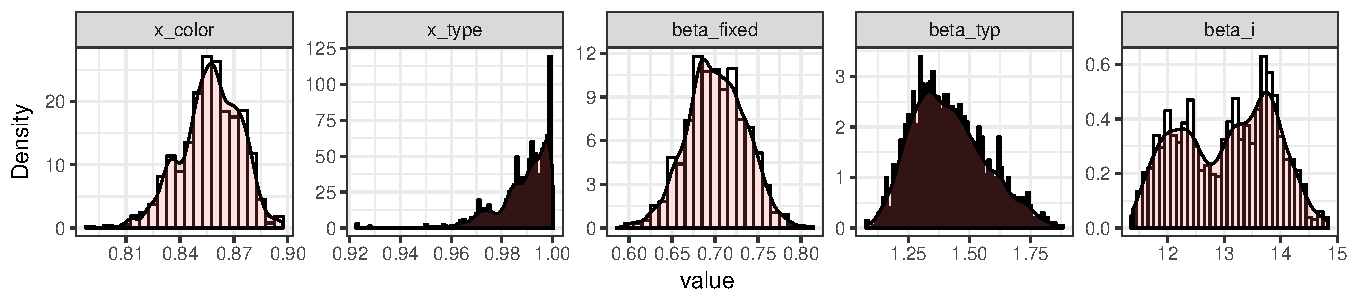
\includegraphics[width=\textwidth]{pics/exp2-cost-none-sem-fixedplusempirical-paramposteriors}
\caption{For best model, posterior model parameter distributions for utterance type level semantic values (color, type), interpolation weight on fixed vs.~empirical semantics, typicality stretching parameter, and weight on informativity. Maximum a posteriori (MAP)  $x_{\textrm{color}}$ = 0.86, 95\% highest density interval (HDI) = [0.82,0.89]; MAP $x_{\textrm{type}}$ = 0.998, HDI = [0.97,1.00]; $\beta_{\textrm{fixed}}$ = .69, HDI = [0.64, 0.77]; MAP $\beta_{\textrm{typ}}$ = 1.34, HDI = [1.19,1.75]; MAP $\beta_i$ = 13.74, HDI = [11.58,14.37].}
\label{fig:typparamposteriors}
\end{figure}

Two further things of note: the interpolation weight between the fixed and empirical semantic values is in the intermediate range: this provides evidence that a noisy truth-conditional semantics as employed in Exp.~1 is justified, but that taking into account graded category membership or typicality in an utterance's final semantic value is also necessary. That the weight on the empirically elicited typicalities is slightly higher than 1 suggests that the empirically elicited typicalities were somewhat less extreme than represented underlyingly.



\subsection{Discussion}

In this section we demonstrated that the continuous semantics RSA model predicts color typicality effects in the production of referring expressions. The model employed here did not differ in its architecture from that employed in \sectionref{sec:rsaevaluationbasicscene}, but only in that a) semantic values were assumed to operate at the individual utterance/object level in addition to at the utterance type/object level; b) semantic values were empirically elicited via typicality norming studies in addition to being inferred from the data; and c) an utterance's cost was assumed to be a function of its mean empirical length and its corpus frequency as estimated from a large corpus instead of having a constant utterance type level value, though utterance cost ultimately was found not to play a role in predicting utterance choice.\footnote{See \tableref{tab:modeldiffs} for a more extensive overview of the ways in which the models reported across sections differed.} 

This suggests that the dynamics at work in the choice of color vs.~size and in the choice of color as a function of the object's color typicality are very similar: speakers choose utterances by considering the fine-grained differences in information about the intended referent communicated by the ultimately chosen utterance compared to its competitor utterances. For noisier utterances (e.g., \emph{banana} as applied to a blue banana), including the `overinformative' color modifier is useful because it provides information. For less noisy utterances (e.g., \emph{banana} as applied to a yellow banana), including the color modifier is useless because the unmodified utterance is already highly informative with respect to the speaker's intention. These dynamics can sometimes even result in the color modifier being left out altogether, even when there is another object of the same type present that is very atypical, simply because the literal listener asymmetry in probability of choosing the intended referent over the competitor object is big enough.

Crucially, model comparison demonstrated the need for assuming a semantics that interpolates between a noisy truth-conditional semantics as employed in Exp.~1 and empirically elicited semantic values. This suggests that speakers, in choosing utterances, take into account both an utterance's literal semantics and its noisiness, as well as the graded category membership of the objects under consideration. Perhaps surprisingly, we replicated the result from Exp.~1 that utterance cost does not add any predictive power, even when quantified via a more sophisticated cost function that takes into account an utterance's length and frequency.

In the next section, we move beyond the choice of modifier and ask whether continuous semantics RSA provides a good account of content selection in referring expressions more generally. To answer this question we turn to simple nominal referring expressions.

\section{Unmodified referring expressions: nominal taxonomic level}
\label{sec:nominal}

In this section we investigate whether continuous semantics RSA accounts for referring expression production beyond the choice of modifier. In particular, we focus on speakers' choice of taxonomic level of reference in nominal referring expressions. A particular object can be referred to at its subordinate (\emph{dalmatian}), basic (\emph{dog}), or superordinate (\emph{animal}) level, among other choices. As discussed in \sectionref{sec:nominalintro},  multiple factors play a role in the choice of nominal referring expression, including an expression's contextual informativeness, its cognitive cost \cite<short and frequent terms are preferred over long and infrequent ones,>{griffin1998,jescheniak1994}, and its typicality \cite<an utterance is more likely to be used if the object is a good instance of it,> {Jolicoeur1984}.

Choice of taxonomic level (e.g., between \emph{dog} and \emph{dalmatian}) is analogous to the choice of modified referring expressions (e.g., between \emph{dog} and \emph{big dog}) in that the two expressions differ in how much information about the intended referent is provided. However, cost-wise, in contrast to the modifier case, the choice between different levels of reference does not result in a choice between a shorter or longer utterance in terms of the number of words required, but it is possible that differences in length and frequency of the different nouns affect the choice. Thus, effects of the same factors we previously tested for in the choice of modifier in the previous two sections can also be tested for their involvement in nominal choice.

In order to evaluate continuous semantics RSA for nominal choice, we proceeded as in \sectionref{sec:colortypicality}: we collected production data within the same reference game setting, but varied the contextual informativeness of utterances by varying whether distractors shared the same basic or superordinate category with the target (see \figref{fig:dogcontexts}). We also elicited typicality ratings for object-utterance combinations, which entered the model as the semantic values via the lexicon. We then conducted the same type of Bayesian data analysis as reported in the previous sections for model comparison.


\subsection{Experiment 3: taxonomic level of reference in nominal referring expressions}
\label{sec:exp3}

\subsubsection{Method}

\paragraph{Participants}

We recruited 58 pairs of participants (116 participants total, the same participants as in Exp.~1) over Amazon's Mechanical Turk who were each paid \$1.75 for their participation. 

\paragraph{Procedure and materials}

The procedure was identical to that of Exp.~1.\footnote{Exp.~3 constitutes a replication of the production experiment reported in \citeA{GrafEtAl2016}.} Participants proceeded through 72 trials. Of these, half were critical trials of interest and half were filler trials (the critical trials from Exp.~1). On critical trials, we varied the level of reference that was sufficient to mention for uniquely establishing reference.

Stimuli were selected from nine distinct domains, each corresponding to distinct basic level categories such as \emph{dog}.  For each domain, we selected four subcategories to form our target set (e.g. \emph{dalmatian}, \emph{pug}, \emph{German Shepherd} and \emph{husky}). See \tableref{tab:reflevelstimuli} in \appref{app:taxonomicstimuli} for a full list of domains and their associated target items. Each domain also contained an additional item which belonged to the same basic level category as the target (e.g., \emph{greyhound}) and items which belonged to the same supercategory but not the same basic level (e.g., \emph{elephant} or \emph{squirrel}). The latter items were used as distractors.


Each trial consisted of a display of three images, one of which was designated as the target object. Each pair of participants saw each target exactly once, for a total of 36 trials per pair. These target items were randomly assigned distractor items which were selected from three different context conditions, corresponding to different communicative pressures (see \figref{fig:dogcontexts}). The \emph{subordinate necessary} contexts contained one distractor of the same basic category and one distractor of the same superordinate category (e.g., target: \emph{dalmatian}, distractors: \emph{greyhound} (also a dog) and \emph{squirrel} (also an animal)). The \emph{basic sufficient} contexts contained either two distractors of the same superordinate category but different basic category as the target (e.g., target: \emph{husky}, distractors: \emph{hamster} and \emph{elephant}) or one distractor of the same superordinate category and one unrelated item (e.g., target: \emph{pug}, distractors: \emph{cow} and \emph{table}). The \emph{superordinate sufficient} contexts contained two unrelated items (e.g., target: \emph{German Shepherd}, distractors: \emph{shirt} and \emph{cookie}). 

\begin{figure}
	\begin{subfigure}{.5\textwidth}
		\centering
		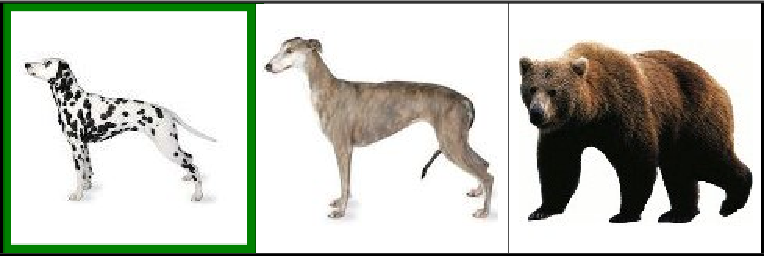
\includegraphics[width=.8\textwidth]{pics/item12.pdf}
		\caption{subordinate necessary}
		\label{fig:item12}
	\end{subfigure}
	\begin{subfigure}{.5\textwidth}
		\centering
		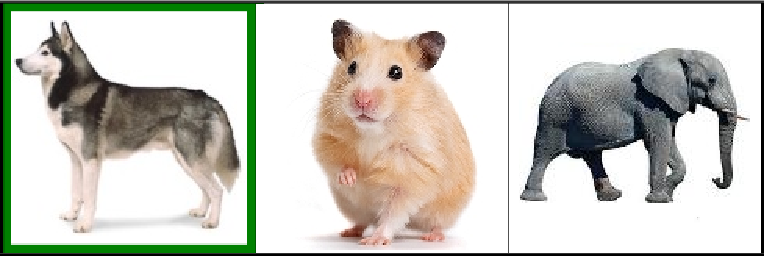
\includegraphics[width=.8\textwidth]{pics/item22.pdf}
		\centering
		\caption{basic sufficient (two superordinate distractors)}
		\label{fig:item22}
	\end{subfigure}
	\begin{subfigure}{.5\textwidth}
		\centering
		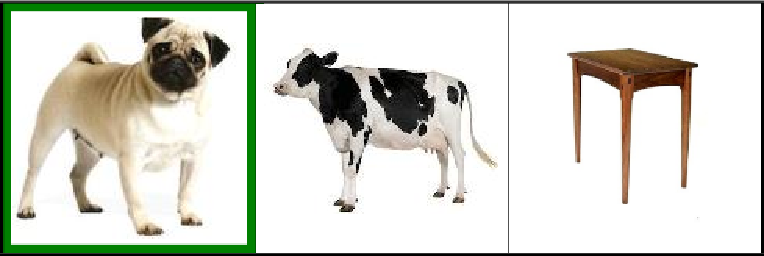
\includegraphics[width=.8\textwidth]{pics/item23.pdf}
		\caption{basic sufficient (one superordinate distractor)}
		\label{fig:item23}
	\end{subfigure}
	\begin{subfigure}{.5\textwidth}
		\centering
		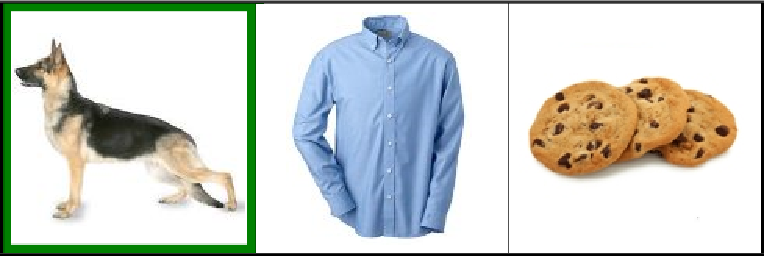
\includegraphics[width=.8\textwidth]{pics/item33.pdf}
		\centering
		\caption{superordinate sufficient}
		\label{fig:item33}
	\end{subfigure}
	\caption{Example contexts in which different levels of reference are necessary for establishing unique reference to the target marked with a green border: (a) subordinate necessary (\emph{dalmatian}); (b, c) basic sufficient (\emph{dog}) and subordinate possible (\emph{husky}, \emph{pug}); (d) superordinate sufficient (\emph{animal}) and basic or subordinate possible (\emph{dog}, \emph{German Shepherd}).}
	\label{fig:dogcontexts}
\end{figure}

This context manipulation served as a manipulation of utterance informativeness: any target could be referred to at the subordinate (\emph{dalmatian}), basic (\emph{dog}) or superordinate (\emph{animal}) level. However, the level of reference necessary for uniquely referring differed across contexts.


\subsubsection{Data pre-processing and exclusion}

We collected 2193 referring expressions. To determine the level of reference for each trial, we followed the following procedure. First, speakers' and listeners' messages were parsed automatically; the referring expression used by the speaker was extracted for each trial and checked for whether it contained the current target's correct \emph{sub}(ordinate), \emph{basic}, or \emph{super}(ordinate) level term using a simple grep search. In this way, 71.4\% of trials were labelled as mentioning a pre-coded level of reference. In the next step, remaining utterances were checked manually by one of the authors (CG) to determine whether they contained a correct level of reference term which was not detected by the grep search due to typos or grammatical modification of the expression. In this way, meaning-equivalent alternatives such as \emph{doggie} for \emph{dog}, or reduced forms such as \emph{gummi}, \emph{gummies} and \emph{bears} for \emph{gummy bears} were counted as containing the corresponding level of reference term. This covered another 15.0\% of trials. 41 trials on which the listener selected the wrong referent were excluded, leading to the elimination of 2.1\% of trials. Six trials were excluded because the speaker did not produce any utterances. Additionally, a total of 12.5\% of correct trials were excluded because the utterance consisted only of an attribute of the superclass (\emph{the living thing} for \emph{animal}), of the basic level (\emph{can fly} for \emph{bird}), of the subcategory (\emph{barks} for \emph{dog}) or of the particular instance (\emph{the thing facing left}) rather than a category noun. These kinds of attributes were also mentioned in addition to the noun on trials which were included in the analysis for 8.9\% of sub level terms, 18.9\% of basic level terms, and 60.9\% of super level terms. On 1.2\% of trials two different levels of reference were mentioned; in this case the more specific level of reference was counted as being mentioned in this trial. After all exclusion and pre-processing, 1872 cases classified as one of \emph{sub}, \emph{basic}, or \emph{super} entered into the analysis.


\subsubsection{Results and discussion}


Proportions of sub, basic, and super level utterances are shown in \figref{fig:exp2results}. Overall, super level mentions are highly dispreferred ($< 2\%$), so we focus in this section only on predictors of sub over basic level mentions. The clearest pattern of note is that sub level mentions are only preferred in the most constrained context that necessitates the sub level mention for unique reference (e.g., target: dalmatian, distractor: greyhound; see \figref{fig:item12}). Nevertheless, even in these contexts there is a non-negligible proportion of basic level mentions (28\%).\footnote{This context is analogous to the informative contexts from Exp.~2, where we also observed some `underinformative' referring expressions, but note that here this proportion is even higher.} In the remaining contexts, where the sub and basic level are equally informative, there is a clear preference for the basic level. In addition, mitigating this context effect, sub level mentions increased with increasing typicality of the object as an instance of the sub level utterance.


\begin{figure}
\centering
%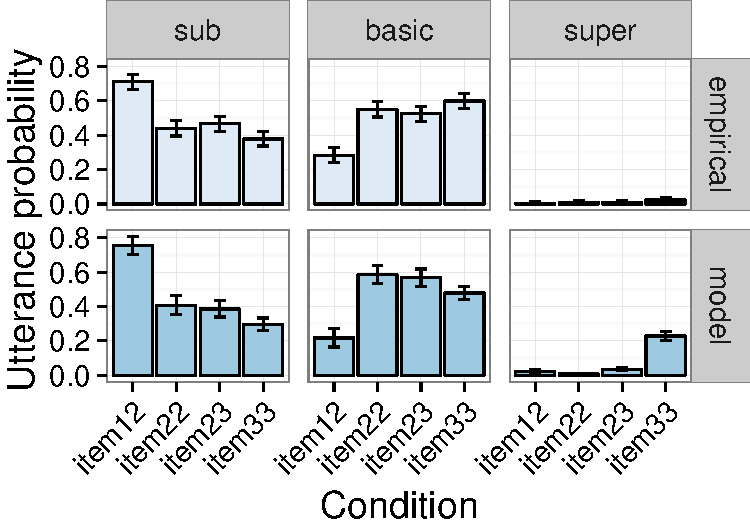
\includegraphics[width=.7\textwidth]{pics/qualitativepattern-fulldataset-typicalities-hmc}
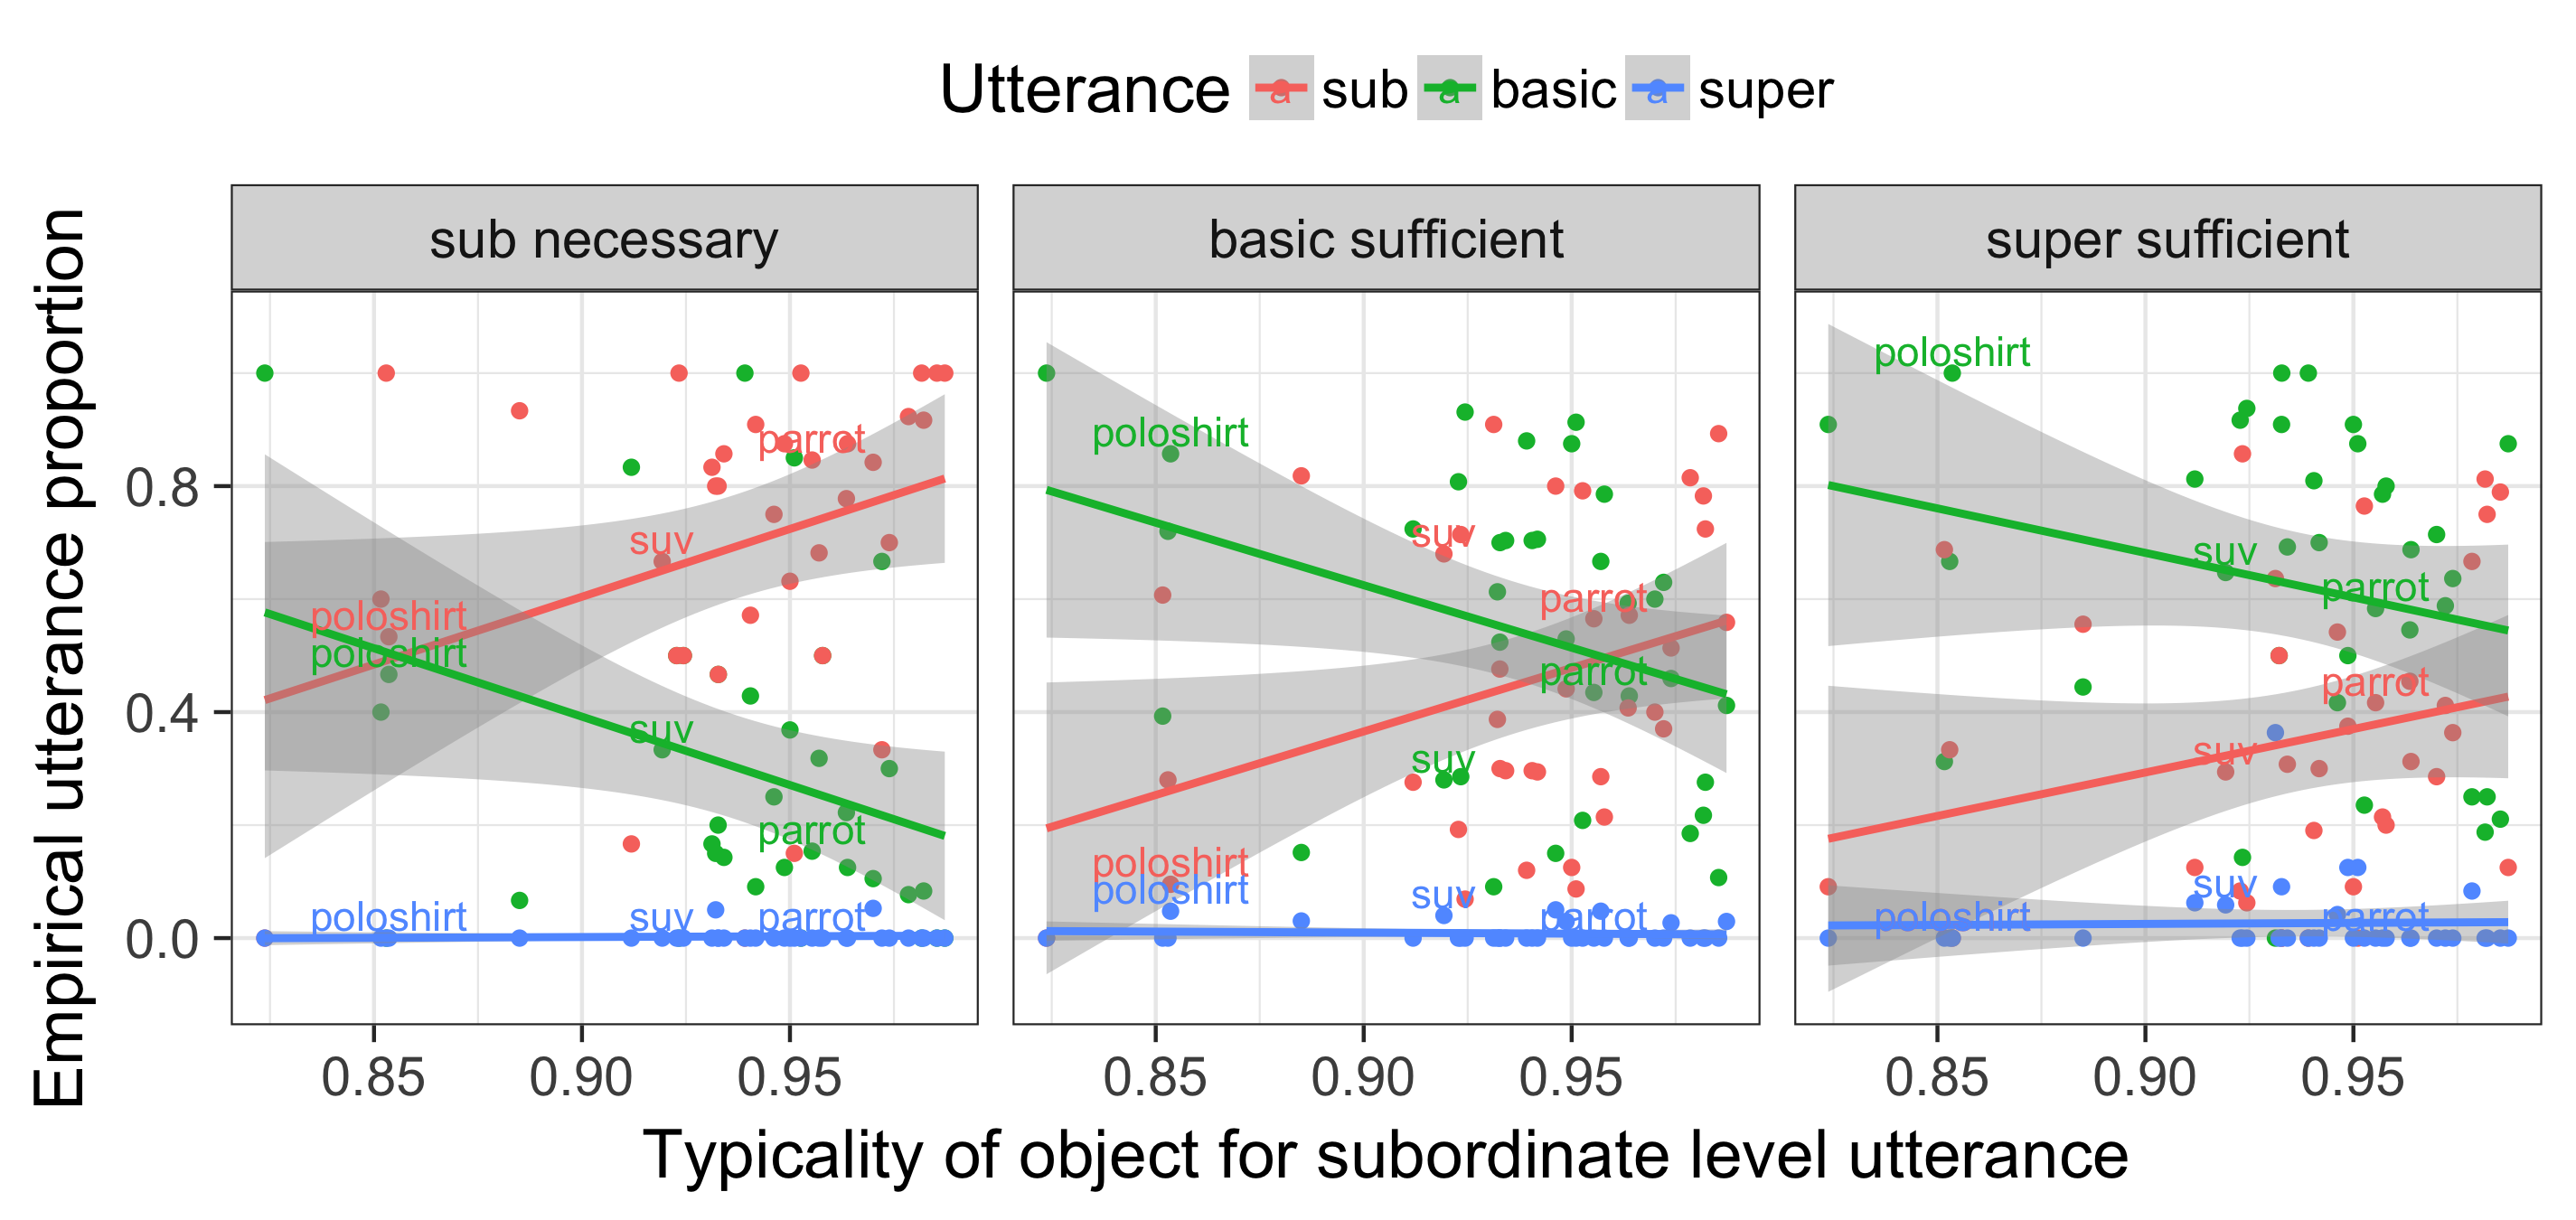
\includegraphics[width=.9\textwidth]{pics/results-exp3.png}
\caption{Utterance proportions for each target item across different informativeness conditions as a function of the object's subordinate level typicality. Example target items \emph{polo shirt} (basic: \emph{shirt}, super: \emph{clothes}),  \emph{SUV} (basic: \emph{car}, super: \emph{vehicle}), and \emph{parrot} (basic: \emph{bird}, super: \emph{animal}) that were characteristic of relatively low to relatively high sub typicality items are labeled explicitly.}
\label{fig:exp2results}
\end{figure}

What explains these preferences? In order to test for effects of informativeness, length, frequency, and typicality on nominal choice we conducted a mixed effects logistic regression predicting sub over basic level mention from centered predictors for the factors of interest and the maximal random effects structure that allowed the model to converge (random by-speaker and by-target intercepts).\footnote{In order to address convergence issues with \verb+lmer+ when specifying the full random effects structure -- i.e., by-speaker and by-item random intercepts and slopes for all fixed effects -- we also ran a Bayesian binomial mixed effects model with weakly informative priors using the \verb+brms+ package \cite{brms} that included the same fixed effects structure as the lmer model and the full random effects structure. The results were qualitatively identical, yielding  evidence for main effects of context (sub vs basic sufficient: posterior mean $\beta$ = 2.44, $95\%$ CI = $[$1.87,3.06$]$, $p(\beta > 0)$ = 1; basic vs super sufficient: posterior mean $\beta$ = 0.70, $95\%$ CI = $[$0.32,1.09$]$, $p(\beta > 0)$ = 1), typicality (posterior mean $\beta$ = 9.96, $95\%$ CI = $[$3.55,17.51$]$, $p(\beta > 0)$ = 1), and length (posterior mean $\beta$ = -1.12, $95\%$ CI = $[$-2.00,-0.31$]$, $p(\beta < 0)$ = 1).} 

\emph{Frequency} was coded as the difference between the sub and the basic level's log frequency, as extracted from the Google Books Ngram English corpus ranging from 1960 to 2008. 

\emph{Length} was coded as the ratio of the sub to the basic level's length. We used the mean empirical lengths in characters of the utterances participants produced. For example, the minivan, when referred to at the subcategory level, was sometimes called ``minivan'' and sometimes ``van'' leading to a mean empirical length of 5.71. This is the value that was used, rather than 7, the length of ``minivan''. That is, a higher frequency difference indicates a \emph{lower} cost for the sub level term compared to the basic level, while a higher length ratio reflects a \emph{higher} cost for the sub level term compared to the basic level.\footnote{We replicate the well-documented negative correlation between length and log frequency ($r = -.49$ in our dataset).} 

\emph{Typicality} was coded as the ratio of the target's sub to basic level label typicality.\footnote{Typicalities were elicited in a separate norming study that was identical in procedure to that of Exp.~1a. See \appref{app:typicalitynorms2} for details about the study.} That is, the higher the ratio, the more typical the object was for the sub level label compared to the basic level; or in other words, a higher ratio indicates that the object was relatively atypical for the basic label compared to the sub label. For instance, the panda was relatively atypical for its basic level ``bear'' (mean rating 0.75) compared to the sub level term ``panda bear'' (mean rating 0.98), which resulted in a relatively \emph{high} typicality ratio.

\emph{Informativeness} condition was coded as a three-level factor: \emph{sub necessary}, \emph{basic sufficient}, and \emph{super sufficient}, where \emph{basic sufficient (two superordinate distractors)} and \emph{basic sufficient (one superordinate distractor)} were collapsed into \emph{basic sufficient}. Condition was Helmert-coded: two contrasts over the three condition levels were included in the model, comparing each level against the mean of the remaining levels (in order: \emph{sub necessary}, \emph{basic sufficient}, \emph{super sufficient}). This allowed us to determine whether the probabilities of type mention  for neighboring conditions were significantly different from each other, as suggested by \figref{fig:exp2results}.

%\begin{table}[!tbp]
%\begin{center}
%\begin{tabular}{lrrl}
%\toprule
%\multicolumn{1}{l}{}&\multicolumn{1}{c}{Coef $\beta$}&\multicolumn{1}{c}{SE($\beta$)}&\multicolumn{1}{c}{$p$}\tabularnewline
%\midrule
%Intercept&$-0.02$&$0.27$&\textgreater 0.93\tabularnewline
%Condition sub.vs.rest&$ 2.05$&$0.17$&\textbf{\textless .0001}\tabularnewline
%Condition basic.vs.super&$ 0.54$&$0.15$&\textbf{\textless .001}\tabularnewline
%Frequency&$ 0.07$&$0.10$&\textgreater 0.5\tabularnewline
%Length&$-0.95$&$0.27$&\textbf{\textless .001}\tabularnewline
%Typicality&$ 4.84$&$1.32$&\textbf{\textless .001}\tabularnewline
%\bottomrule
%\end{tabular}\end{center}
%
%\end{table}

The log odds of mentioning the sub level term were greater in the \emph{sub necessary} condition than in either of the other two conditions ($\beta = 2.11$, $SE = .17$, $p < .0001$), and greater in the \emph{basic sufficient} condition than in the \emph{super sufficient} condition ($\beta = .60$, $SE = .15$, $p < .0001$), suggesting that the contextual informativeness of the sub level mention has a gradient effect on utterance choice.\footnote{Importantly, model comparison between the reported model and one that subsumes basic and super under the same factor level revealed that the three-level condition variable is justified ($\chi ^2 (1) = 12.82$, $p < .0004$), suggesting that participants don't simply revert to the basic level unless contextually forced not to.} There was also a main effect of typicality, such that the sub level term was preferred for objects that were more typical for the sub level compared to the basic level  description ($\beta = 4.82$, $SE = 1.35$, $p < .001$). In addition, there was a main effect of length, such that as the length of the sub level term increased compared to the basic level term (``chihuahua''/``dog'' vs.~``pug''/``dog''), the sub level term was dispreferred (``chihuahua'' is dispreferred compared to ``pug'', $\beta = -.95$, $SE = .27$, $p < .001$). The main effect of frequency did not reach significance ($\beta = .08$, $SE = .11$, $p < .45$).


%
%\begin{figure}
%\centering
%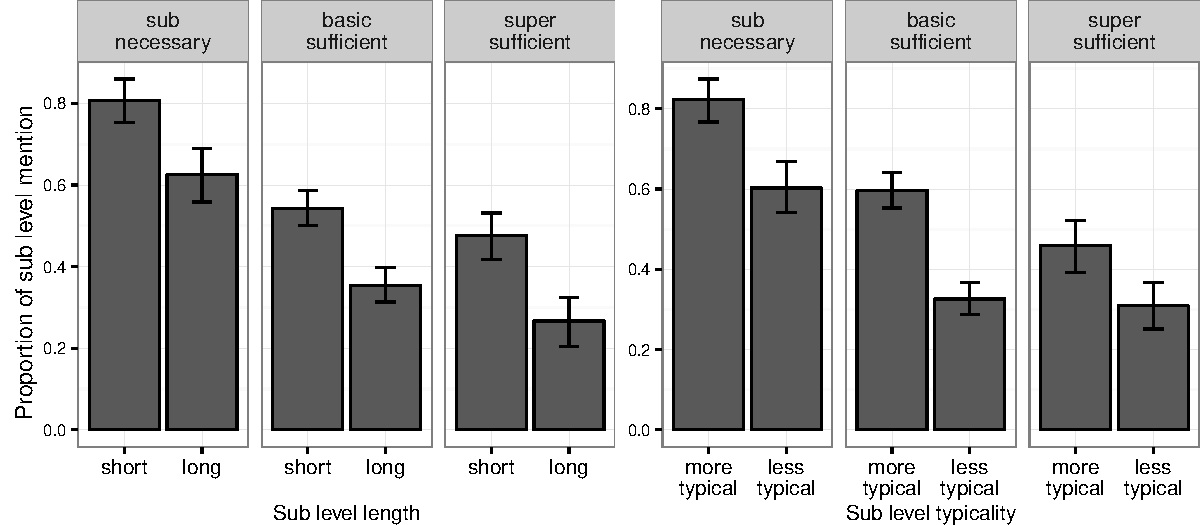
\includegraphics[width=\textwidth]{pics/lengthtypicality}
%\caption{Proportion of sub level (over sub and basic level) mentions across conditions. Left: when the sub  length is relatively short (.67,1.82] or long [1.82,4.3) compared to the basic level term. Right: when the target object was relatively more [1.06,1.91) or less (.88,1.06] typical for the sub compared to the basic level term. Length and typicality ratio intervals were generated by splitting data into groups of roughly equal numbers of observations.\jd{get rid of these figures -- integrate the typicality result into the first results figure (analogous to exp 2), and just report length/frequency without visualizing}}
%\label{fig:exp2effects}
%\end{figure}


Unsurprisingly, there was also significant by-participant and by-domain variation in sub level term mention. %\figref{fig:bigscatterplot} shows the by-domain variation in utterance choice. 
For instance, mentioning the sub over the basic level term was preferred more in some domains (e.g. in the ``candy'' domain) than in others. Likewise, some domains had a greater preference for basic level terms (e.g. the ``shirt'' domain). Using the super term also ranged from hardly being observable (e.g., \emph{plant} in the ``flower'' domain) to being used more frequently (e.g., \emph{furniture} in the ``table'' domain and \emph{vehicle} in the ``car'' domain). 

We thus replicated the well-documented preference to refer to objects at the basic level, which is partly modulated by contextual informativeness and partly a result of the basic level term's cognitive cost and typicality compared to its sub level competitor, mirroring the results from Exp.~2. 

Perhaps surprisingly, we did not observe an effect of frequency on sub level term mention. This is likely due to the modality of the experiment: the current study was a written production study, while most studies that have identified frequency as a factor governing production choices are spoken production studies. It may be that the cognitive cost of typing longer words may be disproportionately higher than that of producing longer words in speech, thus obscuring a potential effect of frequency. Support for this hypothesis comes from studies comparing written and spoken language, which has found that spoken descriptions are likely to be longer than written descriptions and, in English, seem to have a lower propositional information density than written descriptions \cite{VanMiltenburg2018}.



\subsection{Model evaluation}
\label{sec:reflevelmodel}


We evaluated the continuous semantics RSA model on the obtained production data from Exp.~3. The architecture of the model is identical to that of the model presented in \sectionref{sec:colorypicalitymodel}. The only difference is that the set of alternatives contained only the three potential target utterances (i.e., the target's sub, basic, and super label).\footnote{See \tableref{tab:modeldiffs} for an overview of the models reported in the paper.} Whereas the modifier models from the previous sections treat all individual features and feature combinations represented in the display as utterance alternatives, the nominal choice model considers only the three different levels of reference to the target as alternatives, e.g., \emph{dalmatian}, \emph{dog}, \emph{animal}. That is, assuming a German Shepherd as a distractor, \emph{German Shepherd} is \emph{not} considered an alternative.

For the previous dataset, we tested which of three different semantics was most justified -- a fixed semantics with type-level semantic values, the empirically elicited semantics, or a combination of the two. For the current dataset, this question did not arise, because we investigated only one type of utterance -- nouns. We hence only considered the \emph{empirical} semantics. However, like in the previous dataset, we evaluated which cost function was best supported by the data: the one defined in \eqref{eq:exp2cost}, repeated here, or a simpler baseline in which utterances were assumed to have no cost: 

\begin{equation}
c(u) = \beta_F\cdot p(u) + (1-\beta_F)\cdot l(u)
\end{equation} 

We employed the same procedure as in the previous section to compute the Bayes Factor for the comparison between the two cost models, and to compute the posteriors over parameters  $\beta_i  \sim \mathcal{U}(0,20)$,  $\beta_{c(\textrm{freq})} \sim \mathcal{U}(0,5)$, $\beta_{c(\textrm{len})} \sim \mathcal{U}(0,5)$,, $\beta_t  \sim \mathcal{U}(0,5)$.

Posteriors over parameters are shown in \figref{fig:nomparamposteriors}. While an absolute comparison between the informativity and cost weights is not possible, it is worth noting that the weight on frequency is close to zero, i.e., in line with the results from the mixed effects regression, an utterance's length, but not its frequency, factors into the probabilitiy with which it is produced. The posterior on the typicality weight also suggests that the typicality values elicited empirically should be stretched somewhat to yield semantic values that are appropriate for computing informativity from.

\begin{figure}
\centering
\includegraphics[width=\textwidth]{pics/exp3-paramposteriors}
\caption{Posterior model parameter distributions for informativity weight ($\beta_i$), frequency cost weight  ($\beta_{c(\textrm{freq})}$), length cost weight ($\beta_{c(\textrm{len})}$), and typicality weight ($\beta_t $). Maximum a posteriori (MAP)  $\beta_i$ = 6.16, 95\% highest density interval (HDI) = [5.45,6.37]; MAP $\beta_{c(\textrm{freq})}$ = 0.69, HDI = [0.16,0.84]; MAP $\beta_{c(\textrm{len})}$ = 2.26, HDI = [1.95, 2.68]; MAP $\beta_t $ = 1.56, HDI = [1.43,1.77].}
\label{fig:nomparamposteriors}
\end{figure}

A scatterplot of empirical utterance proportions agains model predictions is shown in \figref{fig:nompredictives}. \jd{XXX discuss}


\begin{figure}
\centering
\includegraphics[width=\textwidth]{pics/exp3-empirical-predictives}
\caption{Scatterplot of empirical utterance proportions against model predictions.}
\label{fig:nompredictives}
\end{figure}





% DON'T NEED QUALITATIVE EXAMPLE?
%To understand the qualitative behavior of the model, we briefly delve into two aspects of the model: first, the effect of typicality on the literal listener (and, in consequence via the pressure to be informative) the speaker. And second, the effect of cost (utterance length and frequency) on the speaker.



% DON'T NEED TO EXPLAIN AGAIN?
%\subsubsection{Typicality effects}
%
%\paragraph{Literal listener behavior.} The literal listener's probability of choosing the target under different semantic values for the observed utterance are shown in \figref{fig:nominallistenertypicality}. In general: as the target's typicality as an instance of the utterance increases and the distractors' typicality decreases, the probability of the literal listener choosing the target increases. Subordinate level terms tend to fall in the upper right quadrant of this graph. Basic level terms in the \emph{sub necessary} conditions tend to fall in the lower right quadrant, while basic level terms in the \emph{basic sufficient} conditions tend to fall in the upper right quadrant as well.
%
%\begin{figure}
%\centering
%% old location: \includegraphics[width=.6\textwidth]{../../../models/old/6_qualitative_nom_L0/L0probs.png}
%\includegraphics[width=.6\textwidth]{pics/L0probs.png}
%\caption{Literal listener probability of choosing the target under different typicalities of the target (x-axis) or the distractors (y-axis for the observed utterance. For simplicity we assume equal typicality of both distractors. The remaining probability mass for each case is thus uniformly distributed over both distractors.\jd{say where sub/basic/super level terms tend to fall in heatmap once you've regenerated plot}}
%\label{fig:nominallistenertypicality}
%\end{figure}
%
%\paragraph{Pragmatic speaker behavior.} To understand the effect of typicality on the speaker's behavior it is useful to think about the problem of deciding which taxonomic level to refer at in terms of typicality gain, as we did in \sectionref{sec:colortypicality} for the choice between modified and unmodified expression. There, we found that relatively large target (compared to distractor) typicality gains in going from unmodified to modified expressions compared resulted in greater probability of overmodification. Here we observe the same effect in going from a higher (less specific) to a lower (more specific) taxonomic level. This can be seen in \figref{fig:nominalspeakertypicality}, which shows the probability of each utterance (sub, basic, or super) as a function of absolute target typicality as well as target typicality gain. Target typicality gain is the difference between the target's sub level typicality and the target's basic level typicality. Probabilities are shown for contexts with three items, always assuming $\alpha = 7$, but manipulating distractor typicality to simulate conditions analogous to our experimental conditions \emph{sub necessary}, \emph{basic sufficient}, and \emph{super sufficient}. Simulated distractor typicalities for sub, basic, and super level reference are shown in \tableref{tab:simulatedtyps}.
%
%\begin{figure}
%\centering
%% old location: \includegraphics[width=\textwidth]{../../../models/old/7_qualitative_nom_S1_typ/S1probs_typgainmap_alpha7.png}
%\includegraphics[width=\textwidth]{pics/S1probs_typgainmap_alpha7.png}
%\caption{Pragmatic speaker probability of choosing each utterance (sub, basic, super) under varying absolute target sub typicalities (x-axis) and target typicality gains (difference between sub and basic level term typicality, y-axis), assuming equal typicality values for both distractors. Rows indicate different simulated conditions.\jd{go back into script to see how you computed typicality gain here}}
%\label{fig:nominalspeakertypicality}
%\end{figure}
%
%\begin{table}
%\centering
%\caption{Overview of simulated distractor typicality (semantic) values for sub, basic, and super level utterances in simulated conditions. In contrast to the actual experimental conditions, we assume equal typicality values for both distractors.}
%\begin{tabular}{l l c c c}
%\toprule
%& & \multicolumn{3}{c}{Condition}\\
%& & sub necessary & basic sufficient & super sufficient\\
%\midrule
%\multirow{3}{*}{Utterance} & sub & 0 & 0 & 0 \\
%& basic & .8 & .1 & 0 \\
%& super & .8 & .8 & 0\\
%\bottomrule
%\end{tabular}
%\label{tab:simulatedtyps}
%\end{table}
%
%The blue areas in the graph indicate highest-probability regions. For example, as expected in the \emph{sub necessary} condition, the sub level term is the most likely one. However, in certain cases the basic level term also receives non-zero probability, notably when the target is a better instance of the basic than the sub level term, or (not pictured) when the typicality of the distractor as an instance of the basic level term is very low  (e.g., the typicality of the koala bear as an instance of "bear" was only 0.50). Indeed, the grizzly (with high typicality for basic level ``bear'', .97) is referred to as ``bear'' rather than ``grizzly bear'' in 85\% of \emph{sub necessary} conditions when the koala is the distractor. 
%
%In the \emph{basic sufficient} conditions, sub level reference is nevertheless strongly predicted when target sub typicality gain is positive (i.e., when the target is a much better instance of the sub than of the basic level term). An example of such a case is the panda bear, who received a sub level typicality of .98 and a basic level typicality of only .75. Indeed, even when basic level reference was sufficient, the panda was referred to as the ``panda'' 81\% of the time.
%
%These patterns mirror the typicality effects obtained via the mixed effects regression.


%\subsubsection{Cost effects}
%
%The additional effect of cost on nominal choice is straightforward: the costlier an utterance (relative to its alternatives), the less likely it is to be used. This pattern, too, is one observed in the mixed effects regression. For instance, the (short, less costly) pug is almost three times as likely as the (long, more costly) German Shepherd to be referred to by its subordinate level term in the \emph{basic sufficient} and \emph{super sufficient} conditions, where subordinate level reference is unnecessary. 
%
%\bigskip
%In \sectionref{sec:reflevelmodel} we showed that continuous semantics RSA captures the right kinds of qualitative effects as observed in the mixed effects regression. In the next section we evaluate how well the model captures nominal choice preferences quantitatively.




\jd{XXX -- thus far missing entirely. }

\begin{itemize}
	\item report correlations with empirical data at different levels: at individual item (u,o) level collapsing across distractors; maybe collapsing across 3 different typicality bins?
	\item discuss posteriors over params -- is alpha similar? is cost weight still low but with most weight on length? 
	\item potential comparison with different models:
	\begin{itemize}
		\item should we run a version that includes all the distractor labels as alternatives as well?
	\end{itemize}
\end{itemize}

% OLD PROSE

%\subsection{Model evaluation: nominal choice}
%\label{sec:reflevelmodeleval}
%
%In order to evaluate continuous semantics RSA for nominal choice, we repeated the same Bayesian data analysis as reported in \sectionref{sec:modifiermodeleval} and \sectionref{sec:modelevalcolortypicality} to generate model predictions and infer likely parameter values. We did so by conditioning on the observed production data (coded into \emph{sub}, \emph{basic}, and \emph{super} level mentions as described above) and integrating over the three free parameters $\alpha  \sim \mathcal{U}(0,20)$, $\beta_f  \sim \mathcal{U}(0,5)$, $\beta_l  \sim \mathcal{U}(0,5)$.
%
%
%Point-wise maximum a posteriori (MAP) estimates of the model's posterior predictives for each combination of utterance and informativeness condition (collapsing across different items) are compared to empirical data in \figref{fig:exp2results}. The model clearly captures the preference towards sub level mentions in the \emph{sub necessary} conditions and the basic level preference in all other conditions. It also captures the further decrease in sub level mentions in the \emph{super sufficient condition}. However, it does overpredict super level mentions, though not as badly as models that either assume a deterministic semantics or that ignore utterance cost.\footnote{The reader is referred to \appref{app:nominalmodelcomparison} for a comparison of the models containing a) only informativeness with deterministic semantics; b) only informativeness with continuous semantics; c) informativeness with deterministic semantics and cost; d) informativeness with continuous semantics and cost (the current model).} At this level, the model achieves a correlation of $r = .94$. Computing correlations additionally on the by-target level yields a correlation of $r = .84$ (see also the scatterplot in \figref{fig:exp2scatter}). 
%
%\begin{figure}
%\centering
%% old location: \includegraphics[width=.7\textwidth]{../../../models/old/5d_bda_nom_full/graphs/scatterplot-fulldataset-typicalities-hmc}
%\includegraphics[width=.7\textwidth]{pics/scatterplot-fulldataset-typicalities-hmc}
%\caption{Scatterplot of by-target empirical utterance proportions against model posterior predictive MAP estimates. Gray line indicates perfect correlation line.}
%\label{fig:exp2scatter}
%\end{figure}
%
%Parameter posteriors are shown in \figref{fig:nominalparamposteriors}. Both informativeness and length receive significant weight. In contrast, the effect of frequency appears to be much weaker with a MAP of .1 and the HDIs overlapping with 0. This mirrors the null effect of frequency found in the regression analysis. However, a large number of cases also received a non-zero frequency weight.
%
%In order to ascertain whether typicality as incorporated in the continuous semantics was indeed contributing to the explanatory power of the model, we ran an additional Bayesian data analysis with an added typicality weight parameter $\beta_t \in [0, 1]$. This parameter interpolated between empirical typicality values (when $\beta_t = 1$) and deterministic (i.e., 0 or 1) a priori values based on the true taxonomy (when $\beta_t = 0$). We found a MAP estimate for $\beta_t$ of .95, HDI = [0.82,.99], strongly indicating that it is useful to incorporate empirical typicality values and thus providing further support for the value of non-deterministic truth functions in modeling referring expressions.
%
%\begin{figure}
%\centering
%% old location: \includegraphics[width=.9\textwidth]{../../../models/old/5d_bda_nom_full/graphs/parameterposteriors-fulldataset-typicalities-hmc}
%\includegraphics[width=.9\textwidth]{pics/parameterposteriors-fulldataset-typicalities-hmc}
%\caption{Posterior distribution over model parameters. Maximum a posteriori (MAP)  $\beta_f$ = 0.10, 95\% highest density interval (HDI) = [0.002,0.95]; MAP $\beta_l$ = 1.85, HDI = [1.23,2.65]; MAP $\alpha$ = 9.19, HDI = [7.72,10.80].}
%\label{fig:nominalparamposteriors}
%\end{figure}
%




\section{General Discussion}
\label{sec:gd}


%\jd{speakers are aware of the color expectations generated by type mentions (Huettig and Altmann 2011 for evidence that listeners shift attention towards typically colored objects when hearing only type); listeners who are informed about specific details of the target, such as its color, find the target more efficiently in real-world scenes (e.g., Malcolm and Henderson, 2009, 2010). rubio-fernandez has shown sth similar}


%\jd{soft semantic values: connection to speaker variability literature (noise)}

%\jd{\cite{Kennedy2010} for a semantics paper that proposes a degree semantics for color adjectives (their proposal is actually that color adjectives are ambiguous between a gradable and a non-gradable interpretation)}



\subsection{Summary}

How do speakers choose a referring expression? Here we have shown that they do so by trading off various factors, including the contextual informativeness of the referring expression and its cognitive cost, compared to its plausible alternatives. Importantly, computing contextual informativeness with respect to a \emph{continuous} rather than Boolean underlying semantics was crucial for capturing various aspects of speakers' referring behavior.\footnote{\tableref{tab:modeldiffs} includes an overview of the ways the model differed across the three datasets.} First, the continuous semantics allowed us to capture the basic well-documented asymmetry for speakers to be more likely to redundantly use color adjectives rather than size adjectives. In addition, it predicted an interaction between sufficient dimension and scene variation on the probability of redundancy, which was very clearly borne out in the data: increased scene variation resulted in a much greater increase in redundant color than in redundant size adjective use. Finally, treating empirically elicited typicality values as continuous semantic values yielded well-documented effects of typicality in both modifier choice and noun choice. A modifier was more likely to be mentioned redundantly when the object was a substantially less good instance of the unmodified than of the modified expression. Analogously, a noun at a taxonomically lower level than necessary for establishing reference was more likely to be mentioned when the object was a substantially less good instance of the higher than of the lower level. 


\begin{table}
\caption{Overview of the models used for the three different production datasets Color/size (Exp.~1), Color typicality (Exp.~2), and Nominal choice (Exp.~3). Parameter names:  $x_{\textrm{color}}$: semantic value of color; $x_{\textrm{size}}$: semantic value of size; $\beta_{c(\textrm{color})}$: cost of color;  $\beta_{c(\textrm{size})}$: cost of size; $\beta_i$: weight on informativity; $\beta_{c(\textrm{freq})}$: weight on cost (as estimated by utterance frequency); $\beta_{c(\textrm{len})}$: weight on cost (as estimated by utterance length); $\beta_t$: weight on elicited typicality values \red{[rh: still need to explain typicality weight in text; for others editing, this is the soft-max temp. inside L0 that stretches/compresses the empirically elicited typicality values]}
}
\begin{tabular}{p{4cm} p{3.9cm} p{3.9cm} p{3.9cm} }
\toprule
& Color/size & Color typicality & Nominal choice \\
\midrule
Semantic values applied at \dots & type level (size, color) & type level (color, type) and utterance-object level (e.g., \emph{yellow banana} applied to various bananas) & utterance-object level (e.g., \emph{dalmatian} applied to various dogs)\\
\midrule
Semantic values were\dots & inferred & inferred/elicited experimentally  & elicited experimentally\\
\midrule
Size of lexicon $\mathcal{L}(u,o)$  & 8 (all combinations of \emph{size}, \emph{color}, \emph{othersize}, and \emph{othercolor}) & 814 (1 for each $u,o$ combination) & \jd{XXX} (1 for each $u,o$ combination)\\
\midrule
Contextual set of alternatives & all contextually available feature combinations & all contextually available feature combinations (type, color) & 3 target alternatives (level of reference) \\
\midrule
Size of contextual set of alternatives & 8 & 8 or 9 & 3 \\
\midrule
Compositionality & $\mathcal{L}(u_{\text{size}},o) \times \mathcal{L}(u_{\text{color}},o)$ & $\mathcal{L}(u_{\text{size}},o) \times \mathcal{L}(u_{\text{color}},o)$ for type level values; elicited experimentally for utterance-object level values & NA \\
\midrule
Cost function & $\beta_{c(\textrm{color})}\mathbbm{1}_{color}(u)+\beta_{c(\textrm{size})}\mathbbm{1}_{size}(u)$ & comparison between $\beta_{c(\textrm{freq})}p(u) + \beta_{c(\textrm{len})}l(u)$ vs.~ $\beta_{c(\textrm{color})}\mathbbm{1}_{color}(u)+\beta_{c(\textrm{type})}\mathbbm{1}_{size}(u)$ vs.~none & $\beta_{c(\textrm{freq})}p(u) + \beta_{c(\textrm{len})}l(u)$ \\
\midrule
%Costs were\dots & 1 when property mentioned, otherwise 0 & estimated: $l(u)$  from production data and $p(u)$  from corpora & estimated: $l(u)$  from production data and $p(u)$  from corpora \\
%\midrule
Free parameters inferred in BDA \jd{update} & $x_{\textrm{color}}$, $x_{\textrm{size}}$, $\beta_{c(\textrm{color})}$,  $\beta_{c(\textrm{size})}$, $\beta_i$ & $\beta_{c(\textrm{freq})}$, $\beta_{c(\textrm{len})}$, $\beta_i$, $\beta_t$ & $\beta_{c(\textrm{freq})}$, $\beta_{c(\textrm{len})}$, $\beta_i$, $\beta_t$ \\
\midrule
%Grammatical penalty & none & \jd{negative type cost param?} & none \\
%\midrule
%Typicality weight & none & yes & yes\\
\bottomrule
\end{tabular}
\label{tab:modeldiffs}
\end{table}


We have thus shown that with one key innovation -- a continuous semantics  -- one can retain the assumption that speakers rationally trade off informativeness and cost of utterances in language production. Rather than being wastefully overinformative, adding redundant modifiers or referring at a lower taxonomic level than strictly necessary \emph{is} in fact informative when the prima facie sufficiently informative expression is substantially noisier than its redundant/overly specific counterpart. This innovation thus not only provides a unified explanation for a number of key patterns within the overinformative referring expression literature that have thus far eluded a unified explanation; it also extends to the domain of nominal choice.

\jd{say how this is an iimprovement over previous computational models}

In the following we discuss a number of intriguing questions this work raises and avenues for future research that it suggests.

\subsection{`Overinformativeness'}

This work challenges the traditional notion of overinformativeness as it is commonly employed in the linguistic and psychological literature. The reason that redundant referring expressions were interesting for psycholinguists to study is that they seem to constitute a clear violation of rational theories of language production. For example, Grice's Quantity-2 maxim, which asks of speakers to ``not make [their] contribution more informative than is required'' \cite{grice1975}, appears violated by any redundant referring expression -- if one feature uniquely distinguishes the target object from the rest and a second one does not, mentioning the second does not contribute any information that is not already communicated by the first. Hence, the second is considered `overinformative', a referring expression that contains it  `overspecified.'

This conception of (over-)informativeness assumes that all modifiers are born equal -- i.e., that there are no a priori differences in the utility of mentioning different properties of an object. Under this conception of modifiers, there are hard lines between modifiers that are and aren't informative in a context. However, what we have shown here is that under a continuous semantics, a modifier that would be regarded as overinformative under the traditional conception may in fact communicate  information about the referent. The more visual variation there is in the scene, and the less noisy the redundant modifier is compared to the modifier that selects the  dimension that uniquely singles out the target, the more information the redundant modifier adds about the referent, and the more likely it therefore is to be mentioned. This work thus challenges the traditional notion of utterance overinformativeness by providing an alternative that captures the quantitative variation observed in speakers' production in a principled way while still assuming that speakers are aiming to be informative, and is compatible with other efficiency-based accounts of `overinformative' referring expressions \cite<e.g.,>{sedivy2003a,rubiofernandez2016}.


But this raises a question: what counts as a truly overinformative utterance under continuous semantics RSA? RSA shifts the standard for overinformativeness and turns it into a graded notion: the less expected the use of a redundant modifier is contextually,  the more the use of that modifier should be considered overinformative. For example, consider again \figref{fig:exp1results}: the less scene variation there is, the more truly overinformative the use of the redundant modifier is. Referring to \emph{the big purple stapler} when there are only purple staplers in the scene should be considered overinformative. If there is one red stapler, the utterance should be judged less overinformative, and the more non-purple staplers there are, the less overinformative the utterance should be judged. We leave a systematic test of this prediction for our stimuli for future research, though we point to some qualitative examples where it has been borne out previously in the next subsection.

% FIGURE WITH STIMS AND RESULTS FROM ENGELHARDT ET AL 2011
%\begin{figure}
%\begin{subfigure}{.5\textwidth}
%\includegraphics[width=\textwidth]{pics/engelhardt2011-stims}
%\caption{Target stimuli from  \citeNP{Engelhardt2011} that differ in whether the objects are same (A,C) or different (B,D) and whether modifier type used in the instruction was size (A,B) or color (C,D).}
%\label{fig:engelhardtstims}
%\end{subfigure}
%\begin{subfigure}{.5\textwidth}
%\includegraphics[width=\textwidth]{pics/engelhardt2011-rts-annotated}
%\caption{Response time results from  \citeNP{Engelhardt2011}.}
%\label{fig:engelhardtrts}
%\end{subfigure}
%\end{figure}



\subsection{Comprehension}


While the account proposed in this paper is an account of the \emph{production} of referring expressions, it can be extended straightforwardly to \emph{comprehension}. RSA models typically assume that listeners  interpret utterances by reasoning about their model of the speaker. In this paper we have provided precisely such a model of the speaker. In what way should the predicted speaker probabilities enter into comprehension? There are two interpretations of this question: first, what is the ultimate interpretation that listeners who reason about speakers characterized by the model provided in this paper arrive at, i.e.~what are the predictions for referent choice? And second, how do the production probabilities enter into online processing of prima facie overinformative utterances? The first question has a clear answer. For the second question we offer a more speculative answer.

\subsubsection{Choice of referent}

Most RSA reference models, unlike the one reported in this paper, have focused on comprehension \cite{frank2012, degenfrankejaeger2013, QingFranke2015, FrankeDegen2016}. The formula that characterizes pragmatic listeners' referent choices is:

\begin{equation}
P_{L_1}(o | u) \propto P_{S_1}(u | o) \cdot P(o)
\end{equation}

That is, the pragmatic listener interprets utterance $u$ (e.g., \emph{the big purple stapler}) via Bayesian inference, taking into account both the speaker probability of producing \emph{the big purple stapler} and its alternatives, given a particular object $o$ the speaker had in mind, as well as the listener's prior beliefs about which object the speaker is likely to intend to refer to in the context. For the situations considered in this paper, in which the utterance is  semantically compatible with only one of the referents in the context, this always predicts that the listener should choose the target. And indeed, in Exps.~1-3 the error rate on the listeners' end was always below 1\%. From a referent choice point of view, then, these contexts are not very interesting. They are much more interesting from an online processing point of view, which we discuss next.

\subsubsection{Online processing}

The question that has typically been asked about the online processing of redundant utterances is this: do redundant utterances, compared to their minimally specified alternatives, help or hinder comprehenders in choosing the intended referent? `Help' and `hinder' are typically translated into `speed up' and `slow down', respectively. What does the RSA model presented here have to say about this? 

In sentence processing, the current wisdom is that the processing effort spent on linguistic material is related to how surprising it is \cite{Hale2001,Levy2008}. In particular, an utterance's log reading time is linear in its surprisal \cite{Smith2013}, where surprisal is defined as $-\log p(u)$. In these studies, surprisal is usually estimated from linguistic corpora. Consequently, an utterance of \emph{the big purple stapler} receives a particular probability estimate independent of the non-linguistic context it occurred in. Here we provide a speaker model from which we can derive estimates of \emph{pragmatic surprisal} directly for a particular context. We can thus speculate on a linking hypothesis: the more expected a redundant utterance is under the pragmatic continuous semantics speaker model, the faster it should be to process compared to its minimally specified alternative, all else being equal. We have shown that redundant expressions are more likely than minimal expressions when the sufficient dimension is relatively noisy and scene variation is relatively high. Under our speculative linking hypothesis, the redundant expression should be easier to process in these sorts of contexts  than in contexts where the redundant expression is relatively less likely. 

Is there evidence that listeners do behave in accordance with this prediction? While we have not run processing studies ourselves, we can look into the literature. Indeed, there is evidence that in situations where the redundant modifier does provide some information about the referent, listeners are faster to respond and select the intended referent when they observe a redundant referring expression than when they observe a minimal one \cite{Arts2011,  Paraboni2007}. However, there is also evidence that redundancy sometimes incurs a processing cost: both \citeA{Engelhardt2011} and \citeA{Davies2013} (Exp.~2) found that listeners were slower to identify the target referent in response to redundant compared to minimal utterances. It is useful to examine the stimuli they used. In the Engelhardt et al study, there was only one distractor that varied in type, i.e., type was sufficient for establishing reference. This distractor varied either in size or in color. Thus, scene variation was very low and redundant expressions therefore likely surprising. Interestingly, the incurred cost was greater for redundant size than for redundant color modifiers, in line with the RSA predictions that color should be generally more likely to be used redundantly than size. In the Davies et al study, the `overinformative' conditions contained displays of four objects which differed in type. Stimuli were selected via a production pre-test: only those objects that in isolation were not referred to with a modifier were selected for the study. That is, stimuli were selected precisely on the basis that redundant modifier use would be unlikely.

While the online processing of redundant referring expressions is yet to be systematically explored under the continuous semantics RSA account, this cursory overview of the patterns reported in the existing literature suggests that pragmatic surprisal may be a plausible linking function from model predictions to processing times. Excitingly, it has the potential for unifying the equivocal processing time evidence by providing a model of utterance probabilities that can be computed from the features of the objects in the context.



%\jd{Interesting snippet from Pechmann which we may want to quote but is actually so misguided on his part that it may just be mean to include it: ``in information theory, a positive function is assigned to redundancy, since it can compensate for partial loss of information. Can overspecification in referential communication have the same function? We can rule out this possibility, because we regard those utterances as being `redundant' which include nondistinguishing features in addition to distinguishing ones. Yet nondistinguishing features cannot compensate for the loss of distinguishing information, since by definition nondistinguishing features do not distinguish the target referent from context. At best, they can reduce the domain of referential alternatives.'' $\rightarrow$ But that IS compensating!}

%
%The work reported here clearly shows that overmodified referring expressions, contrary to some claims in the literature \cite{Engelhardt2011} \red{who say overmodification ipmairs comprehension}, contribute more utility than `minimally' specified referring expressions.

\subsection{Continuous semantics}

The crucial compoenent of the model that allows for capturing `overinformativeness' effects is the continuous semantics.  For the purpose of Exp.~1 (modifier choice), a semantic value was assigned to modifier \emph{type}. The semantics of modifiers was underlyingly truth-conditional and the semantic value captured the probability that a modifier's truth conditions would accidentally be inverted. This model included only two semantic values, one for size and one for color, which we inferred from the data. For the datasets from Exps.~2 and 3, we then extended the continuous semantics to apply at the level of utterance-object  combinations (e.g., \emph{banana} vs.~\emph{blue banana} as applied to the blue banana item, \emph{dalmatian} vs.~\emph{dog} as applied to the dalmatian item) to account for typicality effects in modifier and nominal choice. In this instantiation of the model, the semantic value differed for every utterance-object combination and captured how good of an instance of an utterance an object was. These values were elicited experimentally to avoid over-fitting. %This is summarized in \tableref{tab:fidelitynature}.

%\begin{table}
%\caption{For each experiment, the domainSemantic values across models alongside the effects from \tableref{tab:effects} that each model captures.}
%\begin{tabular}{l p{2.8cm} p{2.7cm} p{8.5cm}}
%\toprule
%Exp.  & Domain & How obtained & Effect(s)\\
%\midrule
%1  & modifier type & inferred & color/size asymmetry \& scene variation\\
%2  & utterance-object & elicited & color typicality\\
%3  & utterance-object & elicited & basic level preference \& subordinate level mention\\
%\bottomrule
%\end{tabular}
%\label{tab:fidelitynature}
%\end{table}

What we have said nothing about thus far is what determines these semantic values; in particular, which aspects of language users' experience -- perceptual, conceptual, communicative, linguistic -- they represent. We will offer some speculative remarks and directions for future research here. 

First, semantic values may  represent the difficulty associated with verifying whether the property denoted by the utterance holds of the object. This difficulty may be perceptual -- for example, it may be relatively easier to visually determine of an object whether it is red than whether it it is big (at least in our stimuli). Similarly, at the object-utterance level, it may be easier to determine of a yellow banana than of a blue banana whether it exhibits banana-hood,  consequently yielding a lower semantic value for a blue banana than for a yellow banana as an instance of \emph{banana}. Further, the value may be context-invariant or context-dependent. If it is context-invariant, the semantic value inferred for color vs.~size, for instance, should not vary by making size differences more salient and color differences less salient. If, instead, it is context-dependent, increasing the salience of size differences and decreasing the salience of color differences should result, e.g.,  in  color modifiers being more noisy, with concomitant effects on production, i.e., redundant color modifiers should become less likely. This is indeed what \citeNP{Viethen2017} found.

Another possibility is that semantic values represent aspects of agents' prior beliefs (world knowledge) about the correlations between features of objects. For example, conditioning on an object being a banana, experience dictates that the probability of it being yellow is much greater than of it being blue. This predicts the relative ordering of the typicality values we elicited empirically, i.e., the blue banana received a lower semantic value than the yellow banana as an instance of \emph{banana}.  

Another possibility is that the semantic values capture the past probability of communicative success in using a particular expression. For example, the semantic value of \emph{banana} as applied to a yellow banana may be high because in the past, referring to yellow bananas simply as \emph{banana} was on average successful. Conversely,  the semantic value of \emph{banana} as applied to a blue banana may be low because in the past, referring to blue bananas simply as \emph{banana} was on average unsuccessful (or the speaker may have uncertainty about its communicative success because they have never encountered blue bananas before). Similarly, the noise difference between color and size modifiers may be due to the inherent relativity of size modifiers compared to color modifiers -- while color modifiers vary somewhat in meaning across domains (consider, e.g., the difference in redness between \emph{red hair} and \emph{red wine}), the interpretation of size modifiers is highly dependent on a comparison class (consider, e.g., the difference between a \emph{big phone} and a \emph{big building}). In negotiating what counts as \emph{red}, then, speakers are likely to agree more often than in negotiating what counts as \emph{big}.  That is, size adjectives are more subjective than color adjectives. If semantic values encode adjective subjectivity, speakers should be even more likely to redundantly use adjectives that are more objective than color. In a study showing that adjective subjectivity is almost perfectly correlated with an adjective's average distance from the noun, \citeA{scontras2017} collected subjectivity ratings for many different adjectives and found that material adjectives like \emph{wooden} and \emph{plastic} are rated to be even more objective than color adjectives. Thus, under the hypothesis that semantic values represent adjective subjectivity, material adjectives should be even more likely to be used redundantly than color adjectives. This is not the case. For instance, \citeA{sedivy2003a} reports that material adjectives are used redundantly about as often as size adjectives. Hence, while the hypothesis that semantic values capture the past probability of communicative success in using a particular expression has yet to be systematically investigated, subjectivity alone seems not to be the determining factor.

Finally, it is also possible that semantic values are simply an irreducible part of the lexical entry of each utterance-object pair. This seems unlikely because it would require a separate semantic value for each utterance and object token, and most potentially encounterable object tokens in the world have not been encountered, making it impossible to store utterance-token-level values. However, it is possible that, reminiscent of prototype theory, semantic values are stored at the level of utterances and object \emph{types}. This view of semantic values  suggests that they should not be updated in response to further exposure of objects. For example, if semantic values were a fixed component of the lexical entry \emph{banana}, then even being exposed to a large number of blue bananas should not change the value. This seems unlikely but merits further investigation.

The various possibilities for the interpretation of the continuous semantic values included in the model are neither independent nor incompatible with each other. Disentangling these possibilities presents an exciting avenue for future research.


%nature of numbers in continuous semantics (we see that typicality effects fall out of treating the numbers in the semantics as typicality values for noun choice, and the same if we make up values for modifier choice -- but how do we get here compositionally? one would ideally model the structure in the prior (rich world knowledge), ie the statistical correlations between different dimensions (type -- banana, color -- blue/yellow, etc) and have the fidelity/noise values emerge from THAT compositionally!


\subsection{Audience design}

One question which has plagued the literature on language production is that of whether, and to what extent, speakers actually tailor their utterances to their audience \cite{Clark1982, horton1996, Brown-schmidt2014}. This is also known as the issue of \emph{audience design}. With regards to redundant referring expressions, the question is whether speakers produce redundant expressions because it is helpful to them (i.e., due to internal production pressures) or  because it is helpful to their interlocutor (i.e., due to considerations of audience design). For instance, \citeA{Walker1993} shows that redundancy is more likely when processing resources are limited. On the other hand, there is evidence that redundant  utterances are frequently used in response to signs of
listener non-comprehension, when responding to listener questions, or when speaking to
strangers \cite{Baker2008}, suggesting at least some consideration of listeners' needs.

RSA seems to make a claim about this issue: speakers are trying to be informative with respect to a literal listener. That is, it would seem that speakers produce referring expressions that are tailored to their listeners. However, this is misleading. The ontological status of the literal listener is as a ``dummy component'' that allows the pragmatic recursion to get off the ground. Actual listeners are, in line with previous work and briefly discussed above, more likely fall into the class of pragmatic $L_1$ listeners; listeners who reason about the speaker's intended meaning via Bayesian inference \cite{frank2012, goodmanstuhlmueller2013}.\footnote{But see \citeA{FrankeDegen2016} for an evaluation of the distribution of listener and speaker types in Quantity inferences.}

Because RSA is a computational-level theory \cite{marr1982} of language use, it does not claim that the mechanism of language production requires that speakers actively consult an  internal model of a listener every time they choose an utterance, just that the distribution of utterances they produce reflect informativity with respect to such a model. It is possible that this distribution is cached or computed using some other algorithm that doesn't explicitly involve a listener component. 

%More to the point, asking this question in RSA doesn't make any sense because we're considering the interaction as a whole, not individual sepakers and listeners, reflecting similar considerations in other information-theoretic approaches to language production \cite{Jaeger2010}.

Thus, the RSA model as formulated here remains agnostic about whether speakers' (over-) informativeness should be considered geared towards listeners' needs or simply a production-internal process. Instead, the claim is that redundancy emerges as a property of the communicative situation as a whole.



\subsection{Other factors that affect redundancy}

Continuous semantics RSA as presented in this paper straightforwardly accounts for effects of typicality, cost, and scene variation on redundancy in referring expressions. However, other factors have been identified as contributing to redundancy. For example, \citeA{rubiofernandez2016} showed that colors are mentioned more often redundantly for clothes than for geometrical shapes. Her explanation is that knowing an object's color is generally more useful for clothing than it is for shapes. It is plausible that agents' knowledge of \emph{goals} may be relevant here. For example, knowing the color of clothing is relevant to the goal of deciding what to wear or buy. In contrast, knowing the color of geometrical shapes is rarely relevant to any everyday goal agents might have. While the RSA model as implemented here does not accommodate an agent's goals, it can be extended to do so via projection functions, as has been done for capturing figurative language use \cite<e.g.,>{kao2014} or question-answer behavior \cite{Hawkins2015}. This should be explored further in future research.

One factor that has been repeatedly discussed in the literature and that we have not taken up here is the \emph{incrementality} of language production. For instance, according to \citeA{Pechmann1989}, incrementality is to blame for redundancy: speakers retrieve and subsequently produce words as soon as they can. Because color modifiers are easier to retrieve than size modifiers, speakers produce them regardless of whether or not they are redundant. The problem with this account is that it predicts that the preferred adjective order should be reversed, i.e., color adjectives should occur before size adjectives. Pechmann does observe some instances of this occurring, but not many. In addition, it is unclear how incrementality could account for the systematic increase in color redundancy with increasing scene variation and decreasing color typicality, unless one makes the auxiliary assumption that the more contextually discriminative or salient color is, the more easily retrievable the modifier is. Indeed, \citeA{Clark2004} emphasize the importance of \emph{salience against the common ground} in speakers' decisions about which of an object's properties to include in a referring expression.\footnote{This is also what Sarah Brown-Schmidt seems to have had in mind when, in a comment during the Q\&A at the CUNY Sentence Processing conference in 2016, where part of this work was presented, she exclaimed ``I'm calling it \emph{the blue banana} because the banana is friggin' blue!''. We agree that property salience is likely to factor into the redundant use of these adjectives. Investigating the extent to which salience is captured by the semantic value of the adjective that denotes the property in question, and to what extent it factors in independently, is a question we leave for further investigation.} However, there are other ways incrementality could play a role. For example, mentioning the color adjective may buy the speaker time when the noun is hard to retrieve. This predicts that in languages with post-nominal adjectives, where this delay strategy cannot be used for noun planning, there should be less redundant color mention; indeed, this is what \citeA{rubiofernandez2016} shows for Spanish. The ways in which considerations of incremental language production can and should be incorporated in RSA are yet to be explored.



\subsection{Extensions to other language production phenomena}

In this paper we focused on providing a computationally explicit account of definite modified and nominal referring expressions in reference games, focusing on the use of prenominal size and color adjectives as well as on the taxonomic level of noun reference. The continuous semantics RSA model can be straightforwardly extended to different  nominal domains and different properties. For instance, the literature has also explored `overinformative' referring expressions that include material (\emph{wooden, plastic}), other dimensional (\emph{long, short}), and other physical (\emph{spotted, striped}) adjectives. 


% to jointly account for the choice of content expressed in modifiers and in nouns. Further, in order to scale up to more naturalistic conversational domains it will be necessary to consider richer language models. Recall that we treated different color names (e.g., \emph{pink} and \emph{purple}) as simply a color mention. Similarly, we treated different nouns that clearly referred at the same level (e.g., \emph{grizzly} and \emph{grizzly bear}) as simple sub level mentions. For the purpose of predicting not only content selection but also utterance choice, a richer inventory of utterance alternatives will need to be explored. An interesting question is how this approach can be extended to other referring expressions mentioned in the Introduction, e.g., names, pronouns, or referring expressions with post-nominal modification.

However, beyond the relatively limited linguistic forms we have explored here, future research should also investigate the very intriguing potential for this approach to be extended to any language production phenomenon that involves content selection, including in the domain of reference (pronouns, names, definite descriptions with post-nominal modification) and event descriptions. For example, in investigations of optional instrument mentions, \citeA{brown1987} showed that atypical instruments are more likely to be mentioned than typical ones -- if a stabbing occurred with an icepick, speakers prefer \emph{The man was stabbed with an ice pick} rather than \emph{The man was stabbed}. If instead a stabbing occurred with a knife, \emph{The man was stabbed} is preferred over\emph{The man was stabbed with a knife}). This is very much parallel to the case of atypical color mention. %While \citeA{brown1987}'s account of the effect is that speakers do or don't mention instruments for speaker-internal ego-centric reasons, later evidence suggests an explanation  that is rather more driven by audience design considerations. \citeA{lockridge2002} replicated the original finding in a story retelling scenario while also manipulating whether or not addressees saw pictures of the actions. Without pictures, speakers produced even more mentions of atypical objects (presumably to prevent addressees from forming a faulty mental model of the situation), suggesting that the typicality effect is in fact an audience design effect. 



More generally, the approach should extend to any content selection phenomenon that affords a choice between a more or less specific utterance. Whenever the more specific utterance adds sufficient information, it should be included. This is related to surprisal based theories of production like Uniform Information Density \cite<UID,>{jaeger2006, levy2007, frank2008, jaeger2010}, where researchers have found that speakers are more likely to omit linguistic signal if the underlying meaning or syntactic structure is highly predictable. Importantly, UID diverges from our account in that it is an account of the choice between meaning-equivalent alternative utterances and includes no pragmatic reasoning component. 


\jd{should we include considerations of non-restrictive adjective use? eg \emph{I saw this great movie last night}, where we're not trying to distinguish the movie in question from other movies, we're just trying to say sth informative about THAT movie?}

\subsection{Conclusion}
\label{sec:conclusion}

In conclusion, we have provided an account of redundant referring expressions that challenges the traditional notion of `overinformativeness', unifies multiple language production literatures, and has the potential for many further extensions. For the time being, we take this work to suggest that, rather than being wastefully overinformative, speakers are rationally redundant.


\appendix

\section{Effects of semantic value on utterance probabilities}
\label{app:modelexploration}

Here we visualize the effect of different adjective types' semantic value on the probability of producing the insufficient color-only utterance (\emph{blue pin}), the sufficient size-only utterance (\emph{small pin}), or the redundant color-and-size utterance  (\emph{small blue pin}) to refer to the target in context \figref{fig:sizesufficient} under varying $\beta_i$ values, in \figref{fig:fullexploration}. This constitutes a generalization of \figref{fig:basicasymmetry}, which is duplicated in row 6 ($\beta_i = 30$).

\begin{figure}
\centering
\includegraphics[width=.82\textwidth]{pics/modelexploration-fullfidelityeffect-unlogged-wide}
\caption{Probability of producing sufficient \emph{small pin}, insufficient \emph{blue pin}, and redundant \emph{small blue pin} in contexts as depicted in \figref{fig:sizesufficient}, as a function of semantic value of color and size utterances and varying $\beta_i$ row-wise (for $ \beta_c = 0$).}
\label{fig:fullexploration}
\end{figure}

%\section{Model exploration for Koolen scene variation contexts}
%\label{app:koolenexploration}
%
%In \figref{fig:koolenfullexploration} we visualize model predicted probability of redundantly using color under varying $\alpha$ values (columns), color fidelity values (rows), and size fidelity values (x-axis), for the high and low variation conditions in their Exp.~1 (where type was sufficient for reference) and Exp.~2 (where type and size was necessary for reference). The assumed type fidelity is .9.
%
%\begin{figure}
%\includegraphics[width=\textwidth]{pics/koolen-full-exploration}
%\caption{Probability of redundant color mention as a function of size fidelity (x-axis), color fidelity (rows), and varying $\alpha$ (columns).}
%\label{fig:koolenfullfullexploration}
%\end{figure}


%\section{Validation of interactive web-based written production paradigm}
%\label{app:replication}
%
%\red{make sure to discuss why overall we have lower overspecification rates -- probably because of color typicality!! we had pretty typical colors in our stimuli}

\section{Pre-experiment quiz}
\label{app:numdistractors}

Before continuing to the main experiment, each participant was required to correctly respond ``True'' or ``False'' to the following statements. Correct answers are given in parentheses after the statement.

\begin{itemize}
	\item The speaker can click on an object. (False)
	\item The listener wants to click on the object that the speaker is
  telling them about. (True)
  \item  The target is the object which has the red circle around it. (False)
  \item Only the speaker can send messages. (False)
  \item There are a total of 72 rounds. (True)
  \item The locations of the three objects are the same for the speaker and the listener. (False)
\end{itemize}


\section{Exp.~1 items}
\label{app:itemtypes}

The following table lists all 36 object types from Exp.~1 and the colors they appeared in:

\begin{tabular}{l l l l}
\toprule
Object & Colors & Object & Colors \\
\midrule
avocado & black, green & balloon & pink, yellow \\
belt & black, brown & bike & purple, red\\
billiard ball & orange, purple & binder & blue, green \\
book & black, blue & bracelet & green, purple \\
bucket & pink, red & butterfly & blue, purple\\
candle & blue, red & cap & blue, orange \\
chair & green, red & coat hanger & orange, purple \\
comb & black, blue & cushion & blue, orange\\
flower & purple, red & frame & green, pink \\
golf ball & blue, pink & guitar & blue, green\\
hair dryer & pink, purple & jacket & brown, green\\
napkin & orange, yellow & ornament & blue, purple\\
pepper & green, red & phone & pink, white\\
rock & green, purple & rug & blue, purple \\
shoe & white, yellow & stapler & purple, red\\
thumb tack & blue, red & tea cup & pink, white \\
toothbrush & blue, red & turtle & black, brown \\
wedding cake & pink, white & yarn & purple, red\\
\bottomrule
\end{tabular}

\section{Typicality effects in Exp.~1}
\label{sec:exp1typicality}

To assess whether we replicate the color typicality effects previously reported in the literature \cite{sedivy2003a, Westerbeek2015, rubiofernandez2016}, we elicited color typicality norms for each of the items in Exp.~1 and then included typicality as an additional predictor of redundant adjective use in the regression analysis reported in \sectionref{sec:modelempiricalresults}. 

\subsection{Methods}

\subsubsection{Participants}

We recruited 60 participants over Amazon's Mechanical Turk who were each paid \$0.25 for their participation.

\subsubsection{Procedure and materials}

On each trial, participants saw one of the big versions of the items used in Exp.~1 and were asked to answer the question ``How typical is this for an \emph{X}?'' on a continuous slider with endpoints labeled ``very atypical'' to ``very typical.'' \emph{X} was a referring expression consisting of either only the correct noun (e.g., \emph{stapler}) or the noun modified by the correct color (e.g., \emph{red stapler}). \figref{fig:modifiertypstimulus} shows an example of a modified trial.

Each participant saw each of the 36 objects once. An object was randomly displayed in one of the two colors it occurred with in Exp.~1 and was randomly displayed with either the correct modified utterance or the correct unmodified utterance, in order to obtain roughly equal numbers of object-utterance combinations.

\begin{figure}
\centering
\includegraphics[width=.5\textwidth]{pics/redstapler.png}
\caption{A modified example trial from the typicality elicitation experiment.}
\label{fig:modifiertypstimulus}
\end{figure}

Importantly, we only elicited typicality norms for unmodified utterances and utterances with color modifiers, but not utterances with size modifiers. This was because it is impossible to obtain size typicality norms for objects presented in isolation, due to the inherently relational nature of size adjectives. Consequently, we only test for the effect of typicality on \emph{size-sufficient} trials, i.e.~when color is redundant. 

\subsection{Results and discussion}

We coded the slider endpoints as 0 (``very atypical'') and 1 (``very typical''), essentially treating each response as a typicality value between 0 and 1. For each combination of object, color, and utterance (modified/unmodified), we computed that item's mean. Mean typicalities were generally lower for unmodified than for modified utterances: mean typicality for unmodified utterances was .67 (sd=.17, mode=.76) and for modified utterances .75 (sd=.12, mode=.81). This can also be seen on the left in \figref{fig:typicalitydists}. Note that, as expected given how the stimuli were constructed, typicality was generally skewed towards the high end, even for unmodified utterances. This means that there was not much variation in  the difference in typicality between modified and unmodified utterances. We will refer to this difference as \emph{typicality gain}, reflecting the overall gain in typicality via color modification over the unmodified baseline. As can be seen on the right in \figref{fig:typicalitydists}, in most cases typicality gain was close to zero.

\begin{figure}
\centering
\includegraphics[width=.9\textwidth]{pics/typicality-dists}
\caption{Typicality densities for modified and unmodified utterances (left) and histogram of typicality gains (differences between modified and unmodified typicalities, right).}
\label{fig:typicalitydists}
\end{figure}

This makes the typicality analysis difficult: if typicality gain is close to zero for most cases (and, taking into account confidence intervals, effectively zero), it is hard to evaluate the effect of typicality on redundant adjective use. In order to maximize power, we therefore conducted the analysis only on those items for which for at least one color the confidence intervals for the modified and unmodified utterances did not overlap. There were only four such cases: \emph{(pink) golfball}, \emph{(pink) wedding cake}, \emph{(green) chair}, and \emph{(red) stapler}, for a total of 231 data points.

Predictions differ for size-sufficient and color-sufficient trials. Given the typicality effects reported in the literature and the predictions of continuous semantics RSA, we expect greater redundant color use on size-sufficient trials with \emph{increasing} typicality gain. The predictions for redundant size use on color-sufficient trials are unclear from the previous literature. continuous semantics RSA, however,  predicts greater redundant size use with \emph{decreasing} typicality gain: small color typicality gains reflect the relatively low out-of-context utility of color. In these cases, it may be useful to redundantly use a size modifier even if that modifier is noisy. If borne out, these predictions should surface in an interaction between sufficient property and typicality gain. Visual inspection of the empirical proportions of redundant adjective use in \figref{fig:maxtypicalitydiff} suggests that this pattern is indeed borne out.

\begin{figure}
\centering
\includegraphics[width=.9\textwidth]{pics/maxtypicalitydiff}
\caption{Utterance probability for four items as a function of difference in typicality between modified and unmodified utterance (x-axis) and sufficient dimension (columns). }
\label{fig:maxtypicalitydiff}
\end{figure}

In order to investigate the effect of typicality gain on redundant adjective use, we conducted a mixed effects logistic regression analysis predicting redundant over minimal adjective use from fixed effects of scene variation, sufficient dimension, the interaction of scene variation and sufficient property, and the interaction of typicality gain and sufficient property. This is the same model as reported in \sectionref{sec:modelempiricalresults}, with the only difference that the interaction between sufficient property and typicality gain was added. All predictors were centered before entering the analysis. The model contained the maximal random effects structure that allowed it to converge: by-participant and by-item (where item was a color-object combination) random intercepts. 

The model summary is shown in \tableref{tab:colortypicalityresults}. We replicate the effects of sufficient property and scene variation observed earlier on this smaller dataset. Crucially, we observe a significant interaction between sufficient property and typicality gain.\footnote{Conducting the same analysis on the entire dataset (i.e., using all of the noisy typicality estimates, replicated the scene variation and sufficient property effects. The interaction of typicality gain and sufficient property went in the same direction numerically, but failed to reach significance ($\beta = 1.52$, $SE = 1.45$, $p < .29$).} Simple effects analysis reveals that this interaction is due to a positive effect of typicality gain on redundant adjective use in the size-sufficient condition ($\beta = 4.47$, $SE = 1.65$, $p < .007$) but a negative effect of typicality gain on redundant adjective use in the color-sufficient condition  ($\beta = -5.77$, $SE = 2.49$, $p < .03$). 

\begin{table}[!tbp]
\caption{Model coefficients, standard errors, and p-values. Significant p-values are bolded.}
\begin{center}
\begin{tabular}{lrrl}
\toprule
\multicolumn{1}{l}{}&\multicolumn{1}{c}{Coef $\beta$}&\multicolumn{1}{c}{SE($\beta$)}&\multicolumn{1}{c}{$p$}\tabularnewline
\midrule
Intercept&$-1.85$&$0.34$&\textbf{\textless .0001}\tabularnewline
Scene variation&$ 4.29$&$1.16$&\textbf{\textless .001}\tabularnewline
Sufficient property&$ 2.72$&$0.60$&\textbf{\textless .0001}\tabularnewline
Scene variation : Sufficient property&$ 0.88$&$2.12$&\textless 0.68\tabularnewline
Sufficient property : Typicality gain&$ 9.43$&$2.68$&\textbf{\textless .001}\tabularnewline
\bottomrule
\end{tabular}\end{center}
\label{tab:colortypicalityresults}
\end{table}

 An important point is of note: the typicality elicitation procedure we employed here is somewhat different from that employed by \citeA{Westerbeek2015}, who asked their participants ``How typical is this color for this object?'' We did this for conceptual reasons: the values that go into the semantics of the RSA model are most easily conceptualized as the typicality of an object as an instance of an utterance. While the typicality of a feature for an object type no doubt plays into how good of an instance of the utterance the object is, deriving our typicalities from the  statistical properties of the subjective distributions of features over objects is beyond the scope of this paper. However, in a separate experiment we did ask participants the Westerbeek question. The correlation between mean typicality ratings from the Westerbeek version and the unmodified ``How typical is this for \emph{X}'' version was .75. The correlation between the Westerbeek version and the modified version was .64. The correlation between the Westerbeek version and typicality gain was -.52.

For comparison, including typicality means obtained via the Westerbeek question as a predictor instead of typicality gain on the four high-powered items replicated the significant interaction between typicality and sufficient property ($\beta = -6.77$, $SE = 1.88$, $p < .0003$). Simple effects analysis revealed that the interaction is again due to a difference in slope in the two sufficient property conditions: in the size-sufficient condition, color is less likely to be mentioned with increasing color typicality   ($\beta = -3.66$, $SE = 1.18$, $p < .002$), whereas in the color-sufficient condition, size is more likely to be mentioned with increasing color typicality ($\beta = 3.09$, $SE = 1.45$, $p < .04$).\footnote{Again, conducting this analysis on the entire dataset yielded only a marginal interaction of sufficient property and color typicality in the right direction ($\beta = -1.10$, $SE = .64$, $p < .09$).}

We thus overall find moderate evidence for typicality effects in our dataset. Typicality effects are strong for those items that clearly display typicality differences between the modified and unmodified utterance, but much weaker for the remaining items. That the evidence for typicality effects is relatively scarce is no surprise: the stimuli were specifically designed to minimize effects of typicality. However, the fact that both ways of quantifying typicality predicted redundant adjective use in the expected direction suggests that with more power or with stimuli that exhibit greater typicality variation, these effects may show up more clearly.

\section{Experiment 3 items}
\label{app:taxonomicstimuli}


The following table lists all items used in Exp.~3 and the mean empirical utterance lengths that participants produced to refer to them:

\begin{table}
\centering
\caption{List of domains and associated superordinate category, target stimuli, and mean length (standard deviation) in characters of actually produced subordinate level utterances in Exp.~2.}
	\label{tab:reflevelstimuli}
	\begin{tabular}{l l l l}
	\toprule
	Domain & Super & Targets & Mean sub length (sd)\\
	\midrule
	\multirow{4}{*}{bear} & \multirow{4}{*}{animal} & black bear & 9.9 (.14)\\
	& & polar bear & 8.8 (.35)\\
	& & panda bear & 5.5 (.2)\\
	& & grizzly bear & 9 (.98)\\
	\midrule
	\multirow{4}{*}{bird} & \multirow{4}{*}{animal} & eagle & 4.9 (.1)\\
	& 	& parrot & 6.1 (.13)\\
	& & pigeon & 5.9 (.22)\\
	& 	& hummingbird & 10.1 (.5)\\
	\midrule
	\multirow{4}{*}{candy} & \multirow{4}{*}{snack} & MnMs & 4.4 (.49)\\
		& & skittles & 6.9 (.43)\\
		& & gummy bears & 8.5 (.47)\\
		& & jelly beans & 9.3 (.44)\\
	\midrule
	\multirow{4}{*}{car} & \multirow{4}{*}{vehicle} & SUV & 3 (0)\\
		& & minivan & 5.7 (.27)\\
		& & sports car & 9.8 (.23)\\
		& & convertible & 11.1 (.2)\\
	\midrule
	\multirow{4}{*}{dog} & \multirow{4}{*}{animal} & pug & 3 (.08)\\
		& & husky & 4.7 (.22)\\
		& & dalmatian & 8.8 (.18)\\
		& & German Shepherd & 13.1 (.82)\\
	\midrule
	\multirow{4}{*}{fish} & \multirow{4}{*}{animal} & catfish & 6.6 (.4)\\
		& & goldfish & 7.9 (.22)\\
		& & swordfish & 8 (.43)\\
		& & clownfish & 9.1 (.38)\\
	\midrule
	\multirow{4}{*}{flower} & \multirow{4}{*}{plant} & rose & 4 (0)\\
		& & tulip & 4.4 (.18)\\
		& & daisy & 5.9 (.55)\\
		& & sunflower & 9 (.11)\\
	\midrule
	\multirow{4}{*}{shirt} & \multirow{4}{*}{clothing} & T-shirt & 6.4 (.48)\\
		& & polo shirt & 6.7 (.79)\\
		& & dress shirt & 11 (0)\\
		& & Hawaii shirt & 12.6 (.46)\\
	\midrule
	\multirow{4}{*}{table} & \multirow{4}{*}{furniture} & picnic table & 9.7 (.58)\\
		& & dining table & 12 (0)\\
		& & coffee table & 9.1 (.95)\\
		& & bedside table & 8.3 (.68)\\				
	\bottomrule
	\end{tabular}
\end{table}


\section{Typicality norms for Experiment 3}
\label{app:typicalitynorms2}

Analogous to the color typicality norms elicited for utterances in Exps.~1-2, we elicited typicality norms for utterances in Exp.~3. The elicited typicalities were used in the Bayesian Data Analysis reported in \sectionref{sec:reflevelmodel}.

\subsubsection{Methods}

\paragraph{Participants}

We recruited 240 participants over Amazon's Mechanical Turk who were each paid \$0.50 for their participation.

\paragraph{Procedure and materials}

On each trial, participants saw one of the images used in Exp.~3 and were asked to answer the question ``How typical is this for an \emph{X}?'' on a continuous slider with endpoints labeled ``very atypical'' to ``very typical.'' \emph{X} was a nominal referring expression. We did not test all utterance-object combinations, which would have led to an explosion of conditions. Instead, we tested each target object with its three utterances (e.g., the dalamtian was paired with \emph{dalmatian}, \emph{dog}, and \emph{animal}; the pug was paired with \emph{pug}, \emph{dog}, and \emph{animal}, etc.). That yielded a total of 108 combinations -- four targets in nine domains with three utterances each. We further tested each distractor item that shared the target's superordinate category (\emph{dist-samesuper}, e.g., elephants share the superordinate category animal with dogs) on both the basic level and the superordinate level term (e.g., \emph{dog} for elephant and \emph{animal} for elephant), for a total of 469 combinations. Finally, we also tested each distractor of a different superordinate category than the target on the target's superordinate level term (\emph{dist-diffsuper}, e.g., \emph{animal} for rose). This yielded another 168 combinations. Overall, we obtained typicality norms for 745 object-utterance combinations. All other object-utterance combinations were assumed to have typicality 0. Each participant rated 45 items: 7 targets, 10 dist-diffsuper, and 28 dist-samesuper cases. These were randomly sampled from the overall pool of items in each category. 

\subsubsection{Results and discussion}

Each combination was rated at least 5 times and at most 27 times. We coded the slider endpoints as 0 (``very atypical'') and 1 (``very typical''). In order to evaluate the model, we used each object-utterance combination's typicality mean as input. 

Typicality ratings by item type (target, dist-samesuper, dist-diffsuper) and utterance type (sub, basic, super) are visualized in \figref{fig:typicalityboxplots}. As expected, typicality was close to 0 for distractor items with a different superordinate category as the target, and for subordinate/basic level terms used with distractors of the same superordinate category. However, even for these cases, there was some variation. 

For targets, typicality of the object for the utterance decreased with increasing reference level, mirroring the typicality ratings obtained for Exp.~1 -- a particular object is a better instance of the more specific term than of the more general term for that object.

\begin{figure}[h!]
\centering
%\includegraphics[width=\textwidth]{pics/typicalityboxplot}
\includegraphics[width=\textwidth]{pics/exp3typicalityratings}
\caption{Mean typicality ratings by utterance (target subordinate, basic, and superordinate level term) for targets (e.g., \emph{dalmatian}, left panel), distractors with a different superordinate category from the target (e.g., \emph{rose}, middle panel), and distractors with the same superordinate category as the target (e.g., \emph{elephant}, right panel). Error bars indicate bootstrapped 95\% confidence intervals.}
%\caption{Boxplots of typicality ratings. The lower and upper hinges correspond to the first and third quartiles (the 25th and 75th percentiles). Upper and lower whiskers extend from the respective hinge to the highest and lowest values that are within 1.5 times the inter-quartile range of the hinge. Outliers are indicated as gray dots.}
\label{fig:typicalityboxplots}
\end{figure}




\section{Nominal choice model comparison}
\label{app:nominalmodelcomparison}

% a) det-nocost: 500 samples, 200 burn
% b) det-cost: 1000 samples, 300 burn
% c) nondet-nocost: 1200 samples, 600 burn -- NOT YET RUN
% d) nondet-cost: 2000 samples, 1000 burn -- CURRENTLY RUNNING
% e) interpolation:

\jd{This isn't model comparison in the technical sense, just a side-by-side look at the different models. Leave it in or throw out?}

Here we report correlations, MAP estimates of posterior predictives collapsed across targets and items, and scatterplots of posterior predictive MAP estimates on the by-target level for the model containing a) only informativeness with deterministic semantics; b) informativeness with deterministic semantics and cost; c) only informativeness with continuous semantics; d) informativeness with continuous semantics and cost (the model reported in the main text). \tableref{tab:nominalmodelcorr} shows correlations. \figref{fig:nominalmodelqual} shows the collapsed patterns for utterance choice. \figref{fig:nominalmodelscatt} shows the scatterplots.

\begin{table}
\centering
\caption{Correlations ($r$ and $R^2$) of posterior predictive MAPs of four different models (see main text) with empirical proportions of sub, basic, and super level choices.}
	\begin{tabular}{l l c c c c}
	\toprule
	& & \multicolumn{4}{c}{Model}\\
	\multicolumn{2}{l}{Semantics}  & deterministic & deterministic & non-deterministic & non-deterministic\\
	\multicolumn{2}{l}{Cost} &  no & yes & no & yes \\
	\midrule
	\multirow{2}{*}{$r$} & collapsed & .85 & .88 & .86 & .94\\
	& by-target & .63 & .71 & .71 & .84\\
	\midrule
	\multirow{2}{*}{$R^2$} & collapsed & .72 & .77 & .74 & .89\\
	& by-target & .40 & .51 & .51 & .70\\
	\bottomrule
	\end{tabular}
	\label{tab:nominalmodelcorr}
\end{table}

\begin{figure}
\centering
\includegraphics[width=.7\textwidth]{pics/qualitativepattern-complete}
\caption{Utterance probabilities across different conditions. Columns indicate utterances, rows indicate data type (empirical proportion, MAP estimates of posterior predictives for the four different models).}
\label{fig:nominalmodelqual}
\end{figure}

\begin{figure}
\centering
\includegraphics[width=.8\textwidth]{pics/scatterplot-complete}
\caption{Scatterplot of by-target empirical utterance proportions against model posterior predictive MAP estimates for the four different models. Gray line indicates perfect correlation line.}
\label{fig:nominalmodelscatt}
\end{figure}

%\section{Gatt replication}
%\red{report Gatt et al 2011 replication}

\bibliographystyle{apacite}

\setlength{\bibleftmargin}{.125in}
\setlength{\bibindent}{-\bibleftmargin}

\bibliography{bibs}


\end{document}
